\documentclass[12pt, a4paper]{report}

% --- Impostazioni di stile
\usepackage{document_style}

% --- Tikz externalize
\usetikzlibrary{external}
\tikzexternalize[prefix=build_tikzexternal/]

\begin{document}
\pagestyle{fancy}

% --- Inizio documento
\begin{titlepage}
    \centering
    
    % --- INTESTAZIONE AUTORI ---
    \vspace*{2cm}
    {\large \textsc{Davide Pozzebon}}\\[3cm]
    
    % --- TITOLO PRINCIPALE ---
    {\Huge \textsc{Fondamenti di}}\\[0.3cm]
    {\Huge \textbf{\textit{\textcolor{nord11}{TELECOMUNICAZIONI}}}}\\[1.5cm]
    
    % --- SOTTOTITOLO ---
    {\Large \textsc{Appunti e Raccolta di Esercizi}}\\[2cm]
    
    \vfill
    
    % --- INFO ANNO ACCADEMICO ---
    {\large \textsc{Ingegneria Informatica -- UniPD}}\\[0.3cm]
    {\large Anno Accademico 2026--2027}
    
    \vspace*{1cm}
\end{titlepage}
   % Frontespizio
\thispagestyle{empty} % Rimuove il numero di pagina da questa pagina

% --- PARTE SUPERIORE CENTRATA ---
\vspace*{5cm}
\begin{center}
    {\large Davide Pozzebon}\\[0.5cm]
    {\itshape Fondamenti di Telecomunicazioni -- Appunti}\\[0.5cm]
\end{center}

\vspace*{\fill}

% --- PARTE INFERIORE SINISTRA ---
\noindent \textbf{\textsc{Descrizione dei contenuti}}

\vspace{0.5em}
\noindent \small
Questo lavoro è un resoconto dettagliato del corso di \textit{Fondamenti di Telecomunicazioni}
della laurea triennale in Ingegneria Informatica presso l'Università degli Studi di Padova.

\vspace{1.5em}
\noindent \textbf{\textsc{Sorgente e altri appunti}}

\vspace{0.5em}
\noindent \small
Il documento originale è reperibile, insieme anche agli appunti di altri corsi del
curriculum della laurea, dalla repository GitHub al link seguente:
\href{https://github.com/DavidePoz/Ingegneria-Informatica---Appunti.git}
     {github.com/DavidePoz/Ingegneria-Informatica---Appunti}

\vspace*{1cm}
       % Pagina introduttiva

\tableofcontents                        % Indice

% --- Capitoli principali ---
% ------------------------------------------------------------------------------------
%                               CAPITOLO INTRODUTTIVO
% ------------------------------------------------------------------------------------
\chapter{Introduzione}

In questo corso sono trattati \textit{servizi di telecomunicazioni}.
Un servizio di telecomunicazioni permette a dispostivi diversi di
\textit{comunicare fra loro} ed è realizzato con un \textit{sistema di telecomunicazioni}.

\begin{definition}[SISTEMA DI TELECOMUNICAZIONI]
    Un \textit{sistema di telecomunicazioni} ha come obiettivo il \textit{trasporto di
    informazione} da una \textbf{sorgente} $A$ ad una \textbf{destinzazione} $B$. 
\end{definition}

\begin{figure}[!ht]
    \centering
    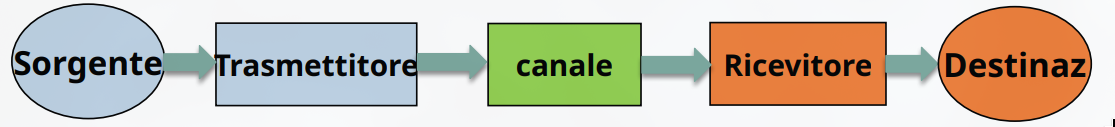
\includegraphics[width=0.8\textwidth]{images/01_01_SistemaTelecomunicazione.png}
    \caption{Sistema di Telecomunicazioni}
    \label{fig:01_01_SistemaTelecom}
\end{figure}

In particolare, come mostra la figura~\ref{fig:01_01_SistemaTelecom}, è composto dalle 
seguenti entità principali.
\begin{enumerate}
    \item \textbf{SORGENTE} : \textit{Genera informazione} sotto forma
        di una sequenza di simboli appartenenenti ad un \textit{alfabeto} $A$. 
        Spesso indicata con 'Tx'.
    \item \textbf{TRASMETTITORE}: \textit{Converte} la sequenza di
        simboli in una \textit{forma d'onda} (grandezza fisica, es tensione, onda
        elettromagnetica etc.) adatta ad essere trasmessa.
    \item \textbf{CANALE} : \textit{Mezzo fisico} (es cavo in ramo, fibra ottica, aria) 
        attraverso cui si propaga l'informazione.
    \item \textbf{RICEVITORE} : \textit{Elabora} l'informazione ricevuta.
        Spesso indicato con 'Rx'.
\end{enumerate}

% ----- RETI DI COMUNICAZIONE -----

\section{Reti di comunicazione}

I sistemi di telecomunicazioni sono \textit{interconnessi} a formare 
\textbf{reti di comunicazione}, come mostra la figura~\ref{fig:01_02_ReteTelecom}:

\newpage

\begin{figure}[!ht]
    \centering
    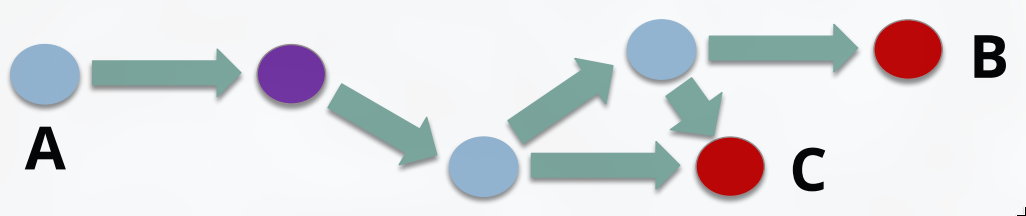
\includegraphics[width=0.8\textwidth]{images/01_02_RetiTelecom.png}
    \caption{Rete di Telecomunicazioni}
    \label{fig:01_02_ReteTelecom}
\end{figure}

\begin{remark}[RUOLI DINAMICI]
    I \textbf{ruoli non sono fissi}: ciascun nodo della rete può 
    essere sia trasmettitore che ricevitore.
\end{remark}

\subsection{Tipologie di comunicazione}

Possiamo classificare la comunicazione in base alle seguenti categorie:
\begin{itemize}
    \item \textbf{UNICAST} : Da \textit{punto a punto}.
    \item \textbf{MULTICAST} : Da un nodo ad \textit{altri punti}.
    \item \textbf{BROADCAST} : Da un nodo \textit{a tutti gli altri}.
\end{itemize}

\subsection{Direzione della comunicazione}

Un servizio può essere classificato come:
\begin{itemize}
    \item \textbf{UNIDIREZIONALE} (es. televisione)
    \item \textbf{BIDIREZIONALE}
        \begin{itemize}
            \item \textit{ASIMMETRICO} (es. web browsing)
            \item \textit{SIMMETRICO} (es. telefono)
        \end{itemize}
\end{itemize}

In particolare, i sistemi biderezionali sono a loro volta classificati anche in:
\begin{itemize}
    \item \textbf{HALF-DUPLEX} : la trasmissione può avvenire in entrambe le direzioni, ma
        \textit{non contemporaneamente}.
    \item \textbf{FULL-DUPLEX} : la trasmissione può avvenire nelle 
        due direzioni \textit{contemporaneamente}.
\end{itemize}

% ----- RUMORE E INTERFERENZE -----

\section{Rumore e Interferenze}

Ciascun entità del sistema di telecomunicazione è una possibile \textbf{fonte di rumore},
in particolare lo è il \textbf{canale}, a causa di \textit{rumore termico} e altre
\textit{distorsioni fisiche}.

\begin{definition}[RUMORE]
    Il rumore (o \textit{interferenza}) è una \textbf{fonte di errori}
    nella \textit{sequenza di simboli}.
\end{definition}

In altre parole, il rumore introduce \textbf{errori nei simboli trasmessi}.

Alla luce di ciò, si definiscono (per esempio):
\begin{itemize}
    \item \textbf{SNR} (\textit{Signal to Noise Ratio}) : Rapporto segnale/rumore, che quantifica
        la qualità dell'informazione ricevuta rispetto all'originale.
    \item \textbf{BER} (\textit{Bit Error Rate}) : Nelle trasmissioni \textit{digitali} quantifica
        la probabilità di \textit{errore su un bit} ($P_{\text{bit}}\coloneqq P[\hat{b}_k \ne b_k]$).
\end{itemize}

% ------------------------------------------------------------------------------------
%                               SEGNALI
% ------------------------------------------------------------------------------------

\chapter{Segnali}

Nelle reti di telecomunicazione, le informazioni sono \textit{trasmesse attraverso segnali}, 
ovvero dei \textit{modelli matematici di grandezze fisiche}.

\begin{definition}[SEGNALE]
    Un segnale è una \textbf{funzione} che associa un \textbf{valore} ad
    ogni \textbf{istante di tempo}:
    \[
        s(t) : \mathbb{R} \to \mathbb{C}
    \] 
\end{definition}

% ----- NOTA SULLA RAPPRESENTAZIONE -----

\section{Note sulla rappresentazione complessa}

In generale, si utilizza una \textbf{funzione complessa di variabile reale} per 
una questione di "comodità" matematica.
Il perchè appararirà più chiaro in futuro. Per ora ricordiamo l'uso 
della seguente notazione (usiamo $j$ per l'unità immaginaria):

\begin{itemize}
    \item Parte reale: $\text{Re}[s(t)]=s_R(t)$
    \item Parte immaginaria: $\text{Im}[s(t)] = s_I(t)$
    \item Complesso coniugato: $s^*(t)=\bar{s}(t) = s_R(t) - js_I(t)$
    \item Modulo: $|s(t)| = \sqrt{s_R^2(t) + s_I^2(t)} = \sqrt{s(t)s^*(t)}$
    \item Fase: $\text{arg}[s(t)] = \angle s(t) = \arctan(\frac{s_I(t)}{s_R(t)})$
\end{itemize}

% ----- TIPOLOGIE SEGNALI -----

\section{Tipologie di segnali}

Possiamo distinguere i segnali in base a:
\begin{itemize}
    \item \textbf{VALORI}
        \begin{itemize}
            \item \textbf{DISCRETI}: $s_R(t),s_I(t)\in \mathbb{Z}$
            \item \textbf{CONTINUI} : $s_R(t),s_I(t)\in \mathbb{R}$
        \end{itemize}
    \item \textbf{TEMPO}
        \begin{itemize}
            \item \textbf{DISCRETO}: $t\in \mathbb{Z}$
            \item \textbf{CONTINUO} : $t\in \mathbb{R}$
        \end{itemize}
\end{itemize}

Tale suddivisione è riassunta nella tabella~\ref{tb:01_01_tipologie_segnali}.

\begin{table}[!ht]
    \centering
    \renewcommand{\arraystretch}{1.6} 
    \begin{tabular}{|l|c|c|}
        \hline
        & Tempo discreto & Tempo continuo \\
        \hline
        
        Valori discreti & \cellcolor{orange!40}DIGITALI & no nome \\
        \hline
        
        Valori continui & no nome & \cellcolor{orange!40}ANALOGICI \\
        \hline
    \end{tabular}
    \caption{Tipologie di Segnali}
    \label{tb:01_01_tipologie_segnali}
\end{table}

La figura~\ref{fig:02_01_esempi_segnali} mostra un esempio di segnale analogico e di uno digitale.

\begin{figure}[!ht]
    \centering
    % --- Primo Plot: Segnale Analogico ---
    \begin{minipage}{0.48\textwidth}
        \centering
        \begin{tikzpicture}
            \begin{axis}[
                width=\textwidth,
                height=5cm,
                axis lines=middle,
                xlabel={$t$},
                ylabel={$s(t)$},
                xmin=0, xmax=2.2,
                ymin=-1.5, ymax=1.5,
                xtick={0, 0.5, 1, 1.5, 2},
                ytick={-1, 0, 1},
                grid=major,
                grid style={dashed, gray!30},
                title={Segnale Analogico},
                title style={font=\bfseries\small},
                xlabel style={below right},
                ylabel style={above left},
            ]
                \addplot[thick, nord10, domain=0:2, samples=200] {sin(deg(2*pi*x))};
            \end{axis}
        \end{tikzpicture}
    \end{minipage}\hfill
    % --- Secondo Plot: Segnale Digitale ---
    \begin{minipage}{0.48\textwidth}
        \centering
        \begin{tikzpicture}
            \begin{axis}[
                width=\textwidth,
                height=5cm,
                axis lines=middle,
                xlabel={$n$},
                ylabel={$s[n]$},
                xmin=-0.5, xmax=7.5,
                ymin=-0.5, ymax=1.5,
                xtick={0,1,2,3,4,5,6,7},
                ytick={0,1},
                grid=major,
                grid style={dashed, gray!30},
                title={Segnale Digitale},
                title style={font=\bfseries\small},
                xlabel style={below right},
                ylabel style={above left},
            ]
                \addplot[
                    ycomb, 
                    thick, 
                    nord11, 
                    mark=*, 
                    mark options={fill=nord11, scale=1.2}
                ] coordinates {
                    (0,1) (1,0) (2,1) (3,0) (4,0) (5,1) (6,1) (7,0)
                };
            \end{axis}
        \end{tikzpicture}
    \end{minipage}
    \caption{Un segnale analogico e un segnale digitale.}
    \label{fig:02_01_esempi_segnali}
\end{figure}

In particolare, per i segnali a \textbf{tempo discreto} definiamo il:

\begin{definition}[PERIODO DI SEGNALE]
    Il periodo di segnale $T_s$ è il periodo con il quale il segnale viene campionato.
    In tal senso risulta comodo usare la notazione seguente:
    \[
            t = nT_s, n\in \mathbb{Z} \implies s[n]\coloneqq s(nT_s)\in \mathbb{C}
    \] 
\end{definition}

% ----- ESEMPI SEGNALI -----

\section{Esempi di segnali}
\subsection{Impulso Rettangolare}

L'impulso rettangolare è così definito:

\begin{definition}[IMPULSO RETTANGOLARE]
    \[
        \text{rect}(t) \coloneqq \begin{cases}
            1 & |t| \le \frac{1}{2} \\
            0 & \text{altrimenti}
        \end{cases} 
    \] 
\end{definition}

\begin{figure}[!ht]
    \centering
    \begin{tikzpicture}[scale = 0.8]
        \begin{axis}[
            width=0.8\textwidth,
            height=5cm,
            axis lines=middle,
            xlabel={\(t\)},
            ylabel={\(s(t)\)},
            xmin=-1.1, xmax=1.1,
            ymin=-0.2, ymax=1.5,           
            xtick={-1, -0.5, 0, 0.5, 1},
            ytick={0, 1},
            grid=major,
            grid style={dashed, nord3!30},       
            axis line style={nord0},             
            tick style={nord0},                  
            tick label style={color=nord0},      
            xlabel style={below right, color=nord0},
            ylabel style={above left, color=nord0}
        ]
        \addplot[thick, nord10] coordinates {
            (-0.5, 0) (-0.5, 1) (0.5, 1) (0.5, 0)
        };
        \end{axis}
    \end{tikzpicture}
    \caption{Impulso rettangolare.}
\end{figure}

\subsection{Triangolo}

La funzione triangolo è definita come segue:

\begin{definition}[TRIANGOLO]
    \[
        \text{triang}(t) \coloneqq \begin{cases}
            1-|t| & |t| \le 1 \\
            0 & \text{altrimenti}
        \end{cases} 
    \] 
\end{definition}

\begin{figure}[!ht]
    \centering
    \begin{tikzpicture}[scale = 0.8]
        \begin{axis}[
            width=0.75\textwidth,
            height=5cm,
            axis lines=middle,
            xlabel={$t$},
            ylabel={$s(t)$},
            xmin=-2.5, xmax=2.5,
            ymin=-0.5, ymax=1.5,
            xtick={-2,-1,0,1,2},
            ytick={0,1},
            grid=major,
            grid style={dashed, gray!30},
            xlabel style={below right},
            ylabel style={above left},
        ]
            \addplot[thick, nord10] coordinates {
                (-2.5,0) (-1,0) (0,1) (1,0) (2.5,0)
            };
            
        \end{axis}
    \end{tikzpicture}
    \caption{Segnale triangolo.}
    \label{fig:02_03segnale_tri}
\end{figure}

\subsection{Esponenziale complesso}

Un esponenziale complesso è un segnale del tipo:

\begin{definition}[ESPONENZIALE COMPLESSO]
    \[
        s(t) = e^{j 2\pi f_{0}t} = \cos (2\pi f_{0}t) + j \sin (2\pi f_{0}t)
    \] 
\end{definition}

Notiamo che:

\begin{remark}
    E' un segnale \textbf{periodico}:
    \begin{itemize}
        \item Di \textit{frequenza} $f_{0}$
        \item Di periodo $T_{0} = \frac{1}{f_{0}}$
        \item Di pulsazione $\omega_{0} = 2\pi f_{0}$
        \item Di modulo $|e^{j 2\pi f_{0}t}|=1$
        \item Di fase $2\pi f_{0}t$
    \end{itemize}
\end{remark}

Un esempio di questo segnale è mostrato nella figura~\ref{fig:02_04:esponenziale_complesso}

\begin{figure}[!ht]
    \centering
    \begin{tikzpicture}[scale = 0.8]
        \begin{axis}[
            width=0.8\textwidth,
            height=0.65\textwidth,
            view={60}{30}, 
            axis lines=middle,
            xlabel={$t$},
            ylabel={$\mathrm{Re}$},
            zlabel={$\mathrm{Im}$},
            xmin=0, xmax=4*pi,
            ymin=-1.5, ymax=1.5,
            zmin=-1.5, zmax=1.5,
            xtick={0, pi, 2*pi, 3*pi, 4*pi},
            xticklabels={$0$, $\pi$, $2\pi$, $3\pi$, $4\pi$},
            ytick={-1,0,1},
            ztick={-1,0,1},
            grid=major,
            grid style={dashed, gray!30},
            xlabel style={below right},
            ylabel style={above left},
            zlabel style={above left},
        ]
            % Spirale principale (elica)
            \addplot3[
                domain=0:4*pi,
                samples=200,
                samples y=0, 
                variable=\t,
                thick,
                nord10,
            ] ({\t}, {cos(deg(\t))}, {sin(deg(\t))});
            
            % Proiezione sul piano t-Re 
            \addplot3[
                domain=0:4*pi,
                samples=200,
                samples y=0,
                variable=\t,
                dashed,
                nord14,
                opacity=0.5,
            ] ({\t}, {cos(deg(\t))}, {-1.5});
            
            % Proiezione sul piano t-Im 
            \addplot3[
                domain=0:4*pi,
                samples=200,
                samples y=0,
                variable=\t,
                dashed,
                nord11,
                opacity=0.5,
            ] ({\t}, {1.5}, {sin(deg(\t))});
            
            % Cerchio di proiezione sul piano Re-Im a t=0 
            \addplot3[
                domain=0:360,
                samples=100,
                samples y=0,
                variable=\a,
                dashed,
                nord3,
                opacity=0.4,
            ] ({0}, {cos(\a)}, {sin(\a)});
        \end{axis}
    \end{tikzpicture}
    \caption{Segnale esponenziale complesso}
    \label{fig:02_04:esponenziale_complesso}
\end{figure}

\subsection{Funzione sinc}

Un altro segnale molto importante è il seguente:

\begin{definition}[SINC]
    \[
        \text{sinc}(t) = \frac{\sin (\pi t)}{\pi t}
    \] 
\end{definition}

\begin{figure}[!ht]
    \centering
    \begin{tikzpicture}[scale = 0.8]
        \begin{axis}[
            width=0.85\textwidth,
            height=6cm,
            axis lines=middle,
            xlabel={$t$},
            ylabel={$\mathrm{sinc}(t)$},
            xmin=-5, xmax=5,
            ymin=-0.4, ymax=1.2,
            xtick={-5,-4,-3,-2,-1,0,1,2,3,4,5},
            ytick={-0.2,0,0.2,0.4,0.6,0.8,1},
            grid=major,
            grid style={dashed, gray!30},
            xlabel style={below right},
            ylabel style={above left},
            declare function={
                sinc(\x) = \x == 0 ? 1 : sin(deg(pi*\x))/(pi*\x);
            },
        ]
            % Plot della funzione sinc
            \addplot[
                thick,
                nord10,
                domain=-5:5,
                samples=400,
                smooth,
            ] {sinc(x)};
            
            % Evidenzia il punto in t=0 con un marker
            \addplot[
                only marks,
                mark=*,
                mark size=1.8pt,
                nord11,
            ] coordinates {(0,1)};
            
        \end{axis}
    \end{tikzpicture}
    \caption{Segnale sinc}
    \label{fig:02_05_segnale_sinc}
\end{figure}

Spesso ci si riferisce a questa funzione come "\textbf{sinc normalizzata}".

E' inoltre interessante notare che:

\begin{remark}
    Note sulla funzione sinc normalizzata:
    \begin{enumerate}
        \item $\lim_{t\to 0} \text{sinc}(t) = 1$
        \item La funzione si \textbf{annulla} per tutti gli 
            \textbf{interi non nulli}: $\text{sinc}(t)=0\forall k\in \mathbb{Z}\setminus \{0\}$
    \end{enumerate}
\end{remark}

% ----- OPERAZIONI SU SEGNALI -----

\section{Operazioni sui segnali}

\subsection{Ritardo/anticipo di un segnale}

Dato un segnale $s(t)$, possiamo \textit{traslarlo nel tempo} come segue:

\begin{definition}[TRASLAZIONE SEGNALE]
    \[
        \tilde{s}(t) \coloneqq s(t-t_{0})
    \] 
\end{definition}

In particolare, abbiamo:
\begin{itemize}
    \item \textbf{RITARDO} se $t_{0}>0$.
    \item \textbf{ANTICIPO} se $t_{0}<0$.
\end{itemize}

\begin{figure}[!ht]
    \centering
    \begin{tikzpicture}
        \begin{axis}[
            width=0.8\textwidth,
            height=5cm,
            axis lines=middle,
            xlabel={\(t\)},
            ylabel={\(s(t)\)},
            xmin=-1.5, xmax=3.5,
            ymin=-0.2, ymax=1.8, % Spazio sufficiente per le etichette
            xtick={-0.5, 0, 0.5, 1, 1.5, 2, 2.5},
            ytick={0, 1},
            grid=major,
            grid style={dashed, nord3!30},
            axis line style={nord0},
            tick style={nord0},
            tick label style={color=nord0},
            xlabel style={below right, color=nord0},
            ylabel style={above left, color=nord0}
        ]
        
        \addplot[thick, dashed, nord10] coordinates {
            (-0.5, 0) (-0.5, 1) (0.5, 1) (0.5, 0)
        };
        \node[nord10, anchor=south] at (axis cs: -0.5, 1.05) {\(s(t)\)};

        \addplot[thick, nord11] coordinates {
            (1.5, 0) (1.5, 1) (2.5, 1) (2.5, 0)
        };
        \node[nord11, anchor=south] at (axis cs: 2, 1.05) {\(\tilde{s}(t) = s(t-2)\)};

        \draw[<->, >=stealth, thick, nord3] (axis cs: 0, 0.6) -- (axis cs: 2, 0.6);
        \node[nord3, anchor=south] at (axis cs: 1, 0.6) {\(t_0 = 2\)};

        \end{axis}
    \end{tikzpicture}
    \caption{Traslazione del rettangolo.}
\end{figure}

\subsection{Scalamento di un segnale}

Nella trasmissione di un segnale, il ricevente ha spesso bisogno di un
\textbf{amplificatore} che \textit{scali il segnale}. Questo perchè
il segnale ricevuto risulta smorzato/attenuate durante la trasmissione.

\begin{definition}[SCALAMENTO SEGNALE]
    \[
        \tilde{s}(t) \coloneqq As(t)
    \] 
\end{definition}

Per un amplificatore, chiaramente vale $A>1$.

\begin{figure}[!ht]
    \centering
    \begin{tikzpicture}
        \begin{axis}[
            width=0.8\textwidth,
            height=5cm,
            axis lines=middle,
            xlabel={\(t\)},
            ylabel={\(s(t), \tilde{s}(t)\)},
            xmin=-1.1, xmax=1.1,
            ymin=-0.2, ymax=2.5, % Spazio per l'ampiezza 2
            xtick={-1, -0.5, 0, 0.5, 1},
            ytick={0, 1, 2},
            grid=major,
            % Applicazione della palette Nord
            grid style={dashed, nord3!30},
            axis line style={nord0},
            tick style={nord0},
            tick label style={color=nord0},
            xlabel style={below right, color=nord0},
            ylabel style={above left, color=nord0}
            ]

            % Segnale originale s(t) in blu tratteggiato
            \addplot[thick, dashed, nord10] coordinates {
                    (-0.5, 0) (-0.5, 1) (0.5, 1) (0.5, 0)
                };
            \node[nord10, anchor=south] at (axis cs: -0.2, 1.05) {\(s(t)\)};

            % Segnale scalato \tilde{s}(t) = 2s(t) in rosso continuo
            \addplot[thick, nord11] coordinates {
                    (-0.5, 0) (-0.5, 2) (0.5, 2) (0.5, 0)
                };
            \node[nord11, anchor=south] at (axis cs: 0.3, 2.05) {\(\tilde{s}(t) = 2s(t)\)};
        \end{axis}
    \end{tikzpicture}
    \caption{Scalamento dell'ampiezza di un segnale.}
\end{figure}

\begin{remark}
    In generale, $A$ può assumere qualsiasi valore reale,
    \textit{anche negativo} (in tal caso il segnale è riflesso
    rispetto all'asse delle ascisse)
\end{remark}

\subsection{Scalamento nel tempo}

Dato un segnale, oltre che scalarne l'ampiezza, possiamo scalarlo
anche nel tempo:

\begin{definition}[SCALEMENTO NEL TMEPO]
    \[
        \tilde{s}(t) \coloneqq s\left( \frac{t}{B} \right)
    \] 
\end{definition}

\begin{figure}[!ht]
    \centering
    \begin{tikzpicture}
        \begin{axis}[
            width=0.8\textwidth,
            height=5cm,
            axis lines=middle,
            xlabel={\(t\)},
            ylabel={\(s(t), \tilde{s}(t)\)},
            xmin=-1.8, xmax=1.8,
            ymin=-0.2, ymax=1.8, % Spazio per le etichette
            xtick={-1, -0.5, 0, 0.5, 1},
            ytick={0, 1},
            grid=major,
            % Applicazione della palette Nord
            grid style={dashed, nord3!30},
            axis line style={nord0},
            tick style={nord0},
            tick label style={color=nord0},
            xlabel style={below right, color=nord0},
            ylabel style={above left, color=nord0}
        ]
        
        % Segnale originale s(t) in blu tratteggiato
        \addplot[thick, dashed, nord10] coordinates {
            (-0.5, 0) (-0.5, 1) (0.5, 1) (0.5, 0)
        };
        \node[nord10, anchor=south] at (axis cs: 0.65, 0.25) {\(s(t)\)};

        % Caso |B| > 1 (Allungato): \tilde{s}(t) = s(t/2) in rosso
        \addplot[thick, nord11] coordinates {
            (-1, 0) (-1, 1) (1, 1) (1, 0)
        };
        \node[nord11, anchor=south] at (axis cs: -1.4, 0.25) {\(\tilde{s}(t) = s(\frac{t}{2})\)};

        % Caso |B| < 1 (Contratto): \tilde{s}(t) = s(2t) in verde
        \addplot[thick, nord14] coordinates {
            (-0.25, 0) (-0.25, 1) (0.25, 1) (0.25, 0)
        };
        \node[nord14, anchor=south] at (axis cs: -0.4, 1.05) {\(\tilde{s}(t) = s(2t)\)};

        \end{axis}
    \end{tikzpicture}
    \caption{Scalamento nel tempo di un segnale.}
\end{figure}

Ragionando su $B$ notiamo che:

\begin{remark}
    Distinguiamo 3 casi:
    \begin{itemize}
        \item Se $B<0$, il segnale è \textit{riflesso rispetto alle ordinate}.
        \item Se $|B|>1$ il segnale è \textbf{allungato}.
        \item Se $|B|<1$ il segnale è \textbf{contratto}.
    \end{itemize}
\end{remark}

\subsection{Combinazione di operazioni}

In generale, possiamo combinare tutte le operazioni viste sopra
per ottenere un nuovo segnale:

\begin{definition}[COMBINAZIONE DI OPERAZIONI]
    \[
        \tilde{s}(t) = As \left( \frac{t-t_{0}}{B} \right)
    \] 
\end{definition}

Come procediamo in tali casi? Procediamo come mostrato sotto:
\[
    s(t) \mapsto s_{1}(t) = s(t-t_{0}) \mapsto s_{2}(t) = s\left( \frac{t-t_{0}}{B} \right) 
    \mapsto s_{3} = As\left( \frac{t-t_{0}}{B} \right) = \tilde{s}(t)
\]

% ----- GRANDEZZE ASSOCIATE -----

\section{Grandezze associate ad un segnale}

\subsection{Valor medio}

Per un segnale a \textit{tempo continuo} $s(t)$, il suo \textit{valor medio} nell'intervallo
$[t_{1},t_{2}]$ è definito come segue:

\begin{definition}[VALOR MEDIO - TC]
    \[
        m_s(t_{1},t_{2}) = \frac{1}{t_{2}-t_{1}} \int_{t_{1}}^{t_{2}} s(t)dt
    \] 
\end{definition}

Se invece il segnale è a \textit{tempo discreto} abbiamo, in
un intervallo $[n_{1},n_{2}]$:

\begin{definition}[VALOR MEDIO - TD]
    \[
        m_s(n_{1},n_{2}) = \frac{1}{n_{2}-n_{1}} \sum_{n=n_{1}}^{n_{2}} s(nT)
    \] 
\end{definition}

Possiamo estendere il concetto di valor medio a tutto l'asse reale:

\begin{prop}[VALOR MEDIO SU TUTTO L'ASSE]
    Valor medio su tutto l'asse a tempo continuo:
    \[
        m_s = \lim_{u\to\infty} \frac{1}{2u} \int_{-u}^{u} s(t)dt
    \]
    Valor medio su tutto l'asse a tempo discreto:
    \[
        m_s = \lim_{k\to\infty} \frac{1}{2k} \sum_{n=-k}^{k} s(nT)
    \] 
\end{prop}

E' facile intuire che:

\begin{remark}[VALOR MEDIO DI SEGNALI DI DURATA FINITA]
    Se un segnale ha \textbf{durata finita} (es. $\text{rect}$), l'area
    totale è finita e, di conseguenza, il \textbf{valor medio è nullo}.
\end{remark}

\subsection{Energia}

Possiamo definire l'\textbf{energia} associata ad un segnale come segue.
Per un segnale a tempo continuo:

\begin{definition}[ENERGIA DI UN SEGNALE - TC]
    \[
        E_s = \int_{-\infty}^{+\infty} s(t)^2 dt
    \] 
\end{definition}

Per un segnale a tempo discreto:

\begin{definition}[ENERGIA DI UN SEGNALE - TD]
    \[
        E_s = T\sum_{n=-\infty}^{+\infty} s(nT)^2
    \] 
\end{definition}

E' utile osservare che l'energia di un segnale è \textbf{invariante} rispetto
a \textbf{traslazioni temporali}.

Inoltre, essendo l'energia del segnale una quantità quadratica, bisogna
fare attenzione all'energia trasportata dalla \textbf{somma di due segnali}.
Consideriamo per esempio due segnali a tempo continuo $s_{1}(t)$ e $s_{2}(t)$ 
(il caso discreto è analogo) e la loro somma $s(t)=s_{1}(t)+s_{2}(t)$:
Cominciamo calcolando il modulo al quadrato del segnale:
\[
    \begin{aligned}
        |s_{1} + s_{2}|^2 &= (s_{1}+s_{2})(s_{1}^* + s_{2}^*) \\ 
                   &= |s_{1}|^2 + |s_{2}|^2 + s_{1}s_{2}^* + s_{2}s_{1}^* 
                   =  |s_{1}|^2 + |s_{2}|^2 + (s_{1}s_{2}^*) + (s_{1}s_{2}^*)^* \\ 
                   &= |s_{1}|^2 + |s_{2}|^2 + 2 \text{Re}(s_{1}s_{2}^*)
    \end{aligned}
\]
Sostituendo nella definizione otteniamo allora:

\begin{warning}[ENERGIA DELLA SOMMA DI DUE SEGNALI]
    \[
    \begin{aligned}
        E_s &= \int_{-\infty}^{\infty} \left[ |s_{1}|^2 + |s_{2}|^2 + 2 \text{Re}(s_{1}s_{2}^*) \right] dt \\ 
            &= E_{s_{1}} + E_{s_{2}} + 2 \text{Re} 
            \left( \int_{-\infty}^{+\infty} s_{1}(t)s_{2}^*(t) dt\right)
    \end{aligned}
    \] 
\end{warning}

Possiamo quindi notare che:

\begin{remark}
    Se i due segnali hanno \textbf{supporto temporale disgiunto}, allora l'energia
    risultante è semplicemente la somma delle due energie:
    \[
        D_{s_{1}} \cap D_{s_{2}} = \emptyset \implies s_{1}s_{2}^* = 0 \forall t 
        \implies E_s = E_{s_{1}} + E_{s_{2}}
    \] 
\end{remark}

\subsection{Potenza media}

Possiamo definire anche la potenza media di un segnale in certo intervallo.
Per un segnale a tempo continuo $s(t)$ nell'intervallo $[t_{1},t_{2}]$:

\begin{definition}[POTENZA MEDIA - TC]
    \[
        P_s = \frac{1}{t_{2}-t_{1}} \int_{t_{1}}^{t_{2}} s^2(t)dt
    \] 
\end{definition}

Per un segnale a tempo discreto $s(nT)$ nell'intervallo $[n_{1},n_{2}]$:

\begin{definition}[POTENZA MEDIA - TD]
    \[
        P_s = \frac{1}{n_{1}-n_{2}} \sum_{n=n_{1}}^{n_{2}} s^2(nT)
    \] 
\end{definition}

Chiaramente, come prima abbiamo fatto con il valor medio, possiamo estendere il concetto
di potenza media su tutto l'asse $(-\infty,+\infty)$ semplicemente applicando il limite.


% ------------------------------------------------------------------------------------
%                               SISTEMI e TRASFORMAZIONI SUI SEGNALI
% ------------------------------------------------------------------------------------

\chapter{Sistemi e trasformazioni sui segnali}

Ora che abbiamo discusso cosa sono i segnali, possiamo passare alla loro elaborazione.
Per farlo, abbiamo bisogno di un \textbf{sistema}, che è banalmente:

\begin{definition}[SISTEMA]
    Un sistema è un \textbf{insieme di componenti fisici} che 
    \textbf{applica una trasformazione} ad un \textbf{segnale di ingresso} $x(t)$
    per produrre un \textbf{segnale d'uscita} $y(t)$.
\end{definition}

\begin{figure}[!ht]
    \centering
    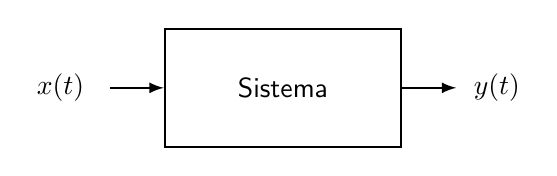
\begin{tikzpicture}[>=latex]
        \node[draw, thick, minimum width=3cm, minimum height=1.5cm] (lti) at (0,0) {\textsf{Sistema}};
        \draw[->, thick] (-2.2, 0) -- (lti.west);
        \node[anchor=east] at (-2.4, 0) {$x(t)$};
        \draw[->, thick] (lti.east) -- (2.2, 0);
        \node[anchor=west] at (2.3, 0) {$y(t)$};
    \end{tikzpicture}
    \caption{Schematizzazione di un sistema}
\end{figure}

Sostanzialmente, i sistemi sono delle \textit{"realizzazioni fisiche"} di funzioni 
che mappano segnali in altri segnali, permettondoci di \textbf{manipolarli}: combinando
componenti diverse e secondo determinati schemi possiamo \textbf{realizzare trasformazioni
"a piacimento"}.

Alcuni esempi di sistemi sono:
\begin{itemize}
    \item \textbf{FILTRI} (passa-basso, passa-alto, passa-banda)
    \item \textbf{AMPLIFICATORI}
    \item \textbf{LINEE DI TRASMISSIONE}
    \item \textbf{MICROPROCESSORI} (essenzialmente sistemi molto complessi)
\end{itemize}

Vediamo di seguito un esempio di (semplice) sistema comunemente usato: 
\begin{exa}[MEDIA MOBILE - MOVING AVERAGE]
    \[
        T: y(nT) = \frac{x(nT) + x(nT-T) + x(nT-2T)}{3}
    \] 
\end{exa}

L'output di tale sistema è la media degli ultimi tre valori del segnale discreto
in ingresso.

% ----- SISTEMI FONDAMENTALI -----

\section{Sistemi fondamentali}
\subsection{Sistemi lineari}

Particolarmente importanti sono i sistemi lineari:

\begin{definition}[SISTEMA LINEARE]
    Diciamo che un sistema $T$ è \textbf{lineare} se vale
    il \textbf{principio di sovrapposizione degli effetti}:
    \[
        T[\alpha x_{1}(t) + \beta x_{2}(t)] = \alpha T[x_{1}(t)] + \beta T[x_{2}(t)]
    \] 
\end{definition}

In altre parole, un sistema lineare rappresenta una \textbf{trasformazione lineare del segnale}
di ingresso. Attenzione al seguente esempio:

\begin{exa}[ESEMPIO FUORVIANTE]
    Il sistema caratterizzato da
    \[
        T: x(t) \mapsto y(t) = x(t-1) + 2
    \] 
    è lineare? La risposta è \textbf{no}!
\end{exa}

Infatti, considerando per esempio due segnali di ingresso $x_{1}(t)$ e $x_{2}(t)$,
abbiamo:
\[
    \begin{aligned}
        T[x_{1}(t)] &= x_{1}(t-1) + 2 \\
        T[x_{2}(t)] &= x_{2}(t-1) + 2 \\
        T[x_{1}(t) + x_{2}(t)] &= x_{1}(t-1) + x_{2}(t-1) + 2 \\ 
                               &\ne T[x_{1}(t)] + T[x_{2}(t)]
    \end{aligned}
\]
Del resto, la trasformazione applicata dal sistema è \textit{affine}, \textbf{non} \textit{lineare}.

In generale, affermiamo che:

\begin{prop}[SISTEMI LINEARI]
    I sistemi lineari sono \textbf{tutti e soli} i sistemi in
    cui il \textit{segnale di ingresso} compare nell'\textit{uscita}
    \textbf{solo} con \textbf{potenza pari a uno}.
\end{prop}

Spesso, sistemi di questo tipo possono essere scritti nella forma:
\[
    T: x(t) \mapsto y(t) = Ax(t)
\]
Dove $A$ è una matrice.
E' importante notare che le entrate di questa matrice
\textbf{non sono necessariamente costanti}.

\begin{exa}
    Il seguenee sistema è \textbf{lineare}:
    \[
        y(t) = x(t)\cos (2\pi f_{0}t)
    \] 
    Anche il seguente sistema, sebbene non sia rappresentabile in 
    forma matriciale, è \textbf{lineare}:
    \[
        y(t) = \int_{t-1}^{t} x(\tau )d \tau
    \]
\end{exa}

\subsection{Sistemi tempo invarianti}

Un'altra importante categoria di sistemi è quella dei \textbf{sistemi tempo invarianti}.

\begin{definition}[SISTEMI TEMPO INVARIANTI]
    Un sistema $T$ è detto \textbf{tempo invariante} se soddisfa:
    \[
        T[x(t)] = y(t) \implies T[x(t-t_{0})] = y(t-t_{0})
    \] 
\end{definition}

Osserviamo che il sistema \textbf{media mobile} introdotto sopra è
\textbf{tempo invariante}. Infatti, se consideriamo $x_{1}(nT)=x(nT)$ e $x_{2}(t)=x((n-n_{0})T)$ abbiamo:
\[
    \begin{aligned}
        y_{1}(nT) &= \frac{1}{3}\left[ x(nT) + x(nT-T) + x(nT-2T) \right] \\ 
        y_{2}(nT) &= \frac{1}{3}\left[ x((n-n_{0})T) + x((n-n_{0})T - T) + x((n-n_{0})T - 2T) \right] \\ 
                 &= y_{1}((n-n_{0})T)
    \end{aligned}
\]
Al contrari osserviamo, sempre su uno degli esempi visti prima:

\begin{remark}
    Il sistema $y(t)=x(t)\cos (2\pi f_{0}t)$ era \textit{lineare}, ma
    \textbf{non è tempo invariante}.
\end{remark}

Verifichiamolo per completezza, considerando $x_{1}(t) = x(t)$ e $x_{2}(t) = x(t-t_{0})$:
\[
    \begin{aligned}
        y_{1}(t) &= x(t)\cos (2\pi f_{0}t) \\ 
        y_{2}(t) &= x(t-t_{0})\cos (2\pi f_{0}t) \\ 
                 &\ne y_{1}(t-t_{0})
    \end{aligned}
\]
\begin{remark}
    Il sistema \textbf{non è tempo-invariante} perchè il \textbf{coefficiente}
    ha una \textbf{dipendenza dal tempo} $t$: lo \textit{stesso segnale}
    viene \textit{trasformato diversamente} in base all'\textit{istante
    in cui entra nel sistema}.
\end{remark}

% ----- SISTEMI CONVOLUZIONALI -----

\section{Sistemi convoluzionali}

A questo punto possiamo definire i sistemi convoluzionali:

\begin{definition}[SISTEMI LTI e CONVOLUZIONALI]
    Se un sistema è \textbf{sia lineare}, \textbf{sia tempo invariante}, è
    definito \textbf{lineare, tempo invariante}, abbreviato \textbf{LTI}.

    I \textbf{sistemi convoluzionali} (per noi) sono i \textbf{sistemi LTI}.
\end{definition}

E' opportuno notare che, in realtà, esistono \textit{"casi patologici"} di 
sistemi LTI che \textit{non sono convoluzionali}, ma noi non ce ne occuperemo.

In ogni caso, tali sistemi sono detti convoluzionali per il seguente motivo:

\begin{prop}[SISTEMI CONVOLUZIONALI]
    Dato un sistema convoluzionale, la sua \textbf{risposta} $y(t)$
    ad un \textbf{ingresso} $x(t)$ è esprimibile come segue:
    \[
        y(t) = x(t) \ast h(t)
    \] 
    Cioè la risposta è data dall \textbf{convoluzione} tra l'\textbf{ingresso}
    $x(t)$ e la \textbf{risposta impulsiva} $h(t)$, che è \textit{caratteristica} 
    del sistema.
\end{prop}

\begin{figure}[!ht]
    \centering
    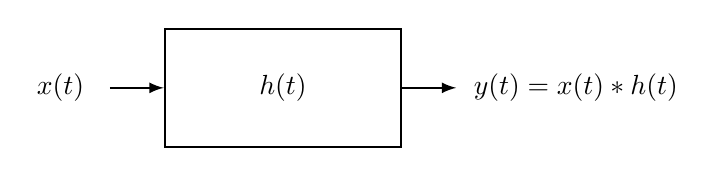
\begin{tikzpicture}[>=latex]
        \node[draw, thick, minimum width=3cm, minimum height=1.5cm] (lti) at (0,0) {$h(t)$};
        \draw[->, thick] (-2.2, 0) -- (lti.west);
        \node[anchor=east] at (-2.4, 0) {$x(t)$};
        \draw[->, thick] (lti.east) -- (2.2, 0);
        \node[anchor=west] at (2.3, 0) {$y(t) = x(t)\ast h(t)$};
    \end{tikzpicture}
    \caption{Schematizzazione di un sistema convoluzionale}
\end{figure}

\subsection{Convoluzione}

Per capire meglio di cosa stiamo parlando, definiamo l'operazione
di convoluzione:

\begin{definition}[CONVOLUZIONE]
    Date due funzioni $x(t)$ e $y(t)$, la loro \textbf{convoluzione} è
    definita come segue:
    \[
        z(t) = x(t) \ast y(t) = \int_{-\infty}^{+\infty} x(\tau )y(t-\tau )d\tau
    \] 
\end{definition}

\subsection{Proprietà della convoluzione}

Elenchiamo di seguito alcune proprietà utili delle convoluzioni:
\begin{enumerate}
    \item \textbf{COMMUTATIVITA'}: $f\ast g = g\ast f$.
    \item \textbf{ASSOCIATIVITA'}: $f\ast (g \ast h) = .(f\ast g)\ast h$
    \item \textbf{DISTRIBUTIVITA'} (rispetto alla somma): $f\ast (g+h) = (f\ast g) + (f\ast h)$.
\end{enumerate}

Sono utili anche i seguenti fatti:
\begin{enumerate}
    \item L'area del segnale $z(t)$ è uguale al \textbf{prodotto delle aree}.
    \item La durata del segnale $z(t)$ è uguale alla \textbf{somma delle durate}.
\end{enumerate}

\subsection{Impulso di Dirac}

L'elemento neutro per la convoluzione è l'impulso di Dirac:

\begin{definition}[IMPULSO DI DIRAC]
    \[
        \delta(t) \coloneqq \begin{cases}
            0 & \forall t\ne 0 \\ 
            +\infty & t = 0
        \end{cases}
    \]
\end{definition}

\begin{figure}
    \centering
    \begin{tikzpicture}[scale = 0.8]
        \begin{axis}[
            width=10cm,
            height=8cm,
            xmin=-2.1, xmax=2.1,
            ymin=-0.25, ymax=1.25,
            xtick={-2,-1,0,1,2},
            minor x tick num=4, 
            ytick={-0.2, 0.0, 0.2, 0.4, 0.6, 0.8, 1.0, 1.2},
            yticklabel style={
                /pgf/number format/fixed,
                /pgf/number format/precision=1
            },
            minor y tick num=1,
            xlabel={x},
            tick align=inside,
            axis on top,
            thick,
            tick style={thick, black}
            ]
            \draw[nord11, thick] (axis cs:-2.1,0) -- (axis cs:2.1,0);
            \draw[nord11, thick, ->, >=stealth, shorten <= 3pt] (axis cs:0,0) -- (axis cs:0,1);
            \addplot[nord11, thick, mark=*, 
                mark options={fill=white, scale=1.2}, only marks] coordinates {(0,0)};

        \end{axis}
    \end{tikzpicture}
    \caption{Impulso di Dirac}
\end{figure}

E' importante notare che vale:
\[
    \text{Area}[\delta(t)] = \int_{-\infty}^{+\infty}\delta(t) dt = 1    
\] 

\begin{prop}[ELEMENTO NEUTRO PER LA CONVOLUZIONE]
    L'impulso di Dirac è l'elemento neutro per la convoluzione.
    Dato un segnale $x(t)$, abbiamo:
    \[
        \begin{aligned}
            x(t) \ast \delta(t) &= x(t) \\ 
            x(t) \ast \delta(t-t_{0}) &= x(t-t_{0})
        \end{aligned}
    \] 
\end{prop}

In particolare, è importante la \textbf{proprietà rivelatrice
dell'impulso}, che, come suggerito dal nome, \textit{"mette in evidenza"} il valore del segnale
al tempo specificato.

\begin{prop}[PROPRIETA' RIVELATRICE DELL'IMPULSO]
    \[
        \begin{aligned}
            x(t) \delta(t-t_{0}) &= x(t_{0}) \delta(t-t_{0}) \\ 
            \int_{-\infty}^{+\infty} x(t) \delta(t-t_{0}) dt &= x(t_{0})
        \end{aligned}
    \] 
\end{prop}

Inoltre, vale il seguente fatto:

\begin{prop}[SISTEMI LTI E IMPULSO DI DIRAC]
    Dato un \textbf{sistema LTI}, se questo riceve come ingresso un segnale
    \[
        x_{\text{in}}(t) = \delta(t) 
    \] 
    la sua \textbf{uscita} sarà la \textbf{risposta impulsiva} $h(t)$ del sistema.
\end{prop}

\subsection{Esempi di calcolo delle convoluzioni}

Facciamo un esempio:

\begin{exa}[ESEMPIO CONVOLUZIONE]
    Consideriamo i seguenti due segnali:
    \[
        \begin{aligned}
            x(t) &= \text{rect}\left( \frac{t-1}{6} \right) \\ 
            y(t) &= e^{-\alpha t} \text{ , } \alpha\in \mathbb{R}^+
        \end{aligned}
    \] 
    Calcoliamo:
    \[
        z(t) = \int_{-\infty}^{+\infty} y(\tau )x(t-\tau )d\tau
    \]
    Per quanto detto sopra sulla durata, ci aspettiamo:
    \[
        z(t) \ne 0 \Leftrightarrow t\in [-2,+\infty)
    \]
    Intanto, abbiamo:
    \[
        \begin{aligned}
            y(\tau ) &= e^{-\alpha \tau } \\ 
            x(t-\tau ) &= \text{rect}\left( \frac{t-\tau -1}{6} \right)
        \end{aligned}
    \] 
    Ora, procediamo per casi (illustrati nella figura~\ref{fig:03_01_convoluzione_esempio}):

    \paragraph{I $t\le -2$} Qui non vi è nessuna sovrapposizione tra $x(t-\tau )$
    e $y(\tau )$.

    \paragraph{II $-2<t<4$} Qui il rettangolo inizia a sovrapporsi al secondo 
    segnale (ma la sovrapposizione è solo parziale). Abbiamo quindi:
    \[
        \begin{aligned}
            z(t) &= \int_{0}^{t+2} \underbrace{ \text{rect}(\ldots ) }_{=1} e^{-\alpha \tau }d\tau \\
            &=\frac{1}{\alpha}\left[ 1 - e^{\alpha(t+2)} \right] 
        \end{aligned}
    \] 
    \paragraph{III $t\ge 4$} Qui il rettangolo si sovrappone del tutto con il secondo segnale.
    \[
        \begin{aligned}
            z(t) &= \int_{t-4}^{t+2} \underbrace{ \text{rect}(\ldots ) }_{=1} e^{-\alpha \tau }d\tau \\ 
                 &=\frac{1}{\alpha}e^{-\alpha t}[e^{4 \alpha} - e^{-2 \alpha}] 
        \end{aligned}
    \] 

    Per cui concludiamo che il risultato complessivo è:
    \[
        z(t) = \begin{cases}
            0 & t \le  -2 \\ 
            \frac{1}{\alpha}\left[ 1 - e^{\alpha(t+2)} \right] & -2 < t < -4 \\ 
            \frac{1}{\alpha}e^{-\alpha t}[e^{4 \alpha} - e^{-2 \alpha}] & t\ge 4
        \end{cases}
    \] 
\end{exa}

\begin{figure}[!ht]
    \centering

    % --- CASO 1: Sovrapposizione nulla ---
    \begin{tikzpicture}
        \begin{axis}[
            width=0.85\textwidth, height=4cm,
            axis lines=middle, xlabel={\(\tau\)}, ylabel={},
            xmin=-8, xmax=9, ymin=-0.1, ymax=1.5,
            xtick={-8,-6,-4,-2,0,2,4,6,8},
            ytick={0, 1},
            grid=major, grid style={dashed, nord3!30},
            axis line style={nord0}, tick style={nord0}, tick label style={color=nord0},
            xlabel style={below right, color=nord0}
            ]
            % Segnale y(tau)
            \addplot[thick, nord10, domain=0:9, samples=100] {exp(-0.5*x)};
            \node[nord10, anchor=south] at (axis cs: 2, 0.6) {\(y(\tau)\)};

            % Segnale x(t-tau) con t = -3 (rettangolo da -7 a -1)
            \addplot[thick, nord11] coordinates { (-7,0) (-7,1) (-1,1) (-1,0) };
            \node[nord11, anchor=south] at (axis cs: -4, 1.05) {\(x(t-\tau)\)};

        \end{axis}
    \end{tikzpicture}

    \vspace{0.4cm} % Spazio tra le figure

    % --- CASO 2: Sovrapposizione parziale ---
    \begin{tikzpicture}
        \begin{axis}[
            width=0.85\textwidth, height=4cm,
            axis lines=middle, xlabel={\(\tau\)}, ylabel={},
            xmin=-8, xmax=9, ymin=-0.1, ymax=1.5,
            xtick={-8,-6,-4,-2,0,2,4,6,8},
            ytick={0, 1},
            grid=major, grid style={dashed, nord3!30},
            axis line style={nord0}, tick style={nord0}, tick label style={color=nord0},
            xlabel style={below right, color=nord0}
            ]
            % Area di sovrapposizione (da 0 a t+2 = 3)
            \addplot[fill=nord8!30, draw=none, domain=0:3, samples=100] {exp(-0.5*x)} \closedcycle;

            % Segnale y(tau)
            \addplot[thick, nord10, domain=0:9, samples=100] {exp(-0.5*x)};
            \node[nord10, anchor=south] at (axis cs: 4.5, 0.6) {\(y(\tau)\)};

            % Segnale x(t-tau) con t = 1 (rettangolo da -3 a 3)
            \addplot[thick, nord11] coordinates { (-3,0) (-3,1) (3,1) (3,0) };
            \node[nord11, anchor=south] at (axis cs: 0, 1.05) {\(x(t-\tau)\)};

        \end{axis}
    \end{tikzpicture}

    \vspace{0.4cm} % Spazio tra le figure

    % --- CASO 3: Sovrapposizione totale ---
    \begin{tikzpicture}
        \begin{axis}[
            width=0.85\textwidth, height=4cm,
            axis lines=middle, xlabel={\(\tau\)}, ylabel={},
            xmin=-8, xmax=9, ymin=-0.1, ymax=1.5,
            xtick={-8,-6,-4,-2,0,2,4,6,8},
            ytick={0, 1},
            grid=major, grid style={dashed, nord3!30},
            axis line style={nord0}, tick style={nord0}, tick label style={color=nord0},
            xlabel style={below right, color=nord0}
            ]
            % Area di sovrapposizione (da t-4=1 a t+2=7)
            \addplot[fill=nord8!30, draw=none, domain=1:7, samples=100] {exp(-0.5*x)} \closedcycle;

            % Segnale y(tau)
            \addplot[thick, nord10, domain=0:9, samples=100] {exp(-0.5*x)};
            \node[nord10, anchor=south] at (axis cs: 2.5, 0.3) {\(y(\tau)\)};

            % Segnale x(t-tau) con t = 5 (rettangolo da 1 a 7)
            \addplot[thick, nord11] coordinates { (1,0) (1,1) (7,1) (7,0) };
            \node[nord11, anchor=south] at (axis cs: 4, 1.05) {\(x(t-\tau)\)};

        \end{axis}
    \end{tikzpicture}

    \caption{Illustrazione dei tre casi: sovrapposizione nulla, parziale e totale.}
    \label{fig:03_01_convoluzione_esempio}
\end{figure}

E' utile anche considerare il seguente risultato:

\begin{prop}[CONVOLUZIONE TRA DUE RETTANGOLI]
    Consideriamo due funzioni rettangolo:
    \[
        \begin{aligned}
            x(t) &= A \text{rect}\left( \frac{t}{T} \right) \\ 
            y(t) &= B \text{rect} \left( \frac{t}{T} \right)
        \end{aligned}
    \] 
    La loro convoluzione è:
    \[
        z(t) = x(t) \ast y(t) = kAB \text{triang} \left( \frac{t}{T} \right)
    \]
\end{prop}

Possiamo determinare il parametro $k$ semplicemente sfruttando la proprietà delle convoluzioni
sull'area del segnale risultante:
\[
    \begin{aligned}
        \text{Area}[x(t)] &= AT \\ 
        \text{Area}[y(t)] &= BT \\ 
        \text{Area}[z(t)] &= kABT \coloneqq ABT^2 \implies k=T
    \end{aligned}
\]
\subsection{Convoluzione in tempo discreto}

A tempo discreto, la definizione di convoluzione diventa:

\begin{definition}[CONVOLUZIONE A TEMPO DISCRETO]
    Dati due segnali $x(nT)$ e $y(nT)$, la loro convoluzione è definita come:
    \[
        z(nT) = x(nT) \ast y(nT) \coloneqq T\sum_{k=-\infty}^\infty x(kT)y(nT-kT)
    \] 
\end{definition}

% ------------------------------------------------------------------------------------
%                               TRASFORMATA DI FOURIER
% ------------------------------------------------------------------------------------
\chapter{Trasformata di Fourier}

Abbiamo fin'ora considerato i segnali come \textbf{funzioni del tempo} $t$ (o $nT$).
E' possibile introdurre una \textbf{rappresentazione duale} in \textbf{funzione
della frequenza} $f$ (u.d.m. $[s^{-1}]=[\text{Hz}]$), che ci fornisce informazioni
sulla \textbf{velocità delle variazioni nel segnale}.

Per fare ciò, abbiamo bisogno di una \textbf{"mappa"} tra i segnali $x(t)$ e
le loro rappresentazioni nel \textit{dominio della frequenza}. Tale mappa
è la \textbf{trasformata di Fourier}:

\begin{definition}[TRASFORMATA DI FOURIER]
    Dato un \textbf{segnale} $x(t)$, la sua \textbf{trasformata di Fourier} $\mathcal{F}[x(t)]$ 
    è definita come segue:
    \[
        \mathcal{F}[x(t)] = X(f) \coloneqq \int_{-\infty}^{+\infty} x(t) e^{-j 2\pi ft}dt
    \] 
\end{definition}

Inoltre, data una rappresentazione nel dominio della frequenza $X(f)$, possiamo
\textbf{ricostruire il segnale} in \textbf{funzione del tempo} usando la
\textbf{trasformata inversa}:

\begin{definition}[TRASFORMATA DI FOURIER INVERSA]
    \[
        x(t) = \int_{-\infty}^{+\infty} X(f) e^{j 2\pi ft}df
    \] 
\end{definition}

\section{Interpretazione della trasformata}

Presentata come semplice \textit{"mappa"} tra il \textit{dominio del tempo e quello della frequenza},
la trasformata di Fourier può sembrare piuttusto arbitraria; proviamo quindi a darne un'interpretazione
più soddisfacente.

Per cominciare, se consideriamo come \textbf{segnale di riferimento} $y(t)=e^{j 2\pi ft}$, il suo complesso
coniugato è $\overline{y(t)} = e^{-j 2\pi ft}$, cioè proprio ciò che compare all'interno
della trasformata.

Tenendo questo a mente, consideriamo la definizione di prodotto scalare tra due funzioni a valori complessi:

\begin{definition}[PRODOTTO SCALARE DI DUE FUNZIONI]
    Date due \textbf{funzioni a valori complessi} $x(t)$ e $y(t)$, possiamo
    definire il loro \textbf{prodotto scalare} come segue:
    \[
        \langle x(t), y(t) \rangle = \int_{-\infty}^{+\infty} x(t) \overline{y(t)} dt 
    \] 
\end{definition}

Di conseguenza, possiamo intuire che la trasformata di Fourier 
è la \textbf{proiezione} del \textbf{nostro segnale} $x(t)$ su un \textbf{riferimento} 
dato dall'\textbf{esponenziale complesso}.
Inoltre, dato che il risultato dell'applicazione della trasformata di Fourier è una funzione continua
della frequenza $f$, possiamo interpretarla come segue:

\begin{remark}
    La trasformata di Fourier $X(f)$ di un segnale $x(t)$ è la \textbf{proiezione continua}
    del \textbf{segnale} su una \textbf{"famiglia" di basi} costituita da \textbf{esponenziali
    complessi} a \textbf{tutte le frequenze possibili} $f$.
\end{remark}

\begin{figure}[!ht]
    \centering
    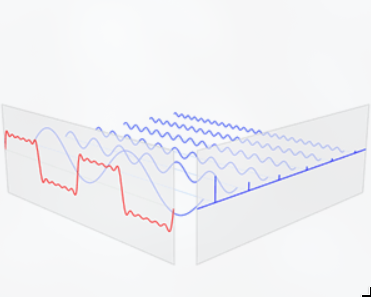
\includegraphics{images/04_01_IllustrazioneTrasformataFourier.png}
    \caption{Interpretazione della trasformata di Fourier}
    \label{fig:04_01_InterpretazioneTrasformataFourier}
\end{figure}

La figura~\ref{fig:04_01_InterpretazioneTrasformataFourier} fornisce una visualizzazione semplificata
di questa interpretazione: il risultato della trasformata è una funzione che \textbf{misura la similarità}
del segnale di ingresso con \textbf{segnali di riferimento a frequenze diverse}.
In particolare:
\begin{itemize}
    \item Se il segnale e l'esponenziale di prova sono \textbf{"simili"}, il prodotto scalare 
        restituisce un \textbf{valore elevato}.
    \item Al contrario, se \textbf{non condividono quella frequenza}, il loro prodotto tende 
        ad \textbf{annullarsi nel calcolo dell'area}.
\end{itemize}

Infine, siccome in generale $X(f) \in \mathbb{C}$, la \textbf{trasformata di un segnale}
presenta un \textbf{modulo} ed una \textbf{fase}. Vale la pena dare
un'interpretazione ad entrambe le componenti:
\begin{itemize}
    \item Il \textbf{modulo} indica \textit{"quanto" contributo} è dato 
        dalla \textit{specifica frequenza}.
    \item La \textbf{fase} indica \textit{"quando"} la specifica frequenza 
        \textit{si presenta nel segnale} (i.e. di \textit{quanto è sfasata rispetto a $t=0$}).
\end{itemize}

\section{Proprietà della trasformata}

Vediamo alcune proprietà della trasformata di Fourier:

\begin{prop}[PROPRIETA' DELLA TRASFORMATA]
    Le proprietà di nostro interesse sono:
    \begin{enumerate}
        \item \textbf{LINEARITA'} 
            \[
                \mathcal{F}[\alpha x_{1}(t) + \beta x_{2}(t)]=
                \alpha \mathcal{F}[x_{1}(t)] + \beta \mathcal{F}[x_{2}(t)]
            \]
        \item \textbf{CAMBIO DI SCALA}
            \[
                \begin{aligned}
                    x(t) &\overset{\mathcal{F}}{ \longrightarrow } X(f) \\ 
                    x(\alpha t) &\overset{\mathcal{F}}{ \longrightarrow } 
                    \frac{1}{|\alpha |}X \left( \frac{f}{|\alpha |} \right)
                \end{aligned}
            \]
        \item \textbf{TRASLAZIONE NEL TEMPO}
            \[
                \begin{aligned}
                    x(t) &\overset{\mathcal{F}}{ \longrightarrow } X(f) \\ 
                    x(t-t_{0}) &\overset{\mathcal{F}}{ \longrightarrow } X(f)e^{-j 2\pi ft_{0}}
                \end{aligned}
            \]
        \item \textbf{TRASLAZIONE IN FREQUENZA}
            \[
                \begin{aligned}
                    x(t) &\overset{\mathcal{F}}{ \longrightarrow } X(f) \\ 
                    x(t)e^{j 2\pi f_{0}t} &\overset{\mathcal{F}}{ \longrightarrow } X(f-f_{0})
                \end{aligned}
            \] 
        \item \textbf{MODULAZIONE} (derivabile dalla traslazione in frequenza) \\
            Con coseno:
            \[
                \begin{aligned}
                    x(t) &\overset{\mathcal{F}}{ \longrightarrow } X(f) \\ 
                    x(t)\cos (2\pi f_{0}t) &\overset{\mathcal{F}}{ \longrightarrow }
                    \frac{1}{2} [ X(f-f_{0}) + X(f+f_{0}) ]
                \end{aligned}
            \]
            Con seno:
            \[
                \begin{aligned}
                    x(t) &\overset{\mathcal{F}}{ \longrightarrow } X(f) \\ 
                    x(t)\sin (2\pi f_{0}t) &\overset{\mathcal{F}}{ \longrightarrow }
                    \frac{1}{2j} [ X(f-f_{0}) - X(f+f_{0}) ]
                \end{aligned}
            \]
        \item \textbf{CONVOLUZIONE}
            \[
                \begin{aligned}
                    x(t) \overset{\mathcal{F}}{ \longrightarrow } X(f) &\text{ , }
                    y(t) \overset{\mathcal{F}}{ \longrightarrow } Y(f) \\ 
                    x(t) \ast y(t) &\overset{\mathcal{F}}{ \longrightarrow } X(f)Y(f)
                \end{aligned}
            \]
        \item \textbf{SIMMETRIA HERMITIANA} Se $x(t)\in \mathbb{R}$, allora 
            $X(-f)=\overline{X(f)}$ (Per cui $\text{Re}[X(f)]$ è \textit{pari}, mentre
            $\text{Im}[X(f)]$ è \textit{dispari}). 
        \item \textbf{AREA DEL SEGNALE}
            \[
                \text{Area}[x(t)] = \int_{-\infty}^{+\infty} x(t) dt = 
                \int_{-\infty}^{+\infty} x(t) e^{-j 2\pi\cdot 0t}dt = X(0) 
            \]
            E, per simmetria, anche:
            \[
                \int_{-\infty}^{+\infty} X(f) df = \int_{-\infty}^{+\infty} X(f) e^{j 2\pi f\cdot 0} dt 
                = x(0)
            \] 
    \end{enumerate}
\end{prop}

\subsection{Esempi di calcolo}

Vediamo ora alcuni esempi di calcolo della trasformata per segnali notevoli.

Per cominciare, vediamo la \textbf{trasformata dell'impulso di Dirac}:

\begin{prop}[TRASFORMATA DELL'IMPULSO]
    Abbiamo:
    \[
        \mathcal{F}[\delta(t)] = 1
    \] 
\end{prop}

Infatti, per la \textit{proprietà rivelatrice dell'impulso}, abbiamo:
\[
    \int_{-\infty}^{+\infty} x(t)\delta(t-t_{0})dt = x(t_{0}) \\ \\
\] 
Per cui segue che:
\[
    \mathcal{F}[\delta(t)] = \int_{-\infty}^{+\infty} \delta(t-0) e^{-j 2\pi ft} dt
    = e^{-j 2 \pi ft}\bigg|_{t=0} = \cos(0) +j \sin(0) = 1
\]

Vediamo ora la trasformata dell'\textbf{esponenziale}:

\begin{prop}[TRASFORMATA DELL'ESPONENZIALE]
    Dato $x(t) = e^{j 2\pi f_{0}t}$, la sua trasformata è:
    \[
        \mathcal{F}\left[ e^{j 2\pi f_{0}t} \right] = \delta(f-f_{0})
    \]
\end{prop}

Questo risultato non deve stupirci: infatti, facendo appello all'interpretazione
che abbiamo dato alla trasformata come \textit{proiezione continua nel dominio della frequenza},
notiamo che un \textbf{segnale esponenziale} è \textbf{caratterizzato da una sola frequenza}, cioè
proprio $f_{0}$.

Inoltre, questo risultato implica anche:

\begin{prop}
    Di conseguenza, se $x(t)= 1 = e^{j 2\pi\cdot 0t}$, allora:
    \[
        \mathcal{F}[1] = \delta(f-0) = \delta(f)
    \] 
\end{prop}

Proseguiamo con la \textbf{trasformata del rettangolo}:

\begin{prop}[TRASFORMATA DEL RETTANGOLO]
    La trasformata di $x(t)=\text{rect}(t)$ è:
    \[
        X(f) = \frac{\sin \pi f}{\pi f} = \text{sinc}(f)
    \] 
\end{prop}

Infatti:
\[   
    \begin{aligned}
        X(f) &= \int_{-\infty}^{+\infty} \overbrace{\text{rect}(t)}^{=1} 
        e^{-j 2\pi ft}dt \\ 
             &= \int_{-\frac{1}{2}}^{\frac{1}{2}} e^{-j 2\pi ft}dt \\
             &= \frac{1}{-j 2\pi f} e^{-j 2\pi ft}\bigg|_{-\frac{1}{2}}^{\frac{1}{2}}
             = \frac{e^{j\pi f} - e^{-j\pi f}}{2j \pi f} \\
             &= \frac{\sin \pi f}{\pi f} = \text{sinc}(f)
    \end{aligned}
\]

\begin{remark}
    E' inoltre utile tenere a mente il fatto che vale anche:
    \[
        \mathcal{F}[\text{sinc}(t)] = \text{rect}(f)
    \] 
    Cioè $\text{sinc}$ e $\text{rect}$ sono \textbf{ciasuno la trasformata dell'altro}.
\end{remark}

Infine, per completezza, vediamo anche la seguente trasformata:

\begin{prop}[ESPONENZIALE NEGATIVO]
    Dato $x(t) = e^{-\alpha t}\mathbf{1}(t)$ (dove $\mathbf{1}(t)$ è il \textit{gradino unitario}
    e $\alpha\in \mathbb{R}^+$), la sua trasformata è:
    \[
        \mathcal{F}[x(t)] = \frac{1}{\alpha + j2\pi f}
    \] 
\end{prop}

Infatti:
\[
    \begin{aligned}
        X(f) &= \int_0^{+\infty} e^{-\alpha t} e^{-j 2\pi ft}dt \\ 
             &= \int_{0}^{+\infty} e^{-(\alpha + j2\pi f)t}dt \\ 
             &= \frac{-1}{\alpha + j 2\pi f} e^{-(\alpha + j 2\pi f)t}\bigg|_{0}^{+\infty} \\ 
             &= \frac{1}{\alpha + j 2\pi f}
    \end{aligned}
\]
Vediamo ora un esempio in cui sfruttiamo il cambio di scala:

\begin{exa}[CAMBIO DI SCALA]
    Consideriamo $x(t) = \text{rect}\left( \frac{t}{10} \right)$.
    Abbiamo semplicemente:
    \[
        X(f) = 10 \text{sinc}(10f)
    \] 
\end{exa}

Abbiamo ottenuto il risultato \textit{semplicemente applicando la proprietà}, senza
dover effettuare \textit{nessun calcolo}.

Vediamo anche degli esempi in cui possiamo sfruttare la traslazione in frequenza:

\begin{exa}[MODULAZIONE]
    Consideriamo un segnale del tipo $x(t)=\cos (2\pi f_{0}t)$. 
    Notiamo che possiamo scriverlo nella forma $x(t) = 1\cdot \cos (2\pi f_{0}t)$.
    Sfruttando la proprietà di \textbf{modulazione} abbiamo quindi:
    \[
        X(f) =\frac{1}{2}\delta(f-f_{0}) + \frac{1}{2}\delta(f+f_{0})
    \]
    Se consideriamo invece $x(t)=\sin (2\pi f_{0}t)$ abbiamo:
    \[
        X(f) = \frac{1}{2j}\delta(f-f_{0}) - \frac{1}{2j}\delta(f+f_{0})
    \] 
\end{exa}

Vediamo anche un esempio in cui \textit{applichiamo diverse proprietà insieme}:

\begin{exa}[ESEMPIO COMPOSTO]
    Consideriamo il segnale seguente:
    \[
        x(t) = \text{sinc}(10t) \cos(6\pi t)
    \] 
    Cominciamo col calcolare la trasformata di $x_{1}(t)=\text{sinc}(10t)$:
    \[
        \mathcal{F}[x_{1}(t)] = \frac{1}{10} \text{rect} \left( \frac{f}{10} \right)
    \] 
    Infine, applicando la proprietà di modulazione a $x_{1}$ con 
    $\cos (6\pi t)=\cos (2\pi\cdot 3t)$ troviamo:
    \[
        \begin{aligned}
            \mathcal{F}[x(t)] &= \frac{1}{2} \left[ 
                \frac{1}{10}\text{rect} \left( \frac{f-3}{10} \right) +
                \frac{1}{10}\text{rect} \left( \frac{f+3}{10} \right)
            \right] \\ 
            &= \frac{1}{20}\text{rect} \left( \frac{f-3}{10} \right) +
            \frac{1}{20}\text{rect} \left( \frac{f+3}{10} \right)
        \end{aligned}
    \] 
\end{exa}

\section{Trasformata e sistemi LTI}

Una proprietà particolarmente utile è quella che riguarda la convoluzione: infatti, se
abbiamo un \textbf{LTI} con un \textbf{segnale di ingresso} $x(t)$, possiamo \textbf{calcolare
la sua uscita} nel \textbf{dominio della frequenza} con \textbf{facilità}, come mostrato nella
figura~\ref{fig:04_02_ConvoluzioneDomTrasformata}.

\begin{figure}[!ht]
    \centering
    \begin{tikzpicture}[
        >=Stealth, 
        thick, 
        font=\sffamily,
        block/.style={
            draw=nord10, 
            rectangle, 
            minimum width=2.5cm, 
            minimum height=1cm, 
            align=center,
            text=nord0
        },
        arrow/.style={->, nord0},
        label/.style={text=nord0, font=\small}
        ]

        % ==========================================
        % PARTE SUPERIORE: DOMINIO DEL TEMPO
        % ==========================================

        % Nodi principali
        \node (xt) at (-4, 2) {\(x(t)\)};
        \node[block] (h) at (0, 2) {\(h(t)\)};
        \node (yt) at (2.65, 2) {\(y(t)\)};
        \node (eq_t) at (4.2, 2) {\(= x(t) * h(t)\)};

        % Frecce
        \draw[arrow] (xt) -- (h);
        \draw[arrow] (h) -- (yt);

        % Annotazioni
        \node[label, above] at (-2.5, 2) {LTI};

        % ==========================================
        % TRASFORMAZIONE DI FOURIER
        % ==========================================

        % Freccia verso il basso
        \draw[arrow, nord11] (0, 1.5) -- (0, -1.5);
        \node[nord11, font=\large\bfseries] at (-0.3, 0) {\(\mathcal{F}\)};

        % ==========================================
        % PARTE INFERIORE: DOMINIO DELLA FREQUENZA
        % ==========================================

        % Nodi principali
        \node (Xf) at (-4, -2) {\(X(f)\)};
        \node[block] (H) at (0, -2) {\(H(f)\)};
        \node (Yf) at (2.65, -2) {\(Y(f)\)};
        \node (eq_f) at (4.5, -2) {\(= H(f) \cdot X(f)\)};

        % Frecce
        \draw[arrow] (Xf) -- (H);
        \draw[arrow] (H) -- (Yf);

    \end{tikzpicture}
    \caption{Sistemi LTI nel dominio della trasformata}
    \label{fig:04_02_ConvoluzioneDomTrasformata}
\end{figure}

Vediamo anche un esempio in cui l'applicazione della proprietà sulla convoluzione
semplifica di molto i calcoli: immaginiamo di voler calcolare la 
\textbf{trasformata del triangolo}. Sappiamo che il triangolo è il risultato della 
\textbf{convoluzione tra due rect}, per cui:
\[
    \text{triang}(t) = \text{rect}(t) \ast \text{rect}(t)
\]

Possiamo allora calcolarne la trasformata come segue:

\begin{exa}[TRASFORMATA DEL TRIANGOLO]
    \[
        \mathcal{F}[\text{triang}(t)] = \mathcal{F}[\text{rect}(t) \ast \text{rect}(t)]
        = \text{sinc}^2(f)
    \] 
\end{exa}

Inoltre, ricordando la relazione tra l'\textbf{area del segnale} e la \textbf{sua trasformata}, 
abbiamo anche:
\[
    \begin{aligned}
        z(t) &= x(t) \ast y(t) \\ 
        \text{Area}[z(t)] &= Z(0) \\ 
                      &= X(f) Y(f) \bigg|_{f=0} \\ 
                      &= X(0) Y(0)
    \end{aligned}
\]

\subsection{Risposta in frequenza}

Possiamo sfruttare la trasformata di Fourier per studiare i sistemi nel 
\textbf{dominio della frequenza invece che nel dominio del tempo}.

\begin{remark}[RISPOSTA IN FREQUENZA]
    Quando l'analisi viene fatta nel \textit{dominio della trasformata di Fourier}
    si parla di \textbf{analisi in frequenza} e \textbf{risposta in frequenza}
    del sistema (cioè la \textit{trasformata} di $h(t)$, ovvero $H(f)$).
\end{remark}

Vediamo alcuni esempi per capire di cosa si tratta.

Consideriamo un generico sistema \textbf{LTI} caratterizzato da una 
\textbf{risposta impulsiva} $h(t)$, come mostrato in figura~\ref{fig:04_03_EsSistemaLTI}.

\begin{figure}[!ht]
    \centering
    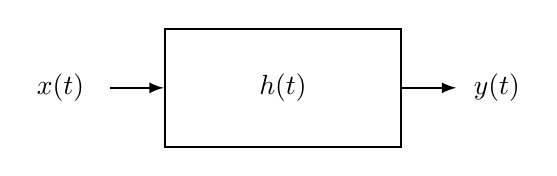
\begin{tikzpicture}[>=latex]
        \node[draw, thick, minimum width=3cm, minimum height=1.5cm] (lti) at (0,0) {$h(t)$};
        \draw[->, thick] (-2.2, 0) -- (lti.west);
        \node[anchor=east] at (-2.4, 0) {$x(t)$};
        \draw[->, thick] (lti.east) -- (2.2, 0);
        \node[anchor=west] at (2.3, 0) {$y(t)$};
    \end{tikzpicture}
    \caption{Esempio di sistema LTI}
    \label{fig:04_03_EsSistemaLTI}
\end{figure}

Per cominciare, consideriamo un ingresso dato da un \textbf{segnale esponenziale}:
\[
    x(t) = e^{j 2\pi f_{0}t}
\]
Calcoliamo l'\textbf{uscita del sistema} nel \textbf{dominio della frequenza}:
\[
    \begin{aligned}
        Y(f) &= H(f) X(f) \\ 
             &= H(f) \delta(f-f_{0})
    \end{aligned}
\]

Ora, per la \textit{proprietà rivelatrice} dell'impulso, abbiamo:
\[
    Y(f) = H(f_{0})\delta(f-f_{0})
\]
Dove $H(f_{0})$ è un \textit{numero (complesso)}. Per cui, applicando l'\textbf{antitrasformata} per 
\textbf{tornare al dominio del tempo}, concludiamo che:
\[
    y(t) = H(f_{0}) e^{j 2\pi f_{0}t}
\]
Notiamo che l'\textbf{uscita del sistema} è semplicemente l'\textbf{ingresso riscalato}
di un fattore $H(f_{0})$.

\begin{remark}[AUTOFUNZIONE PER SISTEMI LTI]
    "Applicare" un \textbf{sistema LTI} $T_h$ ad un \textbf{segnale esponenziale} $x(t)$ è 
    \textbf{equivalente} a \textbf{riscalare il segnale}:
    \[
        T_h \{x(t)\} = \lambda x(t) \text{ , } \lambda = H(f_{0})
    \] 
    Possiamo quindi concludere che tali segnali sono le \textbf{autofunzioni dei sistemi LTI}
    (analoghi agli \textit{autovettori} per le matrici) associati all'
    \textbf{autovalore complesso} $H(f_{0})$.
\end{remark}

Vediamo ora cosa succede se consideriamo lo \textit{stesso sistema LTI}, ma con un
\textbf{ingresso} $x(t)$ \textbf{sinusoidale}:
\[
    x(t) = A \cos(2\pi f_{0}t + \varphi )
\] 

Per cominciare, riscriviamo il segnale di ingresso come segue:
\[
    \begin{aligned}
        x(t) &=\frac{A}{2} e^{j(2\pi f_{0}t + \varphi )} + \frac{A}{2} e^{-j(2\pi f_{0}t + \varphi )} \\ 
             &=\frac{A}{2} e^{j \varphi } e^{j 2\pi f_{0}t} + \frac{A}{2} e^{-j \varphi } e^{-j 2\pi f_{0}t}
    \end{aligned}
\]
Così facendo abbiamo messo in evidenza il fatto che possiamo vederli come \textbf{segnali costanti} 
$\frac{A}{2} e^{j \varphi}$ e $\frac{A}{2} e^{-j \varphi}$ \textbf{traslati} di 
$e^{j 2\pi f_{0} t}$ e $e^{-j 2\pi f_{0} t}$. La trasformata risulta quindi essere:
\[
    X(f) = \frac{A}{2} e^{j \varphi } \delta(f-f_{0}) + \frac{A}{2} e^{-j \varphi } \delta(f+f_{0})
\]

Allora la risposta del sistema è:
\[
    \begin{aligned}
        Y(f) = H(f)X(f) &= \frac{A}{2} H(f) e^{j \varphi } \delta(f-f_{0}) + 
                \frac{A}{2} H(f) e^{-j \varphi } \delta(f+f_{0}) \\ 
             &= \frac{Ae^{j \varphi }}{2} H(f_{0})\delta(f-f_{0}) +
                \frac{Ae^{-j \varphi }}{2} H(-f_{0})\delta(f+f_{0})
    \end{aligned}
\]

Essendo il \textit{segnale reale}, è utile ricordare che la sua trasformata gode di
\textit{simmetria Hermitiana}, per cui $H(-f_{0})=\overline{H(f)}$ e la risposta risulta:
\[
   Y(f) = \frac{Ae^{j \varphi }}{2} H(f_{0})\delta(f-f_{0}) +
          \frac{Ae^{-j \varphi }}{2} \overline{H(f_{0})}\delta(f+f_{0}) 
\]
Ricordando che $H(f_{0})$ è un \textbf{numero complesso}, scriviamo:
\[
    Y(f) = \frac{Ae^{j \varphi }}{2} |H(f_{0})|e^{j\angle H(f_{0})} \delta(f-f_{0}) +
          \frac{Ae^{-j \varphi }}{2} |H(f_{0})|e^{-j\angle H(f_{0})} \delta(f+f_{0}) 
\]
Raccogliendo troviamo:
\[
    Y(f) = \frac{A|H(f_{0})|}{2} \left[ e^{j(\varphi + \angle H(f_0)) } \delta(f-f_{0}) +  
           e^{-j (\varphi + \angle H(f_0)) } \delta(f+f_{0}) \right]
\]

Ora, antitrasformando per \textit{tornare nel dominio del tempo}, troviamo:
\[
    \begin{aligned}
        y(t) &= \frac{A|H(f_{0})|}{2} \left[ e^{j(\varphi + \angle H(f_0))} e^{j 2\pi f_{0}t} +
                e^{-j(\varphi + \angle H(f_0))} e^{-j 2\pi f_{0}t} \right] \\ \\
             &= \frac{A|H(f_{0})|}{2} \underbrace{ \left[ e^{j(2\pi f_{0}t + \varphi + \angle H(f_0))} +
             e^{-j(2\pi f_{0}t + \varphi + \angle H(f_0))} \right] }_{=2\cos 
                (2\pi f_{0}t + \varphi + \angle H(f_0) )} \\ \\
             &= A|H(f_{0})| \cos (2\pi f_{0}t + \varphi + \angle H(f_0) )
    \end{aligned}
\]

\begin{remark}[RISPOSTA SISTEMI LTI A INGRESSI SINUSOIDALI]
    La \textbf{risposta} di un \textbf{sistema LTI} ad un \textbf{ingresso sinusoidale}
    di \textbf{frequenza} $f_{0}$ è un altro \textbf{segnale sinusoidale}, con 
    la \textbf{stessa frequenza}, ma \textbf{modulo} e \textbf{fase modificati}:
    \begin{itemize}
        \item Il \textbf{modulo} è \textbf{scalato} di un fattore $|H(f_{0})|$.
        \item Alla \textbf{fase} è  sommato un contributo dato da $\angle H(f_{0})$.
    \end{itemize}
\end{remark}

Infine, dato che in generale $Y(f)\in \mathbb{C}$, essa può presentare una 
\textbf{fase}, che merita di essere discussa.
In particolare, è utile definire la seguente quantità:

\begin{definition}[RITARDO DI GRUPPO]
    Il \textbf{ritardo di gruppo} è il \textbf{ritardo subito} dal 
    \textbf{segnale} al \textbf{variare delle frequenze che lo compongono}:
    \[
        \tau_g(f) \coloneqq -\frac{1}{2\pi} \frac{d}{df} \angle Y(f)
    \] 
\end{definition}

Questa quantità è importante perchè:

\begin{remark}[RITARDO DI GRUPPO E DISTORSIONE]
    Se il ritardo di gruppo è \textbf{costante} su 
    \textbf{al variare della frequenza del segnale}, possiamo concludere
    che \textbf{il sistema non ha introdotto una distorsione}, cioè ha 
    \textbf{preservato la forma} del segnale.

    Al contrario, se \textbf{varia con la frequenza}, si verifica una 
    \textbf{distorsione della forma d'onda} a causa della 
    \textbf{diversa velocità di propagazione} 
    delle \textbf{diverse componenti frequenziali}.
\end{remark}

\subsection{Banda e larghezza di banda}

Dato un segnale, possiamo definire la sua \textbf{banda}:

\begin{definition}[BANDA DI UN SEGNALE]
    La banda di un segnale $x(t)$ è l'
    \textbf{intervallo di frequenze non negative} 
    per cui la sua \textbf{trasformata} risulta \textbf{non nulla}:
    \[
        \mathcal{B}_x \coloneqq \{f\in \mathbb{R}^+\}   : X(f) \ne 0 
    \] 
\end{definition}

E' da notare che consideriamo \textbf{solo le frequenze positive}. Questo perchè,
come abbiamo visto, se il segnale è reale sappiamo che $X(-f) = \overline{X(f)}$,
quindi la \textbf{parte reale della trasformata è pari} e ci \textit{basta considerare
le frequenze positive} (lo \textit{spettro negativo sarà uguale}).

Inoltre, possiamo anche \textit{estendere questo concetto ai sistemi}:

\begin{definition}[BANDA DI UN SISTEMA]
    Dato un \textbf{sistema} $h$, ne definiamo la \textbf{banda passante} $B_h$
    a partire dalla \textbf{risposta in frequenza}:
    \[
        \mathcal{B}_h = \{f\in \mathbb{R}^+ : H(f) \ne 0 \}
    \] 
\end{definition}

Si definisce inoltre la \textbf{larghezza di banda}:

\begin{definition}[LARGHEZZA DI BANDA]
    Data la \textbf{banda} di un segnale (o la \textit{banda passante di un sistema})
    $\mathcal{B}= [f_{1},f_{2}]  $, la \textbf{larghezza di banda} $B$ 
    (o \textit{bandwidth}) è:
    \[
        B = f_{2} - f_{1}
    \] 
\end{definition}

La figura~\ref{fig:04_04_EsempioBandaLarghezza} mostra la \textbf{banda} e la 
\textbf{larghezza di banda} per un segnale di esempio.

\begin{figure}[!ht]
    \centering
    \begin{tikzpicture}[xscale=1.5, yscale=2, >=stealth, font=\small]
        % Assi
        \draw[->, thick, nord0] (-4, 0) -- (4.5, 0) node[right, font=\bfseries] {\(f\)};
        \draw[->, thick, nord0] (0, -0.2) -- (0, 1.5) node[above, font=\bfseries] {\(X(f)\)};

        % Spettro del segnale (esempio di un passa-banda)
        % Parte positiva (quella che definisce la banda)
        \draw[very thick, nord10] (1, 0) -- (1, 1) -- (3, 1) -- (3, 0);
        % Parte negativa (simmetrica, tratteggiata per far capire che non la contiamo)
        \draw[very thick, nord10, dashed] (-3, 0) -- (-3, 1) -- (-1, 1) -- (-1, 0);

        % Evidenziazione della Banda (Area sotto la parte positiva)
        \fill[nord14, opacity=0.3] (1, 0) rectangle (3, 1);

        % Etichette sugli assi
        \draw[nord0, thick] (0.95, 0) -- (1.05, 0) node[below=2pt, nord0] {\(f_1\)};
        \draw[nord0, thick] (2.95, 0) -- (3.05, 0) node[below=2pt, nord0] {\(f_2\)};
        \draw[nord0, thick] (0, 1) -- (-0.05, 1) node[left, nord0] {\(\max\)};

        % Parentesi graffa per la Banda B_x
        \draw[decorate, decoration={brace, amplitude=5pt, mirror}, nord11, thick] 
            (1, -0.4) -- (3, -0.4) node[midway, below=6pt, nord11] 
            {Banda \(B_x = \{f \in \mathbb{R}^+ : X(f) \neq 0\}\)};

        % Frecce per la Larghezza di Banda
        \draw[<->, thick, nord12] (1, 1.2) -- (3, 1.2) 
            node[midway, above, nord12] {Larghezza di banda \(B = f_2 - f_1\)};

        % Nota sulla parte negativa
        \node[align=center, font=\footnotesize, nord3] at (-2, 0.5) 
            {Spettro negativo \\ simmetrico};
    \end{tikzpicture}
    \caption{Esempio: banda e larghezza di banda di $x(t) = \text{sinc}(t) e^{j 2\pi f_{0}t}$}
    \label{fig:04_04_EsempioBandaLarghezza}
\end{figure}

A questo punto, è importante notare che in moltissimi casi la definizione di banda 
come \textit{intervallo in cui la trasformata è diversa da zero} 
porterebbe ad avere una \textbf{banda infinita}, mentre dal \textit{punto di vista pratico} 
quello che interessa è l’\textbf{intervallo in cui la trasformata è \textit{significativamente}
diversa da zero}.

Con questo in mente, consideriamo due \textbf{definizioni alternative}
di \textbf{larghezza di banda}:

\begin{definition}[LARGHEZZA DI BANDA - DEF. ALTERNATIVE]
    Consideriamo le seguenti due definizioni:
    \begin{enumerate}
        \item \textbf{Primo zero}: ci limitiamo al \textit{primo zero della trasformata}.
            \[
                B = \text{min } \{ f > 0 \text{ t.c } H(f) = 0 \}  
            \] 
        \item Basata sull'\textbf{ampiezza} (in \textit{decibel}):
            \[
                B = \text{min } \left\{ f > 0 \text{ t.c. } \left| \frac{H(f)}{H(0)} \right| 
                = 10^{- \frac{A}{20}} \right\}
            \] 
    \end{enumerate}
\end{definition}

Per quanto riguarda la seconda definizione, ricordiamo la \textit{definizione di decibel}
e consideriamo la figura~\ref{fig:04_05_EsempioDefPraticaBanda} per un esempio visivo.

\begin{figure}[!ht]
    \centering
    \begin{tikzpicture}
        \begin{axis}[
            width=12cm, height=7.5cm,
            xmin=0, xmax=2,
            ymin=-100, ymax=5,
            xtick={0, 0.2, 0.4, 0.6, 0.8, 1, 1.2, 1.4, 1.6, 1.8, 2},
            ytick={0, -10, -20, -30, -40, -50, -60, -70, -80, -90, -100},
            xlabel={\(f\) (Hz)},
            ylabel={\(|H(f)|\) (dB)},
            axis line style={nord0, thick},
            tick style={nord0, thick},
            tick label style={nord0},
            label style={nord0, font=\bfseries},
            grid=major,
            grid style={nord4, dashed},
            clip=false
            ]

            % --- 1. Curva della risposta in frequenza (approssimata per riprodurre la forma) ---
            \addplot [
                nord10, very thick, smooth
                ] coordinates {
                    (0, 0) (0.1, 0) (0.2, 0) (0.3, 0) (0.35, -0.1)
                    (0.4, -0.5) (0.45, -1.2) (0.5, -3) 
                    (0.55, -8) (0.6, -25) (0.652, -30) 
                    (0.68, -35) (0.75, -38) (0.82, -45) (0.85, -40) 
                    (0.87, -40) (0.9, -45) (1.0, -55) (1.05, -60) 
                    (1.1, -55) (1.2, -60) (1.25, -70) 
                    (1.3, -60) (1.4, -65) (1.45, -90) 
                    (1.5, -65) (1.62, -50) (1.7, -100)
                };

            % --- 2. Linee orizzontali e verticali per le larghezze di banda ---

            % Banda a 3 dB (B_3dB)
            \draw[dashed, nord3, thick] (axis cs:0, -3) -- (axis cs:0.5, -3);
            \draw[dashed, nord3, thick] (axis cs:0.5, -3) -- (axis cs:0.5, -101);

            % Banda a 40 dB (B_40dB)
            \draw[dashed, nord3, thick] (axis cs:0, -40) -- (axis cs:0.77, -40);
            \draw[dashed, nord3, thick] (axis cs:0.77, -40) -- (axis cs:0.77, -101);

            % Banda a 60 dB (B_60dB)
            \draw[dashed, nord3, thick] (axis cs:0, -60) -- (axis cs:1.05, -60);
            \draw[dashed, nord3, thick] (axis cs:1.05, -60) -- (axis cs:1.05, -101);

            % --- 3. Etichette testuali ---

            % Etichette in alto a sinistra
            \node[anchor=north, nord0, font=\footnotesize] at (axis cs:0.2, -3) {\(B_{3dB}\)};
            \node[anchor=north, nord0, font=\footnotesize] at (axis cs:0.2, -40) {\(B_{40dB}\)};
            \node[anchor=north, nord0, font=\footnotesize] at (axis cs:0.2, -60) {\(B_{60dB}\)};

        \end{axis}

    \end{tikzpicture}
    \caption{Larghezza di banda basata sull'attenuazione dell'ampiezza}
    \label{fig:04_05_EsempioDefPraticaBanda}
\end{figure}

\begin{remark}
    Il \textbf{decibel} è utilizzato per quantificare l'\textbf{attenuazione} 
    del segnale ed è definito come:
    \[
        A_{dB} = 20 \log_{10} \left( \frac{|H(f)|}{H(0)} \right)
    \] 
    Spesso si usano come valori di $A$:
    \begin{itemize}
        \item $A=3dB$: valore di \textbf{half-power} (si ha $10^{-3/20} \approx 1/\sqrt{2}$)
        \item $A=40dB$: attenuazione dell'ampiezza di $100$ volte.
        \item $A=60dB$: attenuazione dell'ampiezza di $1000$ volte.
    \end{itemize}
\end{remark}


\section{Teorema di Parseval}

Un teorema particolarmente importante è il seguente:

\begin{theorem}[TEOREMA DI PARSEVAL]
    Dati due \textbf{segnali} $x(t)$ e $y(t)$, vale:
    \[
        \int_{-\infty}^{+\infty} x(t) \overline{y(t)} dt = 
        \int_{-\infty}^{+\infty} X(f) \overline{Y(f)} df  
    \] 
\end{theorem}

Vediamo un esempio in cui questo teorema può risultare utile:

\begin{exa}[APPLICAZIONE TH. PARSEVAL]
    Consideriamo:
    \[
        \begin{aligned}
            x(t) = \text{sinc}(10t) & & y(t) = \text{sinc}(5t)
        \end{aligned}
    \] 
    L'integrale seguente è particolarmente complicato da calcolare:
    \[
        \int_{-\infty}^{+\infty} \frac{\sin 10\pi t}{10\pi t} \frac{\sin 5\pi t}{5\pi t} dt
    \] 
    Possiamo tuttavia sfruttare il teorema di Parseval per calcolare:
    \[
        \begin{aligned}
            \int_{-\infty}^{+\infty} X(f) \overline{Y(f)} df &= 
            \frac{1}{50} \int_{-\infty}^{+\infty} \text{rect} \left( \frac{f}{10} \right)
            \overline{ \text{rect} \left( \frac{f}{5} \right) } df \\ 
            &= \frac{1}{50} \int_{-\infty}^{+\infty} \text{rect} \left( \frac{f}{10} \right)
            \text{rect} \left( \frac{f}{5} \right) df \\ 
            &= \frac{1}{50} \int_{-\infty}^{+\infty} \text{rect} \left( \frac{f}{5} \right) \\ 
            &= \frac{5}{50} = \frac{1}{10}
        \end{aligned}
    \] 
    Dove abbiamo sfruttato il fatto che:
    \begin{itemize}
        \item Il \textbf{congiugato} di un segnale \textbf{reale} 
            rimane il \textbf{segnale stesso}.
        \item La \textbf{moltiplicazione di due rect} risulta in un \textbf{rect}
            nella \textbf{zona di intersezione} fra i due.
    \end{itemize}
\end{exa}

Inoltre osserviamo che, se $y(t) = x(t)$, dal teorema segue che:

\begin{prop}[COROLLARIO TH. PARSEVAL]
    \[
        \int_{-\infty}^{+\infty} x(t) \overline{x(t)} dt = 
        \int_{-\infty}^{+\infty} |x(t)|^2 dt =
        \int_{-\infty}^{+\infty} X(f) \overline{X(f)} df =
        \int_{-\infty}^{+\infty} |X(f)|^2 df
    \] 
\end{prop}

\section{Trasformata di Fourier a tempo discreto}

Vediamo ora come possiamo \textit{generalizzare la trasformata di Fourier} per 
poterla \textbf{applicare} anche a \textbf{segnali a tempo discreto}.

\begin{definition}[TRASFORMATA DI FOURIER A TEMPO DISCRETO]
    Dato un \textbf{segnale} $x(nT)$ ($n\in \mathbb{Z}$) a \textbf{tempo discreto}, la sua
    \textbf{trasformata di Fourier} $\mathcal{F}[x(nT)]$ è definita come segue:
    \[
        \mathcal{F}[x(nT)] = X(f) = \sum_{n=-\infty}^{+\infty} T x(nT) e^{-j 2\pi fnT}
    \] 
\end{definition}

\begin{remark}[CONTINUITA' DELLA FREQUENZA]
    Anche se il segnale originale era in tempo discreto, la sua trasformata
    è \textbf{comunque in frequenze continue} $f\in \mathbb{R}$.
\end{remark}

Ora espandiamo la sommatoria per notare un particolare:
\[
    \begin{aligned}
        X(f) = \ldots +& \underbrace{ Tx(-2T) e^{j 2\pi f\cdot 2T} }_{n=-2} + 
                  \underbrace{ Tx(-T) e^{j 2\pi f\cdot T} }_{n=-1}
                 + Tx(0) \\ 
                 +& \underbrace{ Tx(T) e^{-j 2\pi f\cdot T} }_{n=1} + 
                  \underbrace{ Tx(2T) e^{-j 2\pi f\cdot 2T} }_{n=2} + \ldots 
    \end{aligned}
\]

Notiamo che:
\begin{itemize}
    \item I termini associati ad $n= \pm 1$ sono \textbf{periodici} di periodo $T_{1} = \frac{1}{T}$.
    \item I termini associati ad $n= \pm 2$ sono \textbf{periodici} di periodo $T_{2} = \frac{1}{2T}$.
\end{itemize}

Andando avanti, noteremmo che, in generale, i termini associati ad $n= \pm k$ sono 
\textbf{periodici} di periodo $T_{k} = \frac{1}{kT}$. La cosa importante è che
\textbf{tutti questi termini} si \textbf{ripetono} con \textbf{periodo comune} $\frac{1}{T}$.

Vale quindi il seguente fatto (\textbf{solo per la trasformata a
tempo discreto}, non era vero per quella a tempo continuo):

\begin{remark}[PERIODICITA']
    Per segnali a \textbf{tempo discreto}, la \textbf{trasformata} di Fourier 
    risulta essere \textbf{periodica} di \textit{periodo}:
    \[
        T_f = \frac{1}{T}
    \] 
\end{remark}

Inoltre, anche a tempo discreto possiamo definire la trasformata inversa:

\begin{definition}[TRASFORMATA INVERSA A TEMPO DISCRETO]
    Il segnale \textit{"originale"} può essere ottenuto con la trasformazione inversa:
    \[
        x(nT) = \int_{- \frac{1}{2T}}^{\frac{1}{2T}} X(f) e^{j 2\pi fnT} df
    \] 
\end{definition}

E' da notare che:

\begin{remark}
    Essendo $X(f)$ \textbf{periodica} per un segnale discreto, possiamo \textbf{ricostruire}
    il \textbf{segnale originale} $x(nT)$ \textbf{integrando} su 
    \textbf{un solo periodo} $T_f$.

    In generale, avremmo potuto scegliere \textit{qualsiasi intervallo} di 
    \textit{ampiezza} $T_f$ (e.g. $[0, \frac{1}{T}]$); quello scelto nella 
    defininizione è \textit{più comune} data la sua \textit{simmetria rispetto
    all'origine}.
\end{remark}

\subsection{Esempi di calcolo}

Vediamo ora alcuni esempi:

Per cominciare, consideriamo il segnale:
\[
    x(nT) = \text{rect} \left(\frac{nT}{5T} \right)
\]

Essendo $\text{rect}(t)$ definito se $|t|\le \frac{1}{2}$, abbiamo:
\[
    x(nT) = \begin{cases}
        1 & |n| \le 2 \\ 
        0 & |n| > 2
    \end{cases}
\]

Il segnale è mostrato in figura:

\begin{figure}[!ht]
    \centering
    \begin{tikzpicture}[>=stealth, font=\small]

        % Assi cartesiani
        \draw[->, thick, nord0] (-4.5, 0) -- (4.5, 0) node[right, font=\bfseries] {\(nT\)};
        \draw[->, thick, nord0] (0, -0.2) -- (0, 1.3) node[above, font=\bfseries] {\(x(nT)\)};

        % Linea tratteggiata di guida per y=1
        \draw[dashed, nord3, thick] (-2.5, 1) -- (2.5, 1);

        % Steli e punti per n dove x(nT) = 1 (da -2 a 2)
        \foreach \x in {-2, -1, 0, 1, 2} {
            \draw[nord8, very thick] (\x, 0) -- (\x, 1);
            \fill[nord10] (\x, 1) circle (2.5pt);
        }

        % Punti per n dove x(nT) = 0 (fuori dall'intervallo)
        \foreach \x in {-4, -3, 3, 4} {
            \fill[nord10] (\x, 0) circle (2.5pt);
        }

        % Etichette sull'asse x (nT)
        \foreach \x in {-4, -3, -2, -1, 1, 2, 3, 4} {
            \draw[nord0, thick] (\x, 0) -- (\x, -0.05) node[below, nord0] {\(\frac{\x}{5}\)};
        }
        \draw[nord0, thick] (0, 0) -- (0, -0.05) node[below, nord0] {\(0\)};
        
        % Etichetta sull'asse y
        \draw[nord0, thick] (0, 1) -- (-0.05, 1) node[left, nord0] {\(1\)};

        % Parentesi graffa per evidenziare l'intervallo |n| <= 2
        \draw[decorate, decoration={brace, amplitude=5pt, mirror}, nord11, thick] 
            (-2, -0.75) -- (2, -0.75) node[midway, below=6pt, nord11] {\(|n| \le 2\)};

    \end{tikzpicture}
    \caption{Esempio di segnale rect a tempo discreto}
\end{figure}

Calcoliamone la trasformata:
\[
    \begin{aligned}
        X(f) =& T e^{-j 2\pi f\cdot (-2T)} + 
                T e^{-j 2\pi f\cdot (-T)} + 
                T \\ 
             +& T e^{-j 2\pi f\cdot T} + 
                T e^{-j 2\pi f\cdot 2T)} 
    \end{aligned}
\]

Raccogliendo i termini troviamo:
\[
    \begin{aligned}
        X(f) = T \big[ 1 + &\left( e^{j 2\pi f\cdot 2T} + e^{-j 2\pi f\cdot 2T} \right) \\ 
                        &\left( e^{j 2\pi f\cdot T} + e^{-j 2\pi f\cdot T} \right) \big]
    \end{aligned}
\]

Per cui concludiamo:
\[
    X(f) = T\left[ 1 + 2\cos(2\pi fT) + 2\cos(4\pi fT)  \right]
\]

E' facile intuire che il risultato generale è:

\begin{prop}[TRASFORMATA DEL RECT A T.D.]
    In \textbf{generale}, la trasformata di un segnale rect del tipo
    \[
        x(nT) = \text{rect} \left( \frac{nT}{LT} \right)
    \] 
    Con $L=2M+1$, $M\in \mathbb{N}$, è:
    \[
        X(f) = T \left[ 1 + 2 \sum_{n=1}^M \cos(2\pi fnT) \right]
    \] 
\end{prop}

Consideriamo ora $x(nT) = \left( \frac{1}{3} \right)^{nT} \mathbf{1}(nT)$, mostrato
anche in figura:

\begin{figure}[!ht]
    \centering
    \begin{tikzpicture}[>=stealth, font=\small]

        % Assi cartesiani
        \draw[->, thick, nord0] (-2.5, 0) -- (5.5, 0) node[right, font=\bfseries] {\(nT\)};
        \draw[->, thick, nord0] (0, -0.1) -- (0, 1.4) node[above, font=\bfseries] {\(x(nT)\)};

        % Steli e punti per n >= 0 (valori calcolati: 1, 1/3, 1/9, 1/27, 1/81)
        \foreach \n/\val in {0/1, 1/0.333, 2/0.111, 3/0.037, 4/0.012} {
            \draw[nord8, very thick] (\n, 0) -- (\n, \val);
            \fill[nord10] (\n, \val) circle (2.5pt);
        }

        % Punti per n < 0 (dove 1(nT) = 0)
        \foreach \n in {-1, -2} {
            \fill[nord10] (\n, 0) circle (2.5pt);
        }

        % Etichette sull'asse x (nT)
        \foreach \x/\label in {-2/-2T, -1/-T, 0/0, 1/T, 2/2T, 3/3T, 4/4T} {
            \draw[nord0, thick] (\x, 0) -- (\x, -0.05) node[below, nord0] {\(\label\)};
        }

        % Etichette sull'asse y
        \draw[nord0, thick] (0, 1) -- (-0.05, 1) node[left, nord0] {\(1\)};
    \end{tikzpicture}
    \caption{Esempio di sequenza esponenziale}
\end{figure}

Applicando la trasformata, troviamo $X(f)=0$ per $n<0$, mentre per $n\ge 0$ abbiamo:
\[
    X(f) = \sum_{n=0}^{+\infty} \left( \frac{1}{3} \right)^n e^{-j 2\pi fnT}
\]

Riscriviamolo nella forma:
\[
    X(f) = \sum_{n=0}^{+\infty} \left( \frac{1}{3} e^{-j 2\pi fT} \right)^n
\]

Essendo questa una \textbf{serie geometrica} di ragione $r=\frac{1}{3} e^{-j 2\pi fT}$ 
con $|r|<1$, troviamo che la serie converge a:
\[
    X(f) = \frac{1}{1 - \frac{1}{3}e^{-j 2\pi fT} }
\]

A questo punto è facile intuire il \textbf{risultato generale} per 
una sequenza esponenziale generica:

\begin{prop}[TRASFORMATA DELLA SEQUENZA ESPONENZIALE]
    In generale, la trasformata di $x(nT) = a^{nT} \mathbf{1}(nT)$
    \[
        X(f) = \frac{1}{1 - ae^{-j 2\pi fT} } \text{ , }|a|<1
    \] 
\end{prop}

% ------------------------------------------------------------------------------------
%                               CAMPIONAMENTO
% ------------------------------------------------------------------------------------
\chapter{Campionamento}

Abbiamo fin'ora considerato sistemi  in cui \textbf{ingresso} e \textbf{uscita}
sono \textbf{entrambi} a \textbf{tempo continuo} (o \textit{entrambi a tempo discreto}).

Consideriamo ora invece dei sistemi in cui l'\textbf{ingresso} è un
\textbf{segnale a tempo continuo}, mentre l'\textbf{uscita} è un
\textbf{segnale a tempo discreto}, come in figura:

\begin{figure}[!ht]
    \centering
    \begin{tikzpicture}[>=latex, font=\small, scale=0.9]

        % Blocco principale (leggermente ingrandito per far stare l'interruttore)
        \node[draw, thick, nord0, minimum width=3.5cm, minimum height=1.8cm] (lti) at (0,0) {};

        % Fili interni al blocco
        \draw[thick, nord0] (-1.3, 0) -- (-0.4, 0); % Filo sinistro
        \draw[thick, nord0] (0.4, 0) -- (1.3, 0);   % Filo destro

        % Punti di contatto dell'interruttore
        \fill[nord10] (-0.4, 0) circle (1.8pt);
        \fill[nord10] (0.4, 0) circle (1.8pt);

        % Braccio dell'interruttore (aperto)
        \draw[thick, nord10] (-0.4, 0) -- (0.2, 0.45);

        % Freccia di controllo (segnale di clock di campionamento)
        \draw[->, thick, nord3] (0, -1.2) -- (0, -0.2);

        % Etichetta del periodo di campionamento
        \node[below, nord3] at (0, -1.2) {\(T_c\)};

        % Frecce di ingresso e uscita
        \draw[->, thick, nord0] (-2.5, 0) -- (lti.west);
        \node[anchor=east, nord0] at (-2.6, 0) {\(x(t)\)};

        \draw[->, thick, nord0] (lti.east) -- (2.5, 0);
        \node[anchor=west, nord0] at (2.6, 0) {\(y(nT_c)\)};
    \end{tikzpicture}
    \caption{Esempio di sistema TC - TD}
    \label{fig:05_01_SistemaTC-TD}
\end{figure}

La figura~\ref{fig:05_01_SistemaTC-TD} mostra il sistema identificato da un \textbf{interruttore}
che \textit{si chiude e si apre} con periodo $T_c$.
Questo ci aiuta a capire meglio come funzionano i \textbf{campionatori} ovvero sistemi 
del tipo descritto sopra, in cui:
\[
    y(nT) = x(nT)
\]

\begin{figure}[!ht]
    \centering 
    \begin{tikzpicture}[x=1.8cm, y=1cm, >=stealth]
        % Assi
        \draw[->, thick, nord0] (-1.5, 0) -- (4.5, 0) node[below] {$t$};
        \draw[->, thick, nord0] (0, -0.8) -- (0, 3) node[right] {$x(t)$};

        % Etichetta origine
        \node[above right] at (0, 0) {$0$};

        % Curva del segnale analogico x(t)
        \draw[thick, nord10, smooth, tension=0.7] plot coordinates {
                (-1.2, 1.2)
                (-1, 2.2)
                (-0.5, 0.4)
                (0, -0.6)
                (0.5, 0.4)
                (1, 1.8)
                (1.5, -0.2)
                (2, -1.4)
                (2.5, 0.8)
                (3, 0.6)
                (4, 0.1)
            };

        % Stili personalizzati per i campioni (stems)
        \tikzset{
            sample line/.style={line width=2pt, nord3},
            sample head/.style={draw, thick, nord3, fill=white, circle, inner sep=1.5pt}
        }

        % Campione a -T
        \draw[sample line] (-1, 0) -- (-1, 2.2);
        \node[sample head] at (-1, 2.2) {};
        \node[below=0.1cm] at (-1, 0) {$-T$};

        % Campione a 0
        \draw[sample line] (0, 0) -- (0, -0.6);
        \node[sample head] at (0, -0.6) {};

        % Campione a T
        \draw[sample line] (1, 0) -- (1, 1.8);
        \node[sample head] at (1, 1.8) {};
        \node[below=0.1cm] at (1, 0) {$T$};

        % Campione a 2T (Simbolo ambiguo interpretato logicamente)
        \draw[sample line] (2, 0) -- (2, -1.4);
        \node[sample head] at (2, -1.4) {};
        \node[above=0.1cm] at (2, 0) {$2T$};

        % Campione a 3T
        \draw[sample line] (3, 0) -- (3, 0.6);
        \node[sample head] at (3, 0.6) {};
        \node[below=0.1cm] at (3, 0) {$3T$};
    \end{tikzpicture}
    \caption{Campionamento di un segnale con periodo $T$}
    \label{fig:05_02_EsempioCampionamento}
\end{figure}

La figura~\ref{fig:05_02_EsempioCampionamento} mostra cosa significa
\textit{campionare un segnale}. Notiamo anche che:

\begin{definition}[PERIODO DI CAMPIONAMENTO]
    Il segnale è \textbf{campionato}, cioè \textit{"misurato" ad intervalli regolari},
    con un \textbf{periodo di campionamento} $T$, (spesso indicato con $T_c$ o $T_s$)
    e quindi con \textbf{frequenza} $f_c = \frac{1}{T_c}$.
\end{definition}

\begin{remark}[CONVERTITORI ADC]
    Tali sistemi sono impiegati per \textbf{convertire} segnali 
    \textbf{analogici in digitali} (e sono spesso indicati con \textbf{ADC}: 
    \textit{analog-digital converter}).

    In un ADC, un \textbf{campionatore} è affiancato da un \textbf{blocco quantizzatore} 
    che \textit{converte le ampiezze campionate nei valori ammissibili} (e.g. $\{0,1\}$ 
    per segnali digitali).
\end{remark}

\section{Analisi in frequenza}

Nel dominio della frequenza, le cose sono leggermente diverse rispetto a 
quanto visto per i sistemi LTI.

In particolare, vale:

\begin{prop}[USCITA DI UN CAMPIONATORE]
    \[
        Y(f) = \text{rep}_{\frac{1}{T}} X(f)
    \] 
\end{prop}

Ovvero, l'uscita del sistema è data dalla \textbf{ripetizione} di $X(f)$
con \textbf{periodo} $\frac{1}{T}$:
\[
    \begin{aligned}
        Y(f) &= \sum_{k=-\infty}^{+\infty} X \left( f - k \frac{1}{T} \right) \\ 
             &= \ldots + X \left( f + \frac{2}{T} \right) + X \left( f + \frac{1}{T} \right) + X(f) 
             + X \left( f - \frac{1}{T} \right) + X \left( f - \frac{2}{T} \right) + \ldots 
    \end{aligned}
\]

La figura~\ref{fig:05_03_SpettroCampionato} ci mostra un esempio di ciò: lo
\textit{spettro centrale} è \textit{ripetuto a destra e a sinistra}.

\begin{figure}[!ht]
    \centering
    \begin{tikzpicture}[x=0.8cm, y=0.8cm, >=stealth, scale = 0.9]
        % Assi
        \draw[->, thick, nord0] (-10, 0) -- (10, 0) node[below] {$f$};
        \draw[->, thick, nord0] (0, -0.5) -- (0, 3.5) node[right] {$Y(f)$};

        % Spettro k = -1 (Replica a sinistra)
        \draw[thick, nord8, smooth, domain=-9.5:-4, samples=50] plot (\x, {2.5*exp(-0.2*(\x+8)^2)});
        \draw[thin] (-4, 2.5) -- (-4, -0.1);
        \draw[thin] (-8, -0.1) -- (-8, 0.1) node[below] at (-8,0) {$-F_c$};
        \node[below=0.4cm] at (-8, 0) {$k=-1$};

        % Spettro k = 0 (Banda base)
        \draw[thick, nord14, smooth, domain=-4:4, samples=100] plot (\x, {2.5*exp(-0.2*(\x)^2)});
        \node[below=0.4cm] at (0, 0) {$k=0$};

        % Spettro k = 1 (Replica a destra)
        \draw[thick, nord8, smooth, domain=4:9.5, samples=50] plot (\x, {2.5*exp(-0.2*(\x-8)^2)});
        \draw[thin] (4, 2.5) -- (4, -0.1);
        \draw[thin] (8, -0.1) -- (8, 0.1) node[below] at (8,0) {$F_c$};
        \node[below=0.4cm] at (8, 0) {$k=1$};
    \end{tikzpicture}
    \caption{Spettro delle frequenze di un segnale campionato}
    \label{fig:05_03_SpettroCampionato}
\end{figure}

A questo punto viene spontaneo chiedersi cosa succede se queste ripetizioni dello 
spettro si \textbf{sovrappongono}:

\begin{definition}[ALIASING]
    L'\textbf{aliasing} è un fenomeno che si verifica quando le
    \textbf{repliche dello spettro si sovrappongono}.
\end{definition}

Un esempio di aliasing è illustrato nella figura~\ref{fig:05_04_EsempioAliasing}: le ripetizioni
\textit{evidenziate in rosso si sovrappongono a quelle adiacenti}.

\begin{figure}[!ht]
    \centering
    \begin{tikzpicture}[x=0.8cm, y=0.8cm, >=stealth]
        % Assi
        \draw[->, thick, nord0] (-5, 0) -- (10, 0) node[below] {$f$};
        \draw[->, thick, nord0] (0, -0.5) -- (0, 3.5) node[right] {$Y(f)$};

        % Spettro k = -1 (Replica a sinistra)
        \draw[thick, nord11, smooth, domain=-5:0, samples=50] plot (\x, {2.5*exp(-0.2*(\x+4)^2)});
        \draw[thin] (-4, 2.6) -- (-4, -0.1) node[below] {$-F_c$};
        \node[below=0.4cm] at (-4, 0) {$k=-1$};

        % Spettro k = 0 (Banda base)
        \draw[thick, nord14, smooth, domain=-4:4, samples=100] plot (\x, {2.5*exp(-0.2*(\x)^2)});
        \node[below=0.4cm] at (0, 0) {$k=0$};

        % Spettro k = 1 (Prima replica a destra)
        \draw[thick, nord11, smooth, domain=0:8, samples=100] plot (\x, {2.5*exp(-0.2*(\x-4)^2)});
        \draw[thin] (4, 2.6) -- (4, -0.1) node[below] {$F_c$};
        \node[below=0.4cm] at (4, 0) {$k=1$};

        % Spettro k = 2 (Seconda replica a destra)
        \draw[thick, nord8, smooth, domain=4:9.5, samples=50] plot (\x, {2.5*exp(-0.2*(\x-8)^2)});
        \draw[thin] (8, 2.5) -- (8, 0) node[below] {$2F_c$};
        \node[below=0.4cm] at (8, 0) {$k=2$};
    \end{tikzpicture}
    \caption{Illustrazione del fenomeno di aliasing}
    \label{fig:05_04_EsempioAliasing}
\end{figure}

\begin{remark}[PROBLEMA]
    Quando si verifica l'\textbf{aliasing}, le \textbf{basse frequenze} dello
    spettro si \textbf{confondono con quelle alte}.
\end{remark}

\section{Teorema di Shannon sul campionamento}

Ora ci domandiamo se sia \textbf{possibile ricostruire il segnale originale} a
\textbf{partire dai campioni}. La risposta è affermativa, a patto che
\textit{siano rispettate le condizioni} date dal \textbf{teorema di Shannon}
sul campionamento:

\begin{theorem}[TEOREMA DI SHANNON SUL CAMPIONAMENTO]
    Un segnale $x(t)$ può essere \textbf{ricostruito} a partire dalla sua
    \textbf{campionatura} $x(nT)$ se:
    \begin{enumerate}
        \item Il segnale ha \textbf{banda limitata} $B_x\in \mathbb{R}$.
        \item La \textbf{frequenza di campionamento} soddisfa:
            \[
                F_c \ge 2 B_x
            \] 
    \end{enumerate}
\end{theorem}

Diamo una spiegazione alle condizioni richieste:
\begin{itemize}
    \item \textbf{Banda limitata}: se il segnale ha \textit{banda illimitata},
        \textbf{non} siamo in grado di \textit{ricostruirlo dai suoi campioni} perchè 
        ha \textit{velocità di variazione infinita}).
    \item \textbf{Frequenza di campionamento}: questa deve essere \textbf{abbastanza alta}
    da \textbf{evitare} il fenomeno dell'\textbf{aliasing}.
\end{itemize}

Il fatto che la frequenza minima per evitare l'aliasing sia $2B_x$ 
(nota come \textbf{frequenza di Nyquist}) è facilmente intuibile dalla
figura~\ref{fig:05_04_EsempioAliasing}.

\subsection{Interpolazione e ricostruzione del segnale}

Ora che abbiamo visto il \textbf{teorema di Shannon} sul \textbf{campionamento}, vediamo 
\textbf{come} possiamo effettivamente \textbf{ricostruire il segnale} di partenza
dai suoi campioni.

In pratica, abbiamo bisogno di un tipo di sistema che \textit{faccia l'opposto di un campionatore},
ovvero un \textbf{filtro interpolatore}. Questi sistemi, a partire da un \textit{segnale
a tempo discreto}, producono in uscita un \textit{segnale a tempo continuo}.

\begin{figure}[!ht]
    \centering
    \begin{tikzpicture}[>=Stealth, font=\small, node distance=1.5cm]
        % Ingresso (Segnale discreto)
        \node (in) at (0,0) {\(x(nT)\)};

        % Blocco Interpolatore con freccia in su
        \node[draw=nord0, thick, fill=nord5, minimum width=2cm, 
            minimum height=1.5cm, rounded corners=3pt] (interp) 
            at (3,0) {\Large \(\uparrow\) \(g(t)\)};

        % Uscita (Segnale continuo)
        \node (out) at (6,0) {\(y(t)\)};

        % Frecce di collegamento
        \draw[->, thick, nord0] (in) -- (interp);
        \draw[->, thick, nord0] (interp) -- (out);
    \end{tikzpicture}
    \caption{Filtro interpolatore}
    \label{fig:05_05_FiltroInterpolatore}
\end{figure}

La figura~\ref{fig:05_05_FiltroInterpolatore} mostra il \textit{diagramma} di
un \textbf{filtro interpolatore}: notiamo che è \textit{indicato da una freccia in su}
(in inglese tali sistemi sono spesso chiamati \textit{upsamplers}).

L'uscita sarà poi data da:

\begin{prop}[USCITA FILTRO INTERPOLATORE]
    \[
        y(t) = \sum_{k=-\infty}^{+\infty} T x(kT) g(t - kT)
    \] 
\end{prop}

Notiamo che l'operazione è una \textit{convoluzione}, ed
in effetti vale (nel \textit{dominio della frequenza}):
\[
    Y(f) = G(f)\cdot X_r (f)
\]
Dove $X_r(f)$ è l'\textit{uscita (in frequenza) del campionatore} (quindi
$\text{rep}_{\frac{1}{T}} X(f)$).

A questo punto capiamo che, per ricostruire il segnale originale $x(t)$ 
(con trasformata $X(f)$), abbiamo bisogno di un \textbf{filtro interpolatore} 
la cui \textbf{risposta in frequenza} sia:

\begin{definition}[FILTRO PER RICOSTRUIRE IL SEGNALE]
    \[
        G(f) = \text{rect} \left( \frac{f}{F_c} \right)
    \] 
\end{definition}

Infatti in tal caso abbiamo:
\[
    Y(f) = \text{rect} \left( \frac{f}{F_c} \right) X_r(f) = X(f)
\]

Dato che $\text{rect} ( f /F_c )=1$ all'interno della \textbf{banda base} ed è 
\textbf{nullo altrove}.

\begin{remark}
    Notiamo che si tratta di un \textbf{filtro passa-basso ideale}, cioè un
    filtro che \textbf{lascia passare solo le basse frequenze}, con un
    \textit{cutoff} (a frequenza $F_c /2$) \textit{netto}.
\end{remark}

\subsection{Esempio limite}

Vediamo ora un esempio in cui scegliere di campionare un segnale
\textbf{esattamente alla frequenza di Nyquist} crea \textbf{problemi} nella
sua \textbf{ricostruzione}. 

Consideriamo il segnale $x(t)= A\sin(2\pi f_{0}t)$, la cui trasformata è:
\[
    X(f) = \frac{A}{2j}\delta(f-f_{0}) - \frac{A}{2j}\delta(f+f_{0})
\]
Quindi la banda del segnale è $\mathcal{B}_x = \{f_{0}\}$, e \textbf{contiene una sola frequenza}.
Allora, secondo il teorema, dobbiamo scegliere una \textbf{frequenza di campionamento}
$F_c \ge 2f_{0}$.
Immaginiamo di scegliere \textit{esattamente}
\[
    F_c = 2f_{0} \implies T_c = \frac{1}{2f_{0}}
\]
Vediamo ora \textit{cosa succede}: il segnale campionato sarà
\[
    \begin{aligned}
        x(nT) &= A \sin (2\pi f_{0} \cdot nT_c) \\ 
              &= A \sin \left( 2\pi f_{0} \cdot \frac{n}{2f_{0}} \right) \\ 
              &= A \sin (\pi n) = 0 \text{ } \forall n\in \mathbb{Z}
    \end{aligned}
\]

\begin{remark}
    Campionando a $F_c = 2f_{0}$ otteniamo \textbf{solo campioni nulli}.
\end{remark}

Approfondiamo la questione considerando lo \textbf{spettro in frequenza} 
del segnale e le \textbf{sue ripetizioni}. Per farlo, riscriviamo 
la trasformata del segnale come segue:
\[
    \begin{aligned}
        X(f) &= \frac{A}{2j} [ \delta(f-f_{0}) - \delta(f+f_{0}) ] \\ 
             &= -\frac{A}{2}j [ \delta(f-f_{0}) - \delta(f+f_{0}) ] \\ 
             &= j\cdot \frac{A}{2}[\delta(f+f_{0}) - \delta(f-f_{0})]
    \end{aligned}
\]
Per cui consideriamo la \textit{parte immaginaria della trasformata} e facciamo
attenzione a \textbf{cosa succede alle ripetizioni dello spettro}.

\begin{figure}[!ht]
    \centering
    \begin{tikzpicture}[xscale=1.5, yscale=2, >=Stealth, font=\small]
        % Assi cartesiani
        \draw[->, thick, nord0] (-4, 0) -- (4, 0) node[right, font=\bfseries] {\(f\)};
        \draw[->, thick, nord0] (0, -1.4) -- (0, 1.4) node[above, font=\bfseries] {\( \Im [X_r(f)]\)};
        \draw[nord3, thick] (-0.1, 1.2) -- (0.1, 1.2)
            node[right, font=\bfseries] {$\frac{A}{2}$};

        % --- SEGNALE ORIGINALE (Banda Base) ---
        % Impulso a -f0
        \draw[->, line width=1.5pt, nord10] (-1, 0) -- (-1, 1.2);
        % Impulso a +f0
        \draw[->, line width=1.5pt, nord10] (1, 0) -- (1, -1.2);

        % Etichette frequenze
        \draw[dashed, nord3, thick] (-1, 0) -- (-1, -0.2);
        \draw[dashed, nord3, thick] (1, 0) -- (1, -0.2);
        \node[below left, nord0] at (-1, -0.2) {\(-f_0\)};
        \node[below left, nord0] at (1, -0.2) {\(f_0\)};
        \node[below right, nord0] at (0, 0) {\(0\)};
        \node[below right, nord11] at (3, 0) {\(3f_0\)};
        \node[below left, nord11] at (-3, 0) {\(-3f_0\)};

        % --- REPLICHE DOVUTE AL CAMPIONAMENTO (Fc = 2f0) ---
        % Replica k=1 (traslata di +2f0)
        \draw[->, line width=1.5pt, dashed, nord11] (1, 0) -- (1, 1.2);
        \draw[->, line width=1.5pt, dashed, nord11] (3, 0) -- (3, -1.2);

        % Replica k=-1 (traslata di -2f0)
        \draw[->, line width=1.5pt, dashed, nord11] (-1, 0) -- (-1, -1.2);
        \draw[->, line width=1.5pt, dashed, nord11] (-3, 0) -- (-3, 1.2);

        % Replica k=+-2 
        \draw[->, line width=1.5pt, dashed, nord14] (3, 0) -- (3, 1.2);
        \draw[->, line width=1.5pt, dashed, nord14] (-3, 0) -- (-3, -1.2);

        % Legenda
        \begin{scope}[shift={(3.3, 1)}]
            \draw[line width=2pt, nord10] (0, 0.2) -- (0.5, 0.2) 
                node[right, nord0] {\(X(f)\) Originale};
            \draw[line width=1.5pt, dashed, nord11] (0, -0.1) -- (0.5, -0.1) 
                node[right, nord0] {Repliche $k= \pm 1$};
            \draw[line width=1.5pt, dashed, nord14] (0, -0.4) -- (0.5, -0.4) 
                node[right, nord0] {Repliche $k= \pm 2$};
        \end{scope}
    \end{tikzpicture}
    \caption{Campionamento di una sinusoide alla frequenza di Nyquist}
    \label{fig:05_06_CampionamentoLimite}
\end{figure}

Come mostrato dalla figura~\ref{fig:05_06_CampionamentoLimite}, le 
\textbf{ripetizioni} dello spettro si \textbf{cancellano a vicenda}
(sommano a zero), risultando in uno \textbf{spettro nullo}.
Questo esempio ci insegna quindi che:

\begin{remark}[CASO LIMITE TH. CAMPIONAMENTO]
    Il caso di \textbf{uguaglianza} $F_c = 2B_x$ \textbf{può risultare problematico}
    in determinati casi; di conseguenza, per \textit{non perdere il segnale},
    si deve scegliere:
    \[
        F_c > 2B_x
    \] 
    Nella pratica, si sceglie spesso $F_c \ge 2.5 B_x$.
\end{remark}

\subsection{Altri esempi}

Consideriamo il segnale $x(t) = \text{sinc}^2 (10t)$ inviato attraverso un 
\textbf{campionatore} ed un \textbf{filtro interpolatore} 
(figura~\ref{fig:05_07_EsempioPratico1_Sistemi}) con $F_c = 18 \text{ Hz}$.

Nel \textit{dominio della frequenza}, il segnale attraversa pertanto 
le seguenti trasformazioni:
\[
    X(f) \longrightarrow X_c(f) = \text{rep}_{F_c} X(f) \longrightarrow Y(f) = G(f)\cdot X_c(f)
\]

\begin{figure}[!ht]
    \centering
    \begin{tikzpicture}[>=Stealth, font=\small, node distance=2.5cm]
        % --- NODI ---
        % Ingresso
        \node (in) {\(x(t)\)};

        % Blocco Campionatore (con interruttore interno)
        \node[draw=nord0, thick, fill=nord6, minimum width=2.8cm, 
            minimum height=1.6cm, rounded corners=3pt, right=of in] (sampler) {};

        % Simbolo dell'interruttore dentro il campionatore
        \draw[thick, nord0] ($(sampler.west)+(0.3,0)$) -- ($(sampler.west)+(0.9,0)$);
        \fill[nord0] ($(sampler.west)+(0.9,0)$) circle (1.2pt);
        \draw[thick, nord0] ($(sampler.west)+(0.9,0)$) -- ($(sampler.west)+(1.7,0.3)$);
        \fill[nord0] ($(sampler.west)+(1.9,0)$) circle (1.2pt);
        \draw[thick, nord0] ($(sampler.west)+(1.9,0)$) -- ($(sampler.east)+(-0.3,0)$);
        \draw[->, thick, nord0] ($(sampler.west)+(1.4,-0.6)$) -- ($(sampler.west)+(1.4,-0.1)$);

        % Etichetta del campionatore
        \node[above=2pt of sampler, font=\footnotesize, nord3, align=center] {Campionatore};
        \node[below=2pt of sampler, font=\footnotesize, nord3] {\(T_c\)};

        % Blocco Interpolatore (freccia in su + g(t))
        \node[draw=nord0, thick, fill=nord5, minimum width=2.5cm, 
            minimum height=1.5cm, rounded corners=3pt, right=of sampler] 
            (interp) {\Large \(\uparrow\) \large \(g(t)\)};

        % Etichetta dell'interpolatore
        \node[below=2pt of interp, font=\footnotesize, nord3, align=center] {Filtro\\Interpolatore};

        % Uscita
        \node[right=of interp] (out) {\(y(t)\)};

        % --- FRECCE DI COLLEGAMENTO ---
        \draw[->, thick, nord0] (in) -- (sampler);
        \draw[->, thick, nord0] (sampler) -- node[above, font=\footnotesize] {\(x(nT)\)} (interp);
        \draw[->, thick, nord0] (interp) -- (out);
    \end{tikzpicture}
    \caption{Illustrazione del sistema considerato nell'esempio}
    \label{fig:05_07_EsempioPratico1_Sistemi}
\end{figure}

Per cominciare, calcoliamo $X(f)$:
\[
    x(t) = \text{sinc}(10t) \cdot \text{sinc}(10t)
\]
Che nel dominio della trasformata diventa:
\[
    \begin{aligned}
        X(f) &= \frac{1}{10}\text{rect} \left( \frac{f}{10} \right) \ast 
        \frac{1}{10}\text{rect} \left( \frac{f}{10} \right) \\ 
             &= \frac{1}{10} \text{triang} \left( \frac{f}{10} \right)
    \end{aligned}
\]

\begin{remark}
    Applicando la trasformata una \textbf{convoluzione diventa
    una moltiplicazione}. E' \textbf{vero anche il viceversa} (\textit{moltiplicazione 
    diventa convoluzione}).
\end{remark}

A questo punto notiamo che il \textbf{segnale ha banda limitata} $\mathcal{B}_x = [0,10]$
($B_x = 10 \text{ Hz}$), ma la \textbf{condizione sulla frequenza di campionamento non è soddisfatta}:
\[
    F_c = 18 \text{ Hz} < 2B_x = 20 \text{ Hz}
\]

E infatti notiamo che le \textbf{ripetizioni dello spettro si sovrappongono}, come
mostrato nella figura~\ref{fig:05_08_EsempioPratico1_SovrapposizioneSpettro}.

\begin{figure}[!ht]
    \centering
    \begin{tikzpicture}[xscale=0.25, yscale=20, >=Stealth, font=\small]
        % Spettro Originale (k=0)
        \draw[thick, nord10, fill=nord8!20] (-10, 0) -- (0, 0.1) -- (10, 0) -- cycle;

        % Replica Destra (k=1)
        \draw[thick, dashed, nord11, fill=nord11!10] (8, 0) -- (18, 0.1) -- (28, 0) -- cycle;
        \node[above, nord11] at (18, 0.11) {\(X(f - F_c)\)};

        % Replica Sinistra (k=-1)
        \draw[thick, dashed, nord12, fill=nord12!10] (-28, 0) -- (-18, 0.1) -- (-8, 0) -- cycle;
        \node[above, nord12] at (-18, 0.11) {\(X(f + F_c)\)};

        % Indicatori Frequenze
        \draw[dashed, nord3, thick] (9, 0) -- (9, 0.12) 
            node[above, nord3, font=\footnotesize] {\(F_c/2 = 9\)};
        \draw[dashed, nord3, thick] (-9, 0) -- (-9, 0.12) 
            node[above, nord3, font=\footnotesize] {\(-F_c/2 = -9\)};
        \draw[dashed, nord3, thick] (18, 0) -- (18, 0.11);
        \draw[dashed, nord3, thick] (-18, 0) -- (-18, 0.11);

        % Assi
        \draw[->, thick, nord0] (-28, 0) -- (28, 0) node[right, font=\bfseries] {\(f\)};
        \draw[->, thick, nord0] (0, -0.01) -- (0, 0.13) node[above, font=\bfseries] {\(X_c(f)\)};

        % Etichette sull'asse x
        \foreach \x in {-18, -10, -8, 0, 8, 10, 18} {
            \draw[nord0, thick] (\x, 0) -- (\x, -0.005) node[below, nord0] {\(\x\)};
        }
    \end{tikzpicture}
    \caption{Sovrapposizioni delle ripetizioni dello spettro nel campionatore in esempio}
    \label{fig:05_08_EsempioPratico1_SovrapposizioneSpettro}
\end{figure}

Lo \textit{spettro base} 
\[
    X_b(f) \text{ , } f\in \left[ -\frac{F_c}{2}, + \frac{F_c}{2} \right] = [-9,9]
\]
che viene ripetuto risulta quindi essere:
\[
    X_b(f) = \frac{1}{10} \text{triang} \left( \frac{f}{10} \right) +
             \frac{1}{10} \text{triang} \left( \frac{f-18}{10} \right) +
             \frac{1}{10} \text{triang} \left( \frac{f+18}{10} \right)
             \text{ , } f\in [-9,9]
\]

Il filtro \textbf{interpolatore selezionerà questo spettro base}
producendo l'uscita $Y(f)$:
\[
    \begin{aligned}
        Y(f) &= G(f)\cdot X_c(f) \\
             &= X_b(f)
    \end{aligned}
\]

La figura~\ref{fig:05_09_EsempioPratico1_SpettroBase} ne mostra la forma.

\begin{figure}[!ht]
    \centering
    \begin{tikzpicture}[xscale=0.6, yscale=25, >=Stealth, font=\small]
        % Disegno del trapezio (Spettro Base)
        \draw[line width=1.5pt, nord10, fill=nord8!20] 
            (-9,0) -- (-9,0.02) -- (-8,0.02) -- (0,0.1) -- (8,0.02) -- (9,0.02) -- (9,0) -- cycle;

        % Etichette asse x
        \foreach \x in {-9, -8, 0, 8, 9} {
            \draw[nord0, thick] (\x, 0) -- (\x, -0.003) node[below, nord0] {\(\x\)};
        }

        % Assi cartesiani
        \draw[->, thick, nord0] (-10, 0) -- (10, 0) node[right, font=\bfseries] {\(f\)};
        \draw[->, thick, nord0] (0, -0.005) -- (0, 0.12) node[above, font=\bfseries] {\(X_b(f)\)};

        % Etichette asse y
        \draw[nord0, thick] (0.2, 0.1) -- (-0.2, 0.1) node[left = 2pt, nord0] {\(0.1\)};
        \draw[nord0, thick] (0.2, 0.02) -- (-0.2, 0.02) node[left = 2pt, nord0] {\(0.02\)};
    \end{tikzpicture}
    \caption{Spettro base selezionato dall'interpolatore}
    \label{fig:05_09_EsempioPratico1_SpettroBase}
\end{figure}

Ora, per ottenere il segnale corrispondente nel \textbf{dominio del tempo}, 
ci conviene scomporre lo spettro base in una \textbf{somma} di un 
\textbf{rettangolo} e di un \textbf{triangolo}, come segue:
\[
    X_b(f) = \frac{1}{50} \text{rect} \left( \frac{f}{18} \right) +
             \frac{2}{25} \text{triang} \left( \frac{f}{8} \right)
\]
A questo punto, antitrasformando, troviamo un segnale che è \textbf{diverso dall'originale} 
da cui eravamo partiti:
\[
    y(t) = \frac{9}{25} \text{sinc}(18t) + \frac{16}{25} \text{sinc}^2(8t) \ne x(t)
\]

Vediamo ora anche un altro esempio in cui consideriamo il seguente \textbf{segnale composto}:
\[
    x(t) = x_{1}(t) + x_{2}(t) = \cos (16\pi t) + \text{sinc}(30t)
\]
che, come prima, viene inviato attraverso un sistema costituito da un 
\textbf{campionatore} (stavolta con $F_c = 20 \text{ Hz}$) e da un \textbf{interpolatore} 
con $G(f) = \text{rect}(f /F_c)$.

Siccome stiamo lavorando con \textbf{sistemi LTI}, possiamo \textbf{studiare 
separatamente le due componenti} sfruttando la \textit{sovrapposizione degli effetti}. 

Partiamo allora con la componente $x_{1}(t) = \cos (16\pi t) = \cos (2\pi \cdot 8t)$. 

\begin{remark}[PRIMA COMPONENTE: COSENO]
    Notiamo che si tratta di un segnale a \textbf{frequenza (singola)} 
    $f_{0}=8 \text{ Hz} < F_c$, per cui le \textbf{condizioni del teorema del campionamento} 
    sono \textbf{verificate}.
    
    Concludiamo allora che questa componente verrà \textbf{ricostruita correttamente}.
\end{remark}

Passiamo ora alla componente $x_{2}(t) = \text{sinc}(30t)$. La sua trasformata è
\[
    X_{2}(f) = \frac{1}{30} \text{rect} \left( \frac{f}{30} \right)
\]

Questo $\text{rect}$ è definito per $f\in[-15,15]$, per cui osserviamo che:

\begin{remark}[SECONDA COMPONENTE: SINC]
    La \textbf{banda di questa componente} è $\mathcal{B}_{x_{2}}=[0,15]$ 
    (e quindi $B_{x_{2}}=15$). 

    Notiamo allora che \textbf{condizioni richieste} dal 
    \textbf{teorema del campionamento non sono più rispettate}: abbiamo
    infatti $F_c = 20 \text{ Hz} < 2B_{x_{2}} = 30 \text{ Hz}$.
\end{remark}

Siccome stiamo ripetendo un segnale $\text{rect}$ di \textit{"durata" 30 ogni 20 unità},
avremo delle \textbf{sovrapposizioni nelle sue ripetizioni} per $f\in [5,15]$.
Allora lo \textbf{spettro base} 
\[
    X_{2b}(f) \text{ , } f\in \left[ -\frac{F_c}{2} , +\frac{F_c}{2} \right] = [-10,10] 
\]
risulta essere il seguente:
\[
    X_{2b}(f) = \frac{1}{30} \text{rect} \left( \frac{f}{20} \right) + 
    \frac{1}{30} \text{rect} \left( \frac{f-15/2}{5} \right) +
    \frac{1}{30} \text{rect} \left( \frac{f + 15/2}{5} \right) \text{ , }f\in[-10,10]
\]

La forma di questo spettro è mostrata nella figura~\ref{fig:05_12_EsempioPratico2_SpettroBaseSecondaParte}

\begin{figure}[!ht]
    \centering
    \begin{tikzpicture}[xscale=0.5, yscale=12, >=stealth]
        % Assi
        \draw[->, thick, nord0] (-12, 0) -- (12, 0);
        \draw[->, thick, nord0] (0, -0.1) -- (0, 0.3) node[right] {$X_{2b}(f)$};

        % Spettro base
        \draw[line width=1.5pt, nord10] (-5, 0.1) -- (5, 0.1);
        \node[above left] at (0, 0.1) {$\frac{1}{30}$};

        \draw[line width=1.5pt, nord10] (-10, 0) -- (-10, 0.2) -- (-5, 0.2) -- (-5, 0.1);
        \draw[line width=1.5pt, nord10] (5, 0.1) -- (5, 0.2) -- (10, 0.2) -- (10, 0);
        \node[above] at (-7.5, 0.2) {$\frac{1}{15}$};

        % Ticks asse x
        \foreach \x in {-10, -5, 5, 10} {
            \draw[thick] (\x, 0.01) -- (\x, -0.01) node[below] {$\x$};
        }
    \end{tikzpicture}
    \caption{Spettro base risultante dal campionamento di $x_{2}(t)$}
    \label{fig:05_12_EsempioPratico2_SpettroBaseSecondaParte}
\end{figure}

Come già visto negli esempi precedenti, queste ripetizioni faranno si che 
\textbf{la componente \textit{non} sia ricostruita correttamente}.
L'\textbf{interpolatore}, infatti, produrrà la seguente uscita:
\[
    \begin{aligned}
        Y(f) &= G(f)\cdot X_{2c}(f) \\ 
             &= X_{2b}(f)
    \end{aligned}
\]

A questo punto, antitrasformando, concludiamo che il \textbf{segnale ricostruito} sarà:
\[
    y(t) = \frac{2}{3} \text{sinc}(20t) + 
           \frac{1}{6} \text{sinc}(5t) e^{j 2\pi \cdot \frac{15}{2}t} +
           \frac{1}{6} \text{sinc}(5t) \cdot e^{-j 2\pi\cdot \frac{15}{2}t} \ne x_{2}(t)
\]
Che infatti è \textbf{diverso dall'originale} $x_{2}(t)$.

% ------------------------------------------------------------------------------------
%                                 SPAZI DI SEGNALI
% ------------------------------------------------------------------------------------
\chapter{Spazi di segnali}

Abbiamo fin'ora studiato i segnali trattandoli come \textit{"elementi singoli"},
tuttavia è particolarmente utile ricorrere agli strumenti dell'\textit{algebra lineare}
(in particolare agli \textbf{spazi vettoriali}) per definire gli \textbf{spazi di segnali},
ovvero delle strutture che ci permettono di \textbf{studiare i segnali in relazione tra loro}.

Per capire \textit{come mai} questo sia \textit{utile}, pensiamo all'interpretazione
che avevamo dato alla trasformata di Fourier:

\begin{remark}
    Abbiamo visto che la \textbf{trasformata di Fourier} può essere interpretata
    come una \textbf{proiezione del segnale} su una \textbf{base} (continua)
    di \textbf{segnali} nel dominio della frequenza.
\end{remark}

Vediamo quindi come sfruttare gli spazi vettoriali per definire
gli \textbf{spazi di segnali} di nostro interesse.

\section{Spazi vettoriali - ripasso}

Per cominciare, ricordiamo velocemente la definizione di \textbf{spazio vettoriale}:

\begin{definition}[SPAZIO VETTORIALE]
    Uno \textbf{spazio vattoriale} $S$ è dato da un \textbf{insieme di elementi} 
    (un \textit{campo} $C$) sui quali sono \textbf{definite due operazioni}:
    \begin{itemize}
        \item \textbf{SOMMA}: Dati $\mathbf{x},\mathbf{y}\in S$, 
            abbiamo $\mathbf{x} + \mathbf{y}\in S$.
        \item \textbf{MOLTIPLICAZIONE PER UNO SCALARE}: Dati $\mathbf{x}\in S$ ed
            uno \textit{scalare} $\alpha \in C$ abbiamo $\alpha \mathbf{x} \in S$. 
    \end{itemize}
\end{definition}

Ricordiamo che per queste due operazioni valgono
le seguenti proprietà:

\begin{prop}[PROPRIETA' DELLE OPERAZIONI]
    Valgono le seguenti proprietà:
    \begin{enumerate}
        \item La somma è \textbf{COMMUTATIVA}: $\mathbf{x} + \mathbf{y} = \mathbf{y} + \mathbf{x}$
        \item La somma è \textbf{ASSOCIATIVA}: $\mathbf{x} + (\mathbf{y} + \mathbf{z}) 
            = (\mathbf{x} + \mathbf{y}) + \mathbf{z}$
        \item \textbf{ELEMENTO NEUTRO} per la somma: $\mathbf{x} + \mathbf{0} = \mathbf{x}$
        \item \textbf{ELEMENTO INVERSO} per la somma: $\mathbf{x} + (-\mathbf{x}) = 0$
        \item La moltiplicazione per scalare è \textbf{DISTRIBUTIVA} rispetto alla somma:
            $\alpha(\mathbf{x} + \mathbf{y}) = \alpha \mathbf{x} + \alpha \mathbf{y}$
    \end{enumerate}
\end{prop}

\section{Spazio dei segnali}

Ripassati i concetti sopra e ricordando che un \textbf{segnale} $x$ 
è una \textit{funzione complessa}:
\[
    \begin{aligned}
        x(t) &\in \mathbb{C} \\ 
        x(kT) &\in \mathbb{C}
    \end{aligned}
\]

è facile intuire che i \textbf{segnali} hanno una \textbf{struttura di spazio vettoriale}
definito su \textbf{campo complesso}: le operazioni di \textit{somma di segnali} e
di \textit{moltiplicazione per scalare complesso} sono infatti \textit{ben definite}.

Consideriamo per esempio:
\[
    \mathbf{x} = [x_{1},\ldots , x_I] \in \mathbb{C}^I
\]

\begin{remark}
    $\mathbf{x}$ è un \textbf{elemento di uno spazio dei segnali}
    $I$-dimensionale definito sul \textbf{campo} $\mathbb{C}^I$
\end{remark}

\subsection{Prodotto interno}

Ricordiamo che su uno spazio vettoriale è possibile definire un'operazione
di \textbf{prodotto interno} (\textit{prodotto scalare}) che 
\textit{combina due vettori} e \textit{restituisce uno scalare}.

Per \textbf{segnali discreti} la definizione di \textbf{prodotto interno}
è estremamente \textbf{simile al prodotto scalare} visto in algebra:

\begin{definition}[PRODOTTO INTERNO DI SEGNALI DISCRETI]
    Dati due elementi $\mathbf{x},\mathbf{y}$ dello 
    \textit{spazio dei segnali discreti} $\mathbb{C}^I$, il 
    loro \textbf{prodotto interno} è definito come segue:
    \[
        \langle \mathbf{x}, \mathbf{y} \rangle = \sum_{i=1}^I x_i \overline{y}_i 
    \] 
\end{definition}

A \textbf{tempo continuo}, invece, la definizione è quella che abbiamo visto
quando abbiamo dato un'interpretazione alla trasformata di Fourier:

\begin{definition}[PRODOTTO INTERNO DI SEGNALI CONTINUI]
    Dati due elementi $\mathbf{x},\mathbf{y}$ dello 
    \textit{spazio dei segnali continui} $\mathbb{C}^I$, il 
    loro \textbf{prodotto interno} è definito come segue:
    \[
        \langle \mathbf{x}, \mathbf{y} \rangle = \int_{-\infty}^{+\infty} x(t) \overline{y}(t) dt 
    \] 
\end{definition}

Ricordiamo che il \textbf{prodotto interno} può essere
usato per calcolare la \textbf{norma di un vettore}:

\begin{prop}[NORMA INDOTTA DAL PRODOTTO INTERNO]
    \[
        \langle \mathbf{x}, \mathbf{x} \rangle = || \mathbf{x} || ^2
    \] 
\end{prop}

Dato che la \textbf{norma di un segnale} è anche la sua \textbf{energia},
osserviamo che:

\begin{remark}[NORMA ED ENERGIA]
    \[
        \langle \mathbf{x}, \mathbf{x} \rangle = || \mathbf{x} || ^2 = E_x
    \] 
\end{remark}

In generale, valgono inoltre le seguenti proprietà:

\begin{prop}[PROPRIETA']
    Il prodotto interno soddisfa:
    \begin{itemize}
        \item $\langle \mathbf{x} + \mathbf{z}, \mathbf{y} \rangle 
            = \langle \mathbf{x}, \mathbf{z} \rangle + \langle \mathbf{y}, \mathbf{z} \rangle$
        \item $\langle \mathbf{x}, \mathbf{y} \rangle = \overline{\langle \mathbf{y}, \mathbf{x} \rangle}$
        \item $\langle \alpha\mathbf{x}, \mathbf{y} \rangle = \alpha\langle \mathbf{x}, \mathbf{y} \rangle$
        \item $\langle \mathbf{x}, \mathbf{x} \rangle \ge 0$
    \end{itemize}
\end{prop}

Ciò che è di \textit{maggior interesse per noi}, tuttavia, è
la possibilità di usare il prodotto interno per definire
l'\textbf{ortogonalità} fra due vettori (e quindi due segnali):

\begin{definition}[ORTOGONALITA' TRA SEGNALI]
    Due \textbf{segnali} si dicono \textbf{ortogonali} se:
    \[
        \langle \mathbf{x}, \mathbf{y} \rangle = 0
    \] 
    E scriviamo $\mathbf{x} \perp \mathbf{y}$.
\end{definition}

\section{Rappresentazione discreta di segnali}

Ci chiediamo adesso \textit{se sia possibile associare ad un segnale}
una \textbf{sequenza} (\textit{possibilmente} di \textit{lunghezza finita}) di valori.
In pratica, vogliamo \textbf{passare da un segnale} (anche continuo)
\textbf{ad un vettore numerico}.

Per farlo, dobbiamo considerare una \textbf{base ortonormale}:

\begin{definition}[BASE ORTONORMALE DI SEGNALI]
    Una \textbf{base ortonormale} di uno spazio di segnali $\mathbb{C}^I$
    è un \textbf{insieme di segnali} $\{ \phi_i(t) \}$, $i=1,\ldots ,I$
    tali che:
    \[
        \langle \phi_i, \phi_j \rangle = \begin{cases}
            1 & i=j \\ 
            0 & i\ne j
        \end{cases}
    \] 
\end{definition}

\begin{remark}
    Per comodità, consideriamo una \textbf{base} costituita da
    \textbf{segnali ad energia finita}.
\end{remark}

\subsection{Errore nella rappresentazione}

Effettuata la \textbf{scelta della base}, vogliamo \textbf{esprimere} un
\textbf{generico segnale} $x(t)$ come \textbf{combinazione lineare}
degli \textbf{elementi della base}:
\[
    \hat{x}(t) = \sum_{i\in I} x_i \phi_i(t)
\]

\begin{remark}
    Siccome stiamo rappresentando un \textbf{segnale potenzialmente infinito}
    con un \textbf{numero finito di termini}, incapperemo inevitabilmente
    in un \textbf{certo errore} (inteso come \textit{differenza} tra il 
    \textit{segnale originale} e la \textit{sua rappresentazione}).
\end{remark}

Definiamo quindi l'\textbf{errore}:
\[
    e(t) = x(t) - \hat{x}(t)
\]

E' intuitivo capire che per \textbf{ridurre l'errore} dovremo \textit{scegliere i coefficienti}
$x_i$ in modo da \textbf{minimizzare l'energia dell'errore}.
\[
    E_e = \langle e(t), e(t) \rangle 
    = \langle x - \hat{x}, x - \hat{x} \rangle
    = \langle x,x \rangle - \langle \hat{x}, x \rangle 
    - \langle x, \hat{x} \rangle + \langle \hat{x}, \hat{x} \rangle
\]

Abbiamo quindi:
\[
    E_e = E_x - \left\langle \sum_{i\in I} x_i \phi_i(t), x(t) \right\rangle
    - \left\langle x(t), \sum_{i\in I} x_i \phi_i(t) \right\rangle
    + \left\langle \sum_{i\in I} x_i \phi_i(t), \sum_{i\in I} x_i \phi_i(t) \right\rangle
\]

Definiamo $c_i$ il \textit{prodotto interno} tra $x(t)$ e l'$i$-esimo
\textit{elemento della base}:
\[
    c_i \langle x(t), \phi_i(t) \rangle = \langle x, \phi_i \rangle
\]

Troviamo allora:
\[
    \begin{aligned}
        E_e &= E_x - \sum_{i\in I} x_i \overline{c}_i 
        - \sum_{i\in I} c_i \overline{x}_i + \sum_{i\in I} x_i \overline{x}_i \\ 
            &= E_x + \sum_{i\in I} ( -x_i \overline{c}_i - c_i \overline{x}_i + x_i \overline{x}_i ) \\ 
            &= E_x + \sum_{i\in I} ( -x_i \overline{c}_i - c_i \overline{x}_i + x_i \overline{x}_i 
             + c_i \overline{c}_i - c_i \overline{c}_i ) \\ 
            &= E_x + \sum_{i\in I} | c_i - x_i |^2 - \sum_{i\in I} |c_i|^2
    \end{aligned}
\]

\begin{remark}[MINIMO]
    Notiamo che tale quantità è \textbf{minima} se il termine centrale 
    è nullo, cioè se:
    \[
        x_i = c_i
    \] 
    Ovvero \textbf{ogni coefficiente} $i$-esimo deve essere la 
    \textbf{proiezione del segnale originale} sull'$i$-esimo
    \textbf{elemento della base}.
\end{remark}

In tal caso, l'energia dell'errore risulta essere:
\[
    E_e = E_x - \sum_{i\in I} |c_i|^2 = E_x - E_{\hat{x}}
\]

\subsection{Distanza, correlazione e basi complete}

Dati un segnale $x(t)$ ed una base $\{\phi_i\}$, se l'\textbf{energia dell'errore} 
è \textbf{nulla}, diciamo che la \textbf{base è completa} per $x(t)$.
In tal caso:
\[
    E_x = \langle x(t), x(t) \rangle = \sum_{i\in I} |c_i|^2
\]

\begin{remark}
    Il segnale \textbf{appartiene allo spazioe} e la sua energia 
    \textbf{coincide} con quella del vettore con \textbf{componenti} $x_i = c_i$.
\end{remark}

In ogni caso, anche se l'errore è \textbf{non nullo}, si ha la
\textbf{proprietà di ortogonalità}:

\begin{prop}[PROPRIETA' DI ORTOGONALITA']
    L'\textbf{errore} è \textbf{ortogonale} a 
    \textbf{tutti gli elementi della base}:
    \[
        \langle e, \phi_i \rangle = \langle x - \hat{x} , \phi_i \rangle = c_i - x_i = 0
    \] 
\end{prop}

Per cui l'\textbf{errore \textit{non} appartiene} allo \textbf{spazio} generato
dagli \textbf{elementi della base}.

In generale, possiamo definire la \textbf{distanza euclidea} tra \textbf{due segnali}
come segue:

\begin{definition}[DISTANZA EUCLIDEA TRA SEGNALI]
    \[
        d(x,y) = \sqrt{ E_{x-y} } = \left( 
        \int_{-\infty}^{+\infty} | x(t) - y(t) |^2 \right)^{\frac{1}{2}} 
    \] 
\end{definition}

Che possiamo anche esprimere come:
\[
    d^2 (x,y) = E_x + E_y - 2 \Re \left[ \langle x,y \rangle \right]
\]

Possiamo anche introdurre il \textbf{coefficiente di correlazione} $\rho$:
\[
    \rho = \frac{\langle x,y \rangle}{ \sqrt{E_x E_y} } = 
    \frac{\langle x,y \rangle}{||x|| \text{ } ||y||}
\]
E scrivere:
\[
    d^2(x,y) = E_x + E_y - 2 \Re[ \rho ] \sqrt{ E_x E_y} 
\]

\subsection{Ortonormalizzazione di Gram-Schmidt}

Abbiamo visto che per rappresentare il segnale come un vettore numerico abbiamo
bisogno di una \textbf{base ortonormale}. Per ottenerla, possiamo semplicemente
applicare il processo di \textbf{ortonormalizzazione di Gram-Schmidt} che
abbiamo già visto in algebra.

Dato un \textbf{insieme di segnali} $\{s_1(t),s_{2}(t),\ldots ,s_m(t)\}$, vogliamo 
\textbf{ricavare una base ortogonale} $\{ \phi_i'(t) \}$, $i=1,\ldots ,I$, che 
poi \textbf{normalizzeremo} per ottenere la \textbf{base ortonormale}
\[
    \left\{ \phi_i(t) = \frac{\phi_i'}{\sqrt{E_{\phi_i'}} } \right\}  
\]

Vediamo quindi come applicare la procedura:

\begin{definition}[PROCEDURA DI GRAM-SCHMIDT]
    La procedura segue questi passaggi:
    \begin{enumerate}
        \item Il \textbf{primo elemento della base} è 
            ottenuto dal \textbf{primo segnale}:
            \[
                \phi_{1}'(t) \coloneqq s_{1}(t)
            \] 
        \item Il \textbf{secondo elemento} è ottenuto dal
            \textbf{secondo segnale} \textit{sottraendo la sua proiezione} sul
            \textit{primo elemento della base}:
            \[
                \phi_{2}'(t) \coloneqq s_{2}(t) - \langle s_{2}(t), \phi_{1}'(t) \rangle \phi_{1}'(t)
            \] 
        \item Gli \textbf{elementi successivi} si ottengono con lo
            \textbf{stesso principio}, \textit{sottraendo al segnale i-esimo}
            la sua \textit{proiezione sullo spazio generato dai precedenti elementi della base}:
            \[
                \phi_i'(t) = s_i(t) - \sum_{j=1}^{i-1} \langle s_i(t), \phi_j'(t) \rangle \phi_j'(t)
            \] 
        \item Si \textbf{ripete il procedimento} fino ad \textbf{esaurire}
            tutti i \textbf{segnali}.
    \end{enumerate}
\end{definition}

\begin{remark}
    Il \textbf{numero} $I$ degli \textbf{elementi della base} \textit{può}
    essere \textbf{potenzialmente minore} di $M$, se l'insieme
    dei segnali di partenza conteneva \textit{segnali linearmente dipendenti}.
\end{remark}

\subsection{Ortonormalizzazione - esempio}

Consideriamo i tre segnali seguenti, mostrati anche in
figura~\ref{fig:06_01_SegnaliEsempioOrtonormalizzazione}:
\[
    \begin{aligned}
        s_{1}(t) &= \begin{cases}
            A \sin \left( 2\pi \frac{t}{T} \right) & 0 < t < \frac{T}{2} \\ 
            0 & \text{altrove}
        \end{cases} \\ \\ 
        s_{1}(t) &= \begin{cases}
            A \sin \left( 2\pi \frac{t}{T} \right) & 0 < t < T \\ 
            0 & \text{altrove}
        \end{cases} \\ \\ 
        s_{1}(t) &= \begin{cases}
            A \sin \left( 2\pi \frac{t}{T} \right) & \frac{T}{2} < t < T \\ 
            0 & \text{altrove}
        \end{cases}
    \end{aligned}
\]

\begin{figure}[!ht]
    \centering
    \begin{tikzpicture}

        % --- Segnale s1(t) ---
        \begin{axis}[
            name=plot1,
            width=8cm,
            height=3.5cm,
            axis lines=middle,
            xmin=-1, xmax=3,
            ymin=-1.5, ymax=1.5,
            xtick={1, 2},
            xticklabels={\(T/2\), \(T\)},
            ytick=\empty,
            xlabel={\(t\)},
            ylabel={\(s_1\)},
            xlabel style={at={(1,0.5)}, anchor=west},
            ylabel style={at={(0.5,1)}, anchor=south},
            axis line style={-Stealth, thick},
            title style={font=\small},
            ]
            % Tratti a zero
            \addplot[very thick, nord11, domain=-1:0] {0};
            \addplot[very thick, nord11, domain=1:3] {0};
            % Semi-sinusoide positiva
            \addplot[very thick, nord11, domain=0:1, samples=100] {sin(deg(pi*x))};
        \end{axis}

        % --- Segnale s2(t) ---
        \begin{axis}[
            name=plot2,
            at={(plot1.below south west)},
            anchor=north west,
            yshift=-0.4cm,
            width=8cm,
            height=3.5cm,
            axis lines=middle,
            xmin=-1, xmax=3,
            ymin=-1.5, ymax=1.5,
            xtick={1, 2},
            xticklabels={\(T/2\), \(T\)},
            ytick=\empty,
            xlabel={\(t\)},
            ylabel={\(s_2\)},
            xlabel style={at={(1,0.5)}, anchor=west},
            ylabel style={at={(0.5,1)}, anchor=south},
            axis line style={-Stealth, thick},
            ]
            % Tratti a zero
            \addplot[very thick, nord11, domain=-1:0] {0};
            \addplot[very thick, nord11, domain=2:3] {0};
            % Sinusoide completa (semi-onda positiva e negativa)
            \addplot[very thick, nord11, domain=0:2, samples=200] {sin(deg(pi*x))};
        \end{axis}

        % --- Segnale s3(t) ---
        \begin{axis}[
            name=plot3,
            at={(plot2.below south west)},
            anchor=north west,
            yshift=-0.4cm,
            width=8cm,
            height=3.5cm,
            axis lines=middle,
            xmin=-1, xmax=3,
            ymin=-1.5, ymax=1.5,
            xtick={1, 2},
            xticklabels={\(T/2\), \(T\)},
            ytick=\empty,
            xlabel={\(t\)},
            ylabel={\(s_3\)},
            xlabel style={at={(1,0.5)}, anchor=west},
            ylabel style={at={(0.5,1)}, anchor=south},
            axis line style={-Stealth, thick},
            ]
            % Tratti a zero
            \addplot[very thick, nord11, domain=-1:1] {0};
            \addplot[very thick, nord11, domain=2:3] {0};
            % Semi-sinusoide negativa
            \addplot[very thick, nord11, domain=1:2, samples=100] {sin(deg(pi*x))};
        \end{axis}
    \end{tikzpicture}
    \caption{Tre segnali di esempio}
    \label{fig:06_01_SegnaliEsempioOrtonormalizzazione}
\end{figure}

\begin{remark}
    Osserviamo subito che $s_{2}$ è la \textbf{somma} di $s_{1}$ ed $s_{3}$, quindi
    ci aspettiamo una \textbf{dimensione della base minore di 3}.
\end{remark}

In particolare, è facile notare che $s_{1}$ ed $s_{3}$ sono
\textbf{ortogonali}, infatti
\[
    \begin{aligned}
        \langle s_{1}(t), s_{3}(t) \rangle &= \int_{-\infty}^{+\infty} s_{1}(t) \overline{s_{3}}(t) dt \\ 
                                           &= \int_{0}^{T} s_{1}(t) s_{3}(t) dt = 0
    \end{aligned}
\]

Per cui:
\[
    \{s_{1}(t), s_{3}(t)\}  
\] 
costituisce una \textbf{base ortogonale} che possiamo \textbf{normalizzare}
per ottenere la \textbf{base ortonormale desiderata}.

Per prima cosa scegliamo quindi:
\[
    \phi_{1}'(t) \coloneqq s_{1}(t)
\]
E \textbf{normalizziamolo}:
\[
    \begin{aligned}
        E_{s_{1}} &= \int_0^{T/2} |s_{1}(t)|^2 dt = 
        \int_{0}^{T/2} A^2 \sin^2 \left( 2\pi \frac{t}{T} \right) dt \\ 
                  &= A^2 \int_{0}^{T/2} \left( \frac{1}{2} - \frac{1}{2}\cos 4\pi\frac{t}{T} \right)dt \\ 
                  &= A^2 \left( \frac{T}{4} - 
                  \frac{1}{2} \frac{T}{4\pi} \sin 2\pi \frac{2t}{T} \bigg|_0^{T/2} \right) = A^2 \frac{T}{4}
    \end{aligned}
\]

Troviamo allora il \textbf{primo elemento della base}:
\[
    \phi_{1}(t) = \frac{\phi_{1}'(t)}{\sqrt{E_{\phi_{1}'(t)}}} = 
    \begin{cases}
        \frac{2}{\sqrt{T} } \sin \left( 2\pi \frac{t}{T} \right) & 0 < t < \frac{T}{2} \\ 
        0 & \text{altrove}
    \end{cases}
\]

Ripetendo lo stesso processo con $s_{3}(t)$ troviamo il
\textbf{secondo} (e \textit{ultimo} elemento):
\[
    \phi_{2}(t) = \begin{cases}
        \frac{2}{\sqrt{T} } \sin \left( 2\pi \frac{t}{T} \right) & \frac{T}{2} < t < T \\ 
        0 & \text{altrove}
    \end{cases}
\]

Abbiamo quindi:
\[
    \begin{aligned}
        s_{1}(t) &= \frac{A\sqrt{T}}{2} \phi_{1}(t) \\ 
        s_{3}(t) &= \frac{A\sqrt{T}}{2} \phi_{2}(t) \\ 
        s_{2}(t) &= s_{1}(t) + s_{3}(t) = \frac{A\sqrt{T}}{2} \phi_{1}(t) + \frac{A\sqrt{T}}{2} \phi_{2}(t)
    \end{aligned}
\]

Siccome abbiamo ottenuto una \textbf{base bi-dimensionale}, la 
\textbf{rappresentazione vettoriale} dei tre segnali 
\textit{rispetto alla base ortonormale} $\{\phi_{1}, \phi_{2}\}$ sarà, come mostrato anche in 
figura~\ref{fig:06_02_RappresentazioneVettorialeEsempio}:
\[
    \begin{aligned}
        s_{1} &= \begin{bmatrix} \frac{A\sqrt{T} }{2} & 0 \end{bmatrix} \\ 
        s_{2} &= \begin{bmatrix} \frac{A\sqrt{T} }{2} & \frac{A\sqrt{T} }{2} \end{bmatrix} \\ 
        s_{3} &= \begin{bmatrix} 0 & \frac{A\sqrt{T} }{2} \end{bmatrix}
    \end{aligned}
\]

\begin{figure}[!ht]
    \centering
    \begin{tikzpicture}[
        >=Stealth, 
        thick,
        point/.style={circle, draw=black, fill=nord14!60, inner sep=2.5pt}
        ]
        % --- Assi Cartesiani ---
        \draw[->] (-1, 0) -- (5, 0) node[right] {\(\phi_1\)};
        \draw[->] (0, -1) -- (0, 3.5) node[above] {\(\phi_2\)};

        % --- Definizione delle coordinate ---
        % Distanza dal centro (per comodità uso 3 unità)
        \def\dist{3} 

        % --- Punti (Segnali) ---

        % s1 sull'asse phi_1
        \node[point] (s1) at (\dist, 0) {};
        \node[above right=0.1cm and 0.1cm] at (s1) {\(s_1\)};
        % Etichetta distanza
        \node[below=0.2cm] at (\dist, 0) {\(\frac{A\sqrt{T}}{2}\)};

        % s3 sull'asse phi_2
        \node[point] (s3) at (0, \dist) {};
        \node[right=0.1cm] at (s3) {\(s_3\)};
        % Etichetta distanza
        \node[left=0.2cm, align=center] at (0, \dist) {\(\frac{A\sqrt{T}}{2}\)};

        % s2 nel primo quadrante
        \node[point] (s2) at (\dist, \dist) {};
        \node[right=0.1cm] at (s2) {\(s_2\)};

    \end{tikzpicture}
    \caption{Rappresentazione vettoriale dei segnali}
    \label{fig:06_02_RappresentazioneVettorialeEsempio}
\end{figure}

\begin{remark}[COSTELLAZIONE]
    La \textbf{rappresentazione vettoriale} dei segnali come quella in figura
    è spesso chiamata \textbf{costellazione}.
\end{remark}

% ------------------------------------------------------------------------------------
%                           PROBABILITA' E PROCESSI ALEATORI
% ------------------------------------------------------------------------------------
\chapter{Ripasso probabilità e processi aleatori}

Abbiamo fin'ora trattato lo \textbf{studio dei segnali} e dei \textbf{sistemi}
da un \textbf{punto di vista deterministico}, che rappresenta tuttavia
una \textbf{semplificazione}: nella \textbf{realtà} i segnali
sono \textbf{strettamenti legati} alle \textbf{variabili aleatorie} ed
ai \textbf{processi aleatori}.

Questi strumenti ci permettono infatti di \textbf{modellare i disturbi}
(e.g. \textit{interferenze}, \textit{rumore}), che \textbf{non possono} 
essere \textbf{descritti deterministicamente}, rendendo quindi
l'\textbf{intero segnale} assimilabile ad un \textbf{processo aleatorio}.
Questo concetto è mostrato in figura~\ref{fig:07_01_Rumore}.

\begin{figure}[!ht]
    \centering
    % --- Primo Plot: Segnale Pulito ---
    \begin{minipage}{0.32\textwidth}
        \centering
        \begin{tikzpicture}
            \begin{axis}[
                width=\textwidth,
                height=4.5cm,
                axis lines=middle,
                xlabel={$t$},
                ylabel={$s(t)$},
                xmin=0, xmax=2,
                ymin=-1.5, ymax=1.5,
                xtick={0,1,2},
                ytick={-1,0,1},
                grid=major,
                grid style={dashed, gray!30},
                title={Segnale Pulito},
                title style={font=\bfseries\small},
                xlabel style={below right},
                ylabel style={above left},
                ]
                % Segnale sinusoidale ideale
                \addplot[thick, nord10, domain=0:2, samples=200] {sin(deg(2*pi*x))};
            \end{axis}
        \end{tikzpicture}
    \end{minipage}\hfill
    % --- Secondo Plot: Rumore ---
    \begin{minipage}{0.32\textwidth}
        \centering
        \begin{tikzpicture}
            \begin{axis}[
                width=\textwidth,
                height=4.5cm,
                axis lines=middle,
                xlabel={$t$},
                ylabel={$n(t)$},
                xmin=0, xmax=2,
                ymin=-1.5, ymax=1.5,
                xtick={0,1,2},
                ytick={-1,0,1},
                grid=major,
                grid style={dashed, gray!30},
                title={Rumore},
                title style={font=\bfseries\small},
                xlabel style={below right},
                ylabel style={above left},
                ]
                % Rumore simulato (somma di sinusoidi ad alta frequenza)
                \addplot[thick, nord11, domain=0:2, samples=150] 
                    {0.3*sin(deg(2*pi*x*17)) + 0.2*sin(deg(2*pi*x*31)) + 0.15*sin(deg(2*pi*x*47))};
            \end{axis}
        \end{tikzpicture}
    \end{minipage}\hfill
    % --- Terzo Plot: Segnale + Rumore ---
    \begin{minipage}{0.32\textwidth}
        \centering
        \begin{tikzpicture}
            \begin{axis}[
                width=\textwidth,
                height=4.5cm,
                axis lines=middle,
                xlabel={$t$},
                ylabel={$y(t)$},
                xmin=0, xmax=2,
                ymin=-1.5, ymax=1.5,
                xtick={0,1,2},
                ytick={-1,0,1},
                grid=major,
                grid style={dashed, gray!30},
                title={Segnale + Rumore},
                title style={font=\bfseries\small},
                xlabel style={below right},
                ylabel style={above left},
                ]
                % Somma del segnale pulito e del rumore
                \addplot[thick, nord15, domain=0:2, samples=200] 
                    {sin(deg(2*pi*x)) + 0.3*sin(deg(2*pi*x*17)) + 0.2*sin(deg(2*pi*x*31)) 
                    + 0.15*sin(deg(2*pi*x*47))};
            \end{axis}
        \end{tikzpicture}
    \end{minipage}
    \caption{Distorsione di un segnale a causa del rumore}
    \label{fig:07_01_Rumore}
\end{figure}

Un classico esempio è dato dal \textbf{rumore termico}:

\begin{remark}[RUMORE TERMICO]
    Il \textbf{rumore termico} è un esempio di rumore, dovuto
    all'\textit{agitazione termica} delle \textit{particelle}
    nel \textit{mezzo di trasmissione} del segnale.
\end{remark}

Vale allora la pena fare un richiamo veloce dei concetti fondamentali
della probabilità, delle variabili e dei processi aleatori.

\section{Variabili aleatorie}

Ricordiamo la definizione di \textbf{variabile aleatoria}:

\begin{definition}[VARIABILE ALEATORIA]
    Una \textbf{variabile aleatoria} $X$ è una \textbf{funzione}
    \[
        X: \Omega \to E
    \] 
    Dove $\Omega $ è uno \textbf{spazio campionario}.
\end{definition}

Dove per \textbf{spazio campionario} intendiamo 
un \textbf{insieme di possibili eventi}. 

Ricordiamo anche la definizione di \textbf{evento} 
e di \textbf{probabilità di un evento}:

\begin{definition}[EVENTI E LORO PROBABILITA']
    Si dice \textbf{evento} $\omega $ un 
    \textbf{sottoinsieme dello spazio campionario} $\Omega $:
    \[
        \omega \subseteq \Omega 
    \]
    E indichiamo con $P(\omega)$ la \textbf{funzione}:
    \[
        \begin{aligned}
            P: &\Omega \to [0,1] \\ 
               &\omega \mapsto P(\omega ) \in [0,1]
        \end{aligned}
    \]
    Deve \textbf{sempre valere} $P(\Omega) = 1$
\end{definition}

Ricordiamo che $P$ è la \textbf{probabilità} che si 
verifichi l'evento $\omega$, ed è anche chiamata funzione
di \textbf{densità di probabilità}, visto che ci dice
\textit{come la probabilità degli eventi è distribuita nello spazio campionario}.

\begin{remark}
    Se $\omega $ è un \textbf{singolo elemento} di $\Omega $, si
    parla di \textbf{evento elementare}.
\end{remark}

Ricordiamo inoltre che le variabili aleatorie possono essere:
\begin{itemize}
    \item \textbf{CONTINUE} se $\Omega  = [a,b] \subseteq \mathbb{R}$.
    \item \textbf{DISCRETE} se $\Omega  \subseteq \mathbb{Z}$.
\end{itemize}

\subsection{V.A. Continue}

Data una \textbf{v.a. continua} $X$ definita su uno \textit{spazio campionario} $\Omega $, 
la sua \textbf{densità di probabilità} è spesso indicata con $p_X$.
Per la condizione di normalizzazione, deve valere inoltre:
\[
    \int_{x\in \Omega} p_X(x) dx = 1
\]

Si definisce inoltre la \textbf{distribuzione cumulativa} (o \textbf{riparitizione}) 
di $X$ come:

\begin{definition}[FUNZIONE DI DISTRIBUZIONE CUMULATIVA]
    \[
        F_x (u) \coloneqq  P[X \le u] = \int_{-\infty}^u p_X(x) dx
    \] 
\end{definition}

Per come è definita, $F_x$ è \textbf{non decrescente} e abbiamo:
\[
    \begin{aligned}
        \lim_{u \to -\infty} F_x(u) &= 0 \\ 
        \lim_{u \to +\infty} F_x(u) &= 1 \\ 
    \end{aligned}
\]

E' inoltre utile ricordare che valgono:

\begin{prop}
    \[
        \begin{aligned}
            P[x \in [a,b]] &= F_x(b) - F_x(a) \\ 
            p_X(x) &= \frac{d}{dx} F_x (x)
        \end{aligned}
    \] 
\end{prop}

\subsection{V.A. Discrete}

Per quanto riguarda le \textbf{v.a. discrete}, le 
\textbf{definizioni sono analoghe}, con la sola differenza
che gli \textit{integrali sono sostituiti da sommatorie}.

Data una v.a. discreta $X$ definita su $A$, la condizione 
di normalizzazione diventa quindi:
\[
    \sum_{a\in A} p_X(a) = 1
\]
Per la \textbf{distribuzione cumulativa} abbiamo quindi:

\begin{definition}[DISTRIBUZIONE CUMULATIVA]
    \[
        F_x(u) \coloneqq P[X\le u] = \sum_{a\le u, a\in A} p_X(a)
    \] 
\end{definition}

\subsection{Media, varianza e momenti}

Ricordiamo inoltre che, data una v.a. $X$, possiamo definirne
la \textbf{media} come segue:

\begin{definition}[MEDIA]
    La \textbf{media} (o \textbf{valore atteso}) di una v.a. $X$ è:
    \[
        \begin{aligned}
            m_x = m_x(1) = \mathbb{E}[X] &\coloneqq \int_{-\infty}^{\infty} x p_X (x) dx \\ 
            m_x = m_x(1) = \mathbb{E}[X] &\coloneqq \sum_{a_i \in A} a_i p_X(a_i)
        \end{aligned}
    \] 
    Rispettivamente se $X$ è \textbf{continua} oppure \textbf{discreta}.
\end{definition}

Si definisce anche il \textbf{momento secondo} di $X$, ovvero il
\textit{valore atteso del quadrato} di $X$, come segue:

\begin{definition}[MOMENTO SECONDO]
    Il \textbf{momento secondo} di una v.a. $X$ è:
    \[
        \begin{aligned}
            M_x = m_x(2) = \mathbb{E}[X^2] &\coloneqq \int_{-\infty}^{\infty} x^2 p_X (x) dx \\ 
            M_x = m_x(2) = \mathbb{E}[X^2] &\coloneqq \sum_{a_i \in A} a_i^2 p_X(a_i)
        \end{aligned}
    \] 
    Rispettivamente se $X$ è \textbf{continua} oppure \textbf{discreta}.
\end{definition}

In generale, abbiamo:
\[
    m_x(n) = \mathbb{E}[X^n]
\]

Infine, definiamo la \textbf{varianza} di una v.a. come segue:

\begin{definition}[VARIANZA]
    La \textbf{varianza} di una v.a. $X$ è:
    \[
        S_{xx} = \sigma_x ^2 \coloneqq\mathbb{E}[(X - m_x)^2] = \mathbb{E}[X^2] - \mathbb{E}^2[X] \\ 
    \] 
    Rispettivamente se $X$ è \textbf{continua} oppure \textbf{discreta}.
\end{definition}

\subsection{Variabili uniformi e gaussiane}

Le principali \textbf{distribuzioni di probabilità} con cui avremo a che fare 
sono la \textbf{distribuzione uniforme} e la \textbf{distribuzione gaussiana}.

\begin{definition}[DISTRIBUZIONE UNIFORME]
    Diciamo che una v.a. $X$ è \textbf{uniforme} se 
    la sua \textbf{densità} è data da:
    \[
        p_X(x) = \begin{cases}
            \frac{1}{b-a} & a < x < b \\ 
            0 & \text{altrove}
        \end{cases}
    \] 
\end{definition}

Inoltre scriviamo $x\sim \mathcal{U}(a,b)$ per indicare che 
$x$ è campionata da una distribuzione uniforme su $[a,b]$.

\begin{figure}[!ht]
    \centering
    \begin{tikzpicture}
        \begin{axis}[
            width=0.8\textwidth,
            height=6cm,
            axis lines=middle,
            xlabel={$x$},
            ylabel={$p_X(x)$},
            xmin=-4, xmax=4,
            ymin=0, ymax=1.2,
            xtick={-4,-3,-2,-1,0,1,2,3,4},
            ytick={0, 0.2, 0.4, 0.6, 0.8, 1.0},
            grid=major,
            grid style={dashed, gray!30},
            xlabel style={below right},
            ylabel style={above left},
            legend pos=north east,
            legend style={font=\small, draw=none, fill=none},
            ]
            % U(-0.5, 0.5): larghezza 1, altezza 1
            \addplot[thick, nord10, const plot, sharp plot] 
                coordinates {(-4,0) (-0.5,0) (-0.5,1) (0.5,1) (0.5,0) (4,0)};
                \addlegendentry{\(\mathcal{U}(-0.5, 0.5)\)}

            % U(-1.5, 1.5): larghezza 3, altezza 1/3
            \addplot[thick, nord11, const plot, sharp plot] 
                coordinates {(-4,0) (-1.5,0) (-1.5,0.333) (1.5,0.333) (1.5,0) (4,0)};
                \addlegendentry{\(\mathcal{U}(-1.5, 1.5)\)}

            % U(-3, 3): larghezza 6, altezza 1/6
            \addplot[thick, nord14, const plot, sharp plot] 
                coordinates {(-4,0) (-3,0) (-3,0.166) (3,0.166) (3,0) (4,0)};
                \addlegendentry{\(\mathcal{U}(-3, 3)\)}
        \end{axis}
    \end{tikzpicture}
    \caption{Distribuzioni uniformi}
\end{figure}

Definiamo ora la \textbf{distribuzione gaussiana} (o \textbf{normale}):

\begin{definition}[DISTRIBUZIONE UNIFORME]
    Diciamo che una v.a. $X$ è \textbf{gaussiana} (o \textbf{normale}) se 
    la sua \textbf{densità} è data da:
    \[
        p_X(x) = \frac{1}{\sqrt{2 \pi} \sigma } 
        \exp \left( - \frac{(x-\mu)^2}{2 \sigma^2} \right)
    \] 
\end{definition}

Dove $\sigma= \sqrt{\sigma_x^2}$ è la \textbf{deviazione standard} della
distribuzione e $\mu = m_x$ è la sua \textbf{media}.

Similmente alla notazione usata sopra, scriviamo $x\sim \mathcal{N}(\mu , \sigma)$ 
per indicare che $x$ è campionata da una distribuzione uniforme con 
media $\mu $ e deviazione standard $\sigma$ (e quindi varianza $\sigma^2$).

\begin{figure}[!ht]
    \centering
    \begin{tikzpicture}
        \begin{axis}[
            width=0.8\textwidth,
            height=6cm,
            axis lines=middle,
            xlabel={$x$},
            ylabel={$p_X(x)$},
            xmin=-6, xmax=6,
            ymin=0, ymax=1.2,
            xtick={-6,-4,-2,0,2,4,6},
            ytick={0, 0.2, 0.4, 0.6, 0.8, 1.0},
            grid=major,
            grid style={dashed, gray!30},
            xlabel style={below right},
            ylabel style={above left},
            legend pos=north east,
            legend style={font=\small, draw=none, fill=none},
            % Definiamo una funzione per la gaussiana per rendere il codice più pulito
            declare function={
                gauss(\x,\mu,\sigma) = (1/(\sigma*sqrt(2*pi))) * exp(-((\x-\mu)^2)/(2*\sigma^2));
            }
            ]
            % Gaussiana Standard (mu=0, sigma=1)
            \addplot[thick, nord10, domain=-6:6, samples=200] {gauss(x, 0, 1)};
                \addlegendentry{\(\mathcal{N}(0, 1)\)}

            % Gaussiana stretta e spostata (mu=-2, sigma=0.6)
            \addplot[thick, nord11, domain=-6:6, samples=200] {gauss(x, -2, 0.6)};
                \addlegendentry{\(\mathcal{N}(-2, 0.6)\)}

            % Gaussiana larga e spostata (mu=1.5, sigma=1.8)
            \addplot[thick, nord14, domain=-6:6, samples=200] {gauss(x, 1.5, 1.8)};
                \addlegendentry{\(\mathcal{N}(1.5, 1.8)\)}
        \end{axis}
    \end{tikzpicture}
    \caption{Distribuzioni gaussiane}
\end{figure}

Molto spesso è utile considerare la cosiddetta \textbf{normale standard}
(o gaussiana standard):

\begin{definition}[NORMALE STANDARD]
    Una \textbf{distribuzione normale} con \textbf{media nulla} e
    \textbf{varianza unitaria} si dice \textbf{normale standard}:
    \[
        \mathcal{N}(0,1)
    \] 
\end{definition}

Per distribuzioni gaussiane standard, i valori della funzione
di \textbf{distribuzione cumulativa} $\Phi(a)$ sono \textbf{tabulati}.
\[
    \Phi(a) = P[X \le a] = \int_{-\infty}^a \frac{1}{\sqrt{2\pi}} e^{-0.5 x^2} dx 
\]

Spesso risulta utile considerare il \textbf{valore complementare}.
Anche questi valori sono tabulati e si trovano nelle \textit{tabelle della funzione Q}:
\[
    Q(a) = 1 - \Phi(a)
\]

\section{Processi aleatori}

I processi aleatori possono essere interpretati come 
\textbf{un'estensione del concetto di variabile aleatoria} 
quando viene \textbf{preso in considerazione anche il parametro temporale}.

Diamone quindi la definizione:

\begin{definition}[PROCESSO ALEATORI]
    Si definisce \textbf{processo aleatorio} $v(t)$ (o \textit{stocastico}) una
    \textbf{famiglia di variabili aleatorie} dipendenti dal tempo:
    \[
        v(t) \coloneqq  \{X(t), t\in T \subseteq \mathbb{R}_+\}  
    \] 
\end{definition}

Ciascuna variabile è definita su uno \textit{spazio campionario} $\Omega$ e
\textit{assume valori} in un insieme definito \textbf{spazio degli stati del processo}.

Lo spazio della variabile \textbf{tempo} può essere \textbf{continuo o discreto}.
Nel primo caso si parla di \textit{processo stocastico tempo-continuo}, mentre
nel secondo di \textit{processo stocastico tempo-discreto}.

\begin{remark}
    Notiamo che, \textbf{fissato un istante} $t$, $v(t)$
    \textit{"decade"} ad una semplice \textbf{variabile aleatoria}:
    un processo aleatorio \textbf{associa} quindi una
    \textbf{variabile aleatoria} a \textbf{ciascun istante}
    temporale.
\end{remark}

\subsection{Distribuzione, densità di probabilità e media}

In modo analogo a quanto fatto per le variabili aleatorie, si
definiscono:

\begin{definition}[DISTRIBUZIONE DI PROBABILITA' DEL PRIMO ORDINE]
    \[
        F_v (a,t) \coloneqq P[v(t) \le a]
    \] 
\end{definition}

\begin{definition}[DENSITA' DI PROBABILITA' DEL PRIMO ORDINE]
    \[
        p_v(a,t) \coloneqq \frac{d}{da} F_v(a,t)
    \] 
\end{definition}

Chiaramente, vale sempre la condizione di \textbf{normalizzazione}:
\[
    \int_{-\infty}^{+\infty} p_v (a,t) da = 1
\]

Sempre in modo analogo a quanto visto per le v.a., definiamo la
\textbf{media} di un processo aleatorio:

\begin{definition}[MEDIA DI UN PROCESSO ALEATORIO]
    \[
        m_v(t) \coloneqq \mathbb{E}[v(t)] = \int_{-\infty}^{+\infty} a p_v(a,t) da
    \] 
\end{definition}

Possiamo dare la seguente interpretazione alla media di un processo aleatorio:

\begin{remark}
    La \textbf{media} di un processo aleatorio è una \textbf{funzione}
    che associa a \textbf{ciascun istante} il \textbf{valore atteso del processo}.
\end{remark}

Per concludere, diamo la definzione di \textbf{processi stazionari}:

\begin{definition}[PROCESSO STAZIONARIO]
    Un processo aleatorio si dice \textbf{stazionario} se $p_v(a,t)$
    \textbf{non dipende dal tempo} $t$:
    \[
        p_v(a,t) = p_v(a)
    \] 
\end{definition}

Ciò significa che il processo è \textbf{descritto dalla stessa v.a. in ogni istante}.
Chiaramente, ne consegue che la \textbf{media è costante}; infatti:
\[
    m_v(t) = \mathbb{E}[v(t)] = \int_{-\infty}^{+\infty} a p_v(a) da = m_v \text{ , }\forall t
\]

\subsection{Esempio}

Consideriamo il \textbf{processo aleatorio} seguente:
\[
    v(t) = A \cos(2\pi f_{0}t)
\]
In cui $A\sim \mathcal{U}(0,5)$.

\begin{remark}
    Possiamo interpretare $v(t)$ come un \textit{segnale sinusoidale} a
    frequenza $f_{0}$ la cui \textbf{ampiezza varia casualmente} tra 
    $0$ e $5$ (Volt per esempio).
\end{remark}

Poniamo $c\coloneqq \cos (2\pi f_{0}t)$. Abbiamo:
\[
    A \sim \mathcal{U}(0,5) \implies v(t) = Ac \sim \mathcal{U}(0,5c)
\]
Per cui abbiamo:
\[
    p_v(t) = \begin{cases}
        \frac{1}{5c} & 0 \le a \le 5c \\ 
        0 & \text{altrimenti}
    \end{cases}
\]
Che possiamo riscrivere come:
\[
    p_v(t) = \frac{1}{5 \cos(2\pi f_{0}t)} \text{rect} \left( 
               \frac{a - 2.5 \cos(2\pi f_{0}t)}{5 \cos(2\pi f_{0}t)} \right)
\]
Calcoliamo $p_v(t)$ per alcuni valori di $t$, per esempio:
\[
    \begin{aligned}
        p_v(a,0) &= \frac{1}{5} \text{rect} \left( \frac{a-2.5}{5} \right) \\ 
        p_v \left(a, \frac{1}{4f_{0}} \right) &= \delta(a)
    \end{aligned}
\]

La \textbf{media} risulta invece:
\[
    m_v(t) = \mathbb{E}[v(t)] = \int_{-\infty}^{+\infty} a p_v(a,t) da = 2.5 \cos(2\pi f_{0}t)
\]
Che è un \textit{risultato intuitivo}, dato che l'ampiezza $A$ \textit{varia uniformemente}.

% ------------------------------------------------------------------------------------
%                               TRASMISSIONE NUMERICA
% ------------------------------------------------------------------------------------
\chapter{Trasmissione numerica}

Ricordiamo che avevamo accennato al fatto che un \textbf{sistema di telecomunicazioni}
può essere schematizzato come mostrato in figura~\ref{fig:08_01_SchemaSistemaTelecom}.

\begin{figure}[!ht]
    \centering
    \begin{tikzpicture}[
            >=Stealth, 
            thick,
            scale = 0.67,
            block/.style={
                draw=nord0, 
                fill=nord14!20, 
                rectangle, 
                minimum height=1.2cm, 
                minimum width=2.2cm, 
                align=center, 
                font=\small,
                text=nord0
            },
            sum/.style={
                draw=nord0, 
                circle, 
                inner sep=0pt, 
                minimum size=0.6cm, 
                fill=white
            },
            % Stile per i riquadri tratteggiati (Tx e Rx)
            container/.style={
                draw=nord3, 
                dashed, 
                thick, 
                inner sep=8pt
            }
            ]

            % --- Nodi Principali ---
            \node[block] (mod) {modulatore\\numerico};
            \node[block, right=1.4cm of mod] (canale) {canale};
            \node[sum, right=1.4cm of canale] (somma) {};
            \node[block, right=1.4cm of somma] (demod) {demodulatore\\numerico};

            % --- Riquadri Tratteggiati per Tx e Rx ---
            \node[container, fit=(mod), 
                label={[font=\bfseries\scriptsize, text=nord3]above:Trasmettitore (Tx)}] (tx_box) {};
            \node[container, fit=(demod), 
                label={[font=\bfseries\scriptsize, text=nord3]above:Ricevitore (Rx)}] (rx_box) {};

            % --- Etichette e Frecce ---
            \node at (somma) {\(+\)}; 

            \draw[->, nord0] ([xshift=-2cm]tx_box.west) -- (tx_box.west) 
                node[midway, above, text=nord0] {simboli};
            \draw[->, nord0] (tx_box) -- (canale);
            \draw[->, nord0] (canale) -- (somma);
            \draw[->, nord0] (somma) -- (rx_box);
            \draw[->, nord0] (rx_box.east) -- ([xshift=2cm]rx_box.east) 
                node[midway, above, text=nord0] {simboli};

            % Rumore
            \draw[->, nord0] ([yshift=-1cm]somma.south) node[below, text=nord0] {\(w(t)\)} -- (somma.south);
        \end{tikzpicture}
    \caption{Schetizzazione di un sistema di telecomunicazioni}
    \label{fig:08_01_SchemaSistemaTelecom}
\end{figure}

Facciamo alcune osservazioni su ciascun componente del sistema:

\begin{remark}[OSSERVAZIONI SULLO SCHEMA]
    Lo schema in figura mette in evidenza il fatto che:
    \begin{itemize}
        \item Lo \textbf{scopo} di un sistema di telecomunicazioni è quello di
            \textbf{trasmettere dei messaggi}, che possono essere modellati come
            delle \textbf{sequenze di simboli}.
        \item La trasmissione avviene attraverso un \textbf{canale di trasmissione}
            (e.g. cavi in rame, cavi in fibra ottica, aria ...), il quale è
            tuttavia una \textbf{fonte di disturbi} ($w(t)$).
        \item Il segnale deve essere \textit{"convertito"} in una \textbf{forma tale}
            da \textbf{poter essere trasmesso} attraverso il \textbf{canale}.
            Questa operazione è svolta da un \textbf{modulatore} (parte del blocco
            \textit{trasmettitore}), mentre in \textit{fase di ricezione} un 
            \textbf{demodulatore} (parte del blocco \textit{ricevitore}) effettua
            la \textit{trasformazione inversa} per \textit{"riconvertire"}
            il segnale nella \textit{forma desiderata}.
    \end{itemize}
\end{remark}

Per quanto riguarda i \textbf{simboli di ingresso} $a_k$, questi possono 
essere modellati come delle \textbf{variabili aleatorie discrete} 
che assumono i valori in:
\[
    \mathcal{A} = \{1,\ldots , M\}  
\]

\begin{definition}[ALFABETO]
    L'\textbf{insieme di valori} $\mathcal{A}$ che i simboli possono assumere
    è detto \textbf{alfabeto}.
\end{definition}

In particolare, possiamo immaginare che la \textbf{sorgente emetta dei simboli}
ad \textit{intervalli regolari} con \textbf{periodo di simbolo} $T_s$ (e frequenza $R_s$, detta
\textbf{symbol rate}): la sequenza di ingresso è pertanto assimilabile ad 
un \textbf{processo aleatorio discreto}.

\begin{definition}[PERIODO DI SIMBOLO]
    Il \textbf{periodo di simbolo} è l'\textit{intervallo di tempo} che
    intercorre tra \textbf{due emessioni} di simboli \textit{consecutive}.
\end{definition}

\section{Modulatore}

Concentriamoci ora sul \textbf{trasmettitore} e, in particolare, sul
\textbf{modulatore}.

Lo scopo del \textbf{modulatore} è \textbf{associare una forma d'onda} 
ad \textbf{ogni simbolo di ingresso} in modo che possa \textbf{essere compatibile}
per la \textbf{trasmisisone} attraverso il \textbf{canale}:
\[
    a_k = n\in \mathcal{A} \longrightarrow s_n(t)
\]

\begin{definition}[MODULAZIONE M-ARIA]
    Il modulatore impiega un insieme di $M$ \textbf{forme d'onda}.
    \begin{itemize}
        \item $M=2$: si parla di \textbf{modulazione binaria}.
        \item $M>2$: si parla di \textbf{modulazione M-aria}.
    \end{itemize}
\end{definition}

\subsection{Mappatura dei simboli}

Prima di poter \textit{generare le forme d'onda da trasmettere}, è spesso 
necessario effettuare una \textbf{mappatura} tra i \textbf{simboli emessi dalla sorgente}
e quelli da \textbf{trasmettere attraverso il canale}.

Per capire meglio cosa intendiamo, consideriamo il caso della \textbf{trasmissione digitale}.
Analogamente a quanto detto sopra, la sorgente emette \textit{valori binari} 
con \textbf{periodo di bit} $T_b$ (quindi con frequenza $R_b = 1 /T_b$, detta 
comunemente \textbf{bit rate}). 

\begin{remark}[TRASMISSIONE DIGITALE]
    Anzichè \textbf{inviare i singoli bit}, questi vengono
    \textbf{raggruppati} in \textbf{blocchi} di $L$ bit ciascuno
    \textbf{prima} di \textbf{passare attraverso} al \textbf{modulatore}.
\end{remark}

Con $L$ bit abbiamo $2^L$ \textbf{possibili simboli}, per cui necessiteremo di
\[
    M = 2^L
\]
\textbf{forme d'onda}. 

Vale la pena considerare anche il ragionamento inverso: se abbiamo un 
\textbf{modulatore} in grado di produrre $M$ \textbf{forme diverse}, allora 
significa che \textbf{ciascun blocco} dovrà essere \textbf{costituito} da 
$L= \log_{2}M$ \textbf{bit}.

\begin{remark}[PERIODO DI SIMBOLO E DI BIT]
    Siccome un \textbf{simbolo trasporta $L$ bit}, dovrà essere:
    \[
        T_s = L\cdot T_b
    \] 
    Ma $L=\log_{2}M$, per cui abbiamo $T_s = \log_{2}(M) \cdot T_b$.
    
    Quindi risulta:
    \[
        R_b = \frac{1}{T_b} = \frac{\log_{2}M}{T_s} = R_s\cdot \log_{2}M
    \] 
\end{remark}


Una volta \textit{stabilita la corrispondenza}, il \textbf{modulatore} si
occuperà di \textbf{associare} una \textbf{forma d'onda} a \textbf{ciascun simbolo}.

Alla luce di ciò, possiamo \textit{schematizzare il trasmettitore} come mostrato
in figura~\ref{fig:08_02_TxMapMod}.

\begin{figure}[!ht]
    \centering
    \begin{tikzpicture}[
        >=Stealth, % Punta delle frecce
        thick,     % Spessore delle linee
        % Stile per i blocchi interni
        block/.style={
            draw=nord0, 
            fill=nord14!20, % Verde Nord chiarissimo
            rectangle, 
            minimum height=1.2cm, 
            minimum width=2.2cm, 
            align=center, 
            font=\small,
            text=nord0
        },
        % Stile per il contenitore esterno
        container/.style={
            draw=nord3, % Grigio Nord scuro
            dashed, 
            thick, 
            inner sep=12pt
        }
        ]

        % --- Blocchi interni ---
        \node[block] (map) {MAP};
        \node[block, right=1.5cm of map] (mod) {Modulatore};

        % --- Contenitore esterno (Tx) ---
        \node[container, fit=(map) (mod), 
            label={[font=\bfseries\small, text=nord0]above:Trasmettitore (Tx)}] (tx) {};

        % --- Frecce e segnali ---

        % Ingresso
        \draw[->, nord0] (-2.5,0) -- (map.west) node[left=1, above] {\(a_k\)};

        % Segnale intermedio (dal MAP al Modulatore)
        \draw[->, nord0] (map) -- (mod) node[midway, above] {\(s_k\)};

        % Uscita
        \draw[->, nord0] (mod.east) -- (6,0) node[right, above] {\(S_{Tx}(t)\)};
    \end{tikzpicture}
    \caption{Schematizzazione del blocco trasmettitore}
    \label{fig:08_02_TxMapMod}
\end{figure}

\begin{remark}["PIPELINE" TX]
    A partire da un \textbf{blocco} di $L$ \textbf{bit} $a_k$ un
    \textbf{mappatore} produce un \textbf{simbolo} $s_k$ a
    cui il \textbf{modulatore} associa la \textbf{forma d'onda da trasmettere}.
\end{remark}

\subsection{Esempio}

Per capire meglio quanto spiegato sopra, consideriamo un esempio.
Immaginiamo di avere una \textbf{fonte di bit} ed un \textbf{modulatore}
con $M=4$ forme d'onda disponibili.
Per cui:
\begin{itemize}
    \item Abbiamo \textbf{4 simboli possibili}: $\mathcal{A}= \{1,2,3,4\}$.
    \item Ciascun simbolo codificherà $L=\log_{2}4 = 2$ \textbf{bit}.
\end{itemize}

La \textbf{corrispondenza} da stabilire tra simboli e bit
può quindi essere (per esempio):
\[
    \begin{aligned}
        00 &\to 1 = s_{1}(t) \\ 
        01 &\to 2 = s_{2}(t)\\ 
        10 &\to 3 = s_{3}(t)\\ 
        11 &\to 4 = s_{4}(t)
    \end{aligned}
\]
Delle possibili \textbf{forme d'onda} da \textit{associare ai simboli} sono
mostrate in figura~\ref{fig:08_03_FormeOndaM4} (in figura usiamo $T$ per indicare $T_s$).

\begin{figure}[!ht]
    \centering
    \pgfplotsset{
        axisStyle/.style={
            width=6.5cm,
            height=4.5cm,
            axis lines=middle,
            xmin=-0.2, xmax=1.2,
            ymin=-1.5, ymax=1.5,
            xtick={0, 0.5, 1},
            xticklabels={\(0\), \(T/2\), \(T\)},
            ytick={-1, 0, 1},
            yticklabels=\empty,
            xlabel={\(t\)},
            xlabel style={at={(1.1,0.5)}, anchor=west},
            ylabel style={at={(0.5,1)}, anchor=south},
            grid=major,
            grid style={dashed, gray!20},
            axis line style={-Stealth, thick},
        }
    }
    \begin{tikzpicture}
        % --- s1(t): Impulso positivo da 0 a T/2 ---
        \begin{axis}[
            name=plot1,
            at={(0, 0)},
            axisStyle,
            ylabel={\(s_1(t)\)},
            ]
            \addplot[very thick, nord10] coordinates {(-0.2,0) (0,0) (0,1) (0.5,1) (0.5,0) (1.2,0)};
            \draw[dashed, nord3] (axis cs:0,0) -- (axis cs:0,1);
        \end{axis}

        % --- s2(t): Impulso positivo da T/2 a T ---
        \begin{axis}[
            name=plot2,
            at={(plot1.east)},
            anchor=west,
            xshift=1cm,
            axisStyle,
            ylabel={\(s_2(t)\)},
            ]
            \addplot[very thick, nord10] coordinates {(-0.2,0) (0.5,0) (0.5,1) (1,1) (1,0) (1.2,0)};
            \draw[dashed, nord3] (axis cs:0.5,0) -- (axis cs:0.5,1);
        \end{axis}

        % --- s3(t): Impulso negativo da 0 a T/2 ---
        \begin{axis}[
            name=plot3,
            at={(plot1.below south west)},
            anchor=north west,
            yshift=-1cm,
            axisStyle,
            ylabel={\(s_3(t)\)},
            ]
            \addplot[very thick, nord11] coordinates {(-0.2,0) (0,0) (0,-1) (0.5,-1) (0.5,0) (1.2,0)};
            \draw[dashed, nord3] (axis cs:0,0) -- (axis cs:0,-1);
        \end{axis}

        % --- s4(t): Impulso negativo da T/2 a T ---
        \begin{axis}[
            name=plot4,
            at={(plot2.below south west)},
            anchor=north west,
            yshift=-1cm,
            axisStyle,
            ylabel={\(s_4(t)\)},
            ]
            \addplot[very thick, nord11] coordinates {(-0.2,0) (0.5,0) (0.5,-1) (1,-1) (1,0) (1.2,0)};
            \draw[dashed, nord3] (axis cs:0.5,0) -- (axis cs:0.5,-1);
        \end{axis}

    \end{tikzpicture}
    \caption{Possibili forme d'onda per il caso d'esempio}
    \label{fig:08_03_FormeOndaM4}
\end{figure}

Immaginiamo ora che la sorgente emetta la seguente \textbf{sequenza di bit}:
\[
    010010110101
\]

Il \textbf{mappatore} li raggrupperà a \textbf{gruppi di due} per 
effettuare l'\textbf{associazione dei simboli}:
\[
    \begin{matrix}
        [01] & [00] & [10] & [11] & [01] & [01] \\ 
        \downarrow &\downarrow &\downarrow &\downarrow &\downarrow &\downarrow \\ 
        2 & 1 & 3 & 4 & 2 & 2 \\ 
        \downarrow &\downarrow &\downarrow &\downarrow &\downarrow &\downarrow \\ 
        s_{2}(t) & s_{1}(t) & s_{3}(t) & s_{4}(t) & s_{2}(t) & s_{2}(t)
    \end{matrix}
\]

E il \textbf{segnale trasmesso} sarà quindi la \textit{sequenza di forme d'onda}
mostrata in figura~\ref{fig:08_04_EsempioSegnaleModulato}.

\begin{figure}[!ht]
    \centering
    \begin{tikzpicture}
        \begin{axis}[
            width=0.95\textwidth,
            height=6cm,
            axis lines=middle,
            xlabel={\(t\)},
            ylabel={\(s_{Tx}(t)\)},
            xmin=-0.5, xmax=12.5, % Asse x da 0 a 6T (dove T=2)
            ymin=-1.5, ymax=1.5,
            xtick={0, 2, 4, 6, 8, 10, 12},
            xticklabels={\(0\), \(T\), \(2T\), \(3T\), \(4T\), \(5T\), \(6T\)},
            ytick={-1, 0, 1},
            yticklabels={\(-A\), \(0\), \(A\)}, % Etichette simboliche per l'ampiezza
            xlabel style={at={(1,0.5)}, anchor=west},
            ylabel style={at={(0.5,1)}, anchor=south},
            grid=major,
            grid style={dashed, gray!20},
            axis line style={-Stealth, thick},
            ]

            % --- Tracciamento del segnale continuo s_Tx(t) ---
            \addplot[very thick, nord10] coordinates {
                    (0,0) (1,0) (1,1) (3,1) (3,0) (4,0) 
                    (4,-1) (5,-1) (5,0) (7,0) (7,-1) (8,-1) 
                    (8,0) (9,0) (9,1) (10,1) (10,0) (11,0) 
                    (11,1) (12,1) (12,0)
                };

            % Linee verticali tratteggiate per separare i simboli (ogni T=2)
            \pgfplotsinvokeforeach{2, 4, 6, 8, 10}{
                \draw[dashed, gray!50] (axis cs:#1,-1.5) -- (axis cs:#1,1.5);
            }

            % Etichette dei bit raggruppati (sopra)
            \node[above, font=\small] at (axis cs:1,1.2) {01};
            \node[above, font=\small] at (axis cs:3,1.2) {00};
            \node[above, font=\small] at (axis cs:5,1.2) {10};
            \node[above, font=\small] at (axis cs:7,1.2) {11};
            \node[above, font=\small] at (axis cs:9,1.2) {01};
            \node[above, font=\small] at (axis cs:11,1.2) {01};

            % Etichette dei simboli (sotto)
            \node[below, font=\small, text=nord11] at (axis cs:1,-1.2) {2};
            \node[below, font=\small, text=nord11] at (axis cs:3,-1.2) {1};
            \node[below, font=\small, text=nord11] at (axis cs:5,-1.2) {3};
            \node[below, font=\small, text=nord11] at (axis cs:7,-1.2) {4};
            \node[below, font=\small, text=nord11] at (axis cs:9,-1.2) {2};
            \node[below, font=\small, text=nord11] at (axis cs:11,-1.2) {2};
        \end{axis}
    \end{tikzpicture}
    \caption{Segnale trasmesso}
    \label{fig:08_04_EsempioSegnaleModulato}
\end{figure}

\subsection{PWM}

Vediamo ora un esempio di modulazione di
tipo \textbf{PWM}: \textbf{Pulse Width Modulation}.

\begin{remark}[PWM]
    In questo tipo di modulazione si utilizzano \textbf{onde quadre} con
    \textbf{diverse larghezze degli impulsi}.

    E' ampiementa utilizzata in \textbf{elettronica digitale} perchè
    permette di \textit{controllare la potenza di motori elettrici}
    usando \textit{segnali digitali}.
\end{remark}

Usiamo per esempio $M=4$ con i segnali seguenti, mostrati 
anche in figura~\ref{fig:08_05_EsempioPWM}.
\[
    \begin{aligned}
        s_{1}(t) &= \begin{cases}
            A & 0 < t <\frac{T}{4} \\ 
            0 & \text{altrimenti}
        \end{cases} \\ 
        s_{2}(t) &= \begin{cases}
            A & 0 < t <\frac{T}{2} \\ 
            0 & \text{altrimenti}
        \end{cases} \\ 
        s_{3}(t) &= \begin{cases}
            A & 0 < t <\frac{3T}{4} \\ 
            0 & \text{altrimenti}
        \end{cases} \\ 
        s_{4}(t) &= \begin{cases}
            A & 0 < t < T \\ 
            0 & \text{altrimenti}
        \end{cases} \\ 
    \end{aligned}
\]

\begin{figure}[!ht]
    \centering
    \pgfplotsset{
        pwmStyle/.style={
            width=6.5cm,
            height=3.5cm,
            axis lines=middle,
            xmin=-0.05, xmax=1.15,
            ymin=-0.1, ymax=1.3,
            xtick={0, 0.25, 0.5, 0.75, 1},
            xticklabels={\(0\), \(\frac{T}{4}\), \(\frac{T}{2}\), \(\frac{3T}{4}\), \(T\)},
            ytick={0, 1},
            yticklabels={\(0\), \(A\)},
            ylabel style={at={(0,1)}, anchor=south east},
            grid=major,
            grid style={dashed, gray!20},
            axis line style={-Stealth, thick},
        }
    }

    \begin{tikzpicture}

        % --- s1(t) ---
        \begin{axis}[name=ax1, pwmStyle, ylabel={\(s_1(t)\)}]
            \addplot[very thick, nord10] coordinates {(0,0) (0,1) (0.25,1) (0.25,0) (1,0)};
        \end{axis}

        % --- s2(t) ---
        \begin{axis}[name=ax2, pwmStyle, at={(ax1.east)}, anchor=west, xshift=1cm, ylabel={\(s_2(t)\)}]
            \addplot[very thick, nord10] coordinates {(0,0) (0,1) (0.5,1) (0.5,0) (1,0)};
        \end{axis}

        % --- s3(t) ---
        \begin{axis}[name=ax3, pwmStyle, at={(ax1.south west)}, 
            anchor=north west, yshift=-1cm, ylabel={\(s_3(t)\)}]
            \addplot[very thick, nord10] coordinates {(0,0) (0,1) (0.75,1) (0.75,0) (1,0)};
        \end{axis}

        % --- s4(t) ---
        \begin{axis}[name=ax4, pwmStyle, at={(ax2.south west)}, 
            anchor=north west, yshift=-1cm, ylabel={\(s_4(t)\)}]
            \addplot[very thick, nord10] coordinates {(0,0) (0,1) (1,1) (1,0)};
        \end{axis}
    \end{tikzpicture}
    \caption{Esempio di forme d'onda per modulazione PWM}
    \label{fig:08_05_EsempioPWM}
\end{figure}

Supponiamo di voler \textit{ricavare una base ortonormale} per questi segnali.
Notiamo subito che:

\begin{remark}
    I segnali sono tutti \textbf{linearmente indipendenti} (non siamo 
    in grado di scrivere uno come combinazione lineare degli altri), 
    tuttavia \textbf{non sono ortogonali}.
\end{remark}

Per ottenere una \textbf{base ortonormale} potremmo usare il
procedimento di Gram-Schmidt, tuttavia risulta spesso particolarmente
laborioso. Possiamo invece \textbf{scegliere intelligentemente} una base
del tipo:
\[
    \begin{aligned}
        \phi_{1}(t) &= \begin{cases}
            A' & 0 < t <\frac{T}{4} \\ 
            0 & \text{altrimenti}
        \end{cases} \\ 
        \phi_{2}(t) &= \begin{cases}
            A' & \frac{T}{4} < t <\frac{T}{2} \\ 
            0 & \text{altrimenti}
        \end{cases} \\ 
        \phi_{3}(t) &= \begin{cases}
            A' & \frac{T}{2} < t <\frac{3T}{4} \\ 
            0 & \text{altrimenti}
        \end{cases} \\ 
        \phi_{4}(t) &= \begin{cases}
            A' & \frac{3T}{4} < t < T \\ 
            0 & \text{altrimenti}
        \end{cases} \\ 
    \end{aligned}
\]

I segnali di questa base sono mostrati in figura~\ref{fig:08_06_EsempioPWMBaseOrto}.

\begin{figure}[!ht]
    \centering
    \pgfplotsset{
        basisStyle/.style={
            width=6.5cm,
            height=3.5cm,
            axis lines=middle,
            xmin=-0.05, xmax=1.05,
            ymin=-0.1, ymax=1.3,
            xtick={0, 0.25, 0.5, 0.75, 1},
            xticklabels={\(0\), \(\frac{T}{4}\), \(\frac{T}{2}\), \(\frac{3T}{4}\), \(T\)},
            ytick={0, 1},
            yticklabels={\(0\), \(A'\)},
            ylabel style={at={(0,1)}, anchor=south east},
            grid=major,
            grid style={dashed, gray!20},
            axis line style={-Stealth, thick},
        }
    }

    \begin{tikzpicture}

        % --- phi_1(t) ---
        \begin{axis}[name=ax5, basisStyle, ylabel={\(\phi_1(t)\)}]
            \addplot[very thick, nord14] coordinates {(0,0) (0,1) (0.25,1) (0.25,0) (1,0)};
        \end{axis}

        % --- phi_2(t) ---
        \begin{axis}[name=ax6, basisStyle, at={(ax5.east)}, anchor=west, xshift=1cm, ylabel={\(\phi_2(t)\)}]
            \addplot[very thick, nord14] coordinates {(0,0) (0.25,0) (0.25,1) (0.5,1) (0.5,0) (1,0)};
        \end{axis}

        % --- phi_3(t) ---
        \begin{axis}[name=ax7, basisStyle, at={(ax5.south west)}, 
            anchor=north west, yshift=-1cm, ylabel={\(\phi_3(t)\)}]
            \addplot[very thick, nord14] coordinates {(0,0) (0.5,0) (0.5,1) (0.75,1) (0.75,0) (1,0)};
        \end{axis}

        % --- phi_4(t) ---
        \begin{axis}[name=ax8, basisStyle, at={(ax6.south west)}, 
            anchor=north west, yshift=-1cm, ylabel={\(\phi_4(t)\)}]
            \addplot[very thick, nord14] coordinates {(0,0) (0.75,0) (0.75,1) (1,1) (1,0)};
        \end{axis}

    \end{tikzpicture}
    \caption{Base scelta per la PWM d'esempio}
    \label{fig:08_06_EsempioPWMBaseOrto}
\end{figure}

Infine notiamo che i segnali sono tutti a \textbf{supporto disgiunto}, per cui il loro
\textbf{prodotto interno} è \textbf{sicuramente nullo} e quindi \textbf{formano una base ortogonale}. 
La scelta è stata intelligente perchè abbiamo banalmente:
\[
    \begin{aligned}
        s_{1}(t) &= \alpha \phi_{1}(t) \\ 
        s_{2}(t) &= \alpha \left[ \phi_{1}(t) + \phi_{2}(t) \right] \\ 
        s_{3}(t) &= \alpha \left[ \phi_{1}(t) + \phi_{2}(t) + \phi_{3}(t) \right] \\ 
        s_{4}(t) &= \alpha \left[ \phi_{1}(t) + \phi_{2}(t) + \phi_{3}(t) + \phi_{4}(t) \right] \\ 
    \end{aligned}
\]

Ci resta infine solo da \textbf{determinare l'ampiezza} affinchè la norma dei vettori 
sia unitaria. Per tutti e quattro i segnali l'energia risulta:
\[
    E_{\phi} = A'^2 \frac{T}{4}
\]

Per cui scegliamo:
\[
    A' = \frac{2}{\sqrt{T}} = \frac{2\sqrt{T}}{T}
\]

\section{Canale}

Vediamo ora \textit{cosa succede al segnale} \textbf{durante la trasmissione}.

Abbiamo già accennato al fatto che il \textbf{canale introduce rumore nel segnale}:
se consideriamo un segnale simile a quello dell'esempio visto sopra (composto dalle
\textit{stesse forme d'onda}), possiamo allora trovarci in una situazione come quella 
illustrata in figura~\ref{fig:08_07_RumoreCanale}.

\begin{figure}[!ht]
    \centering
    \begin{tikzpicture}[
        % Definiamo le funzioni per il segnale e il rumore
        declare function={
            % Segnale pulito a tratti (1 per i positivi, -1 per i negativi, 0 altrove)
            sig(\x) = and(\x>0.5, \x<2)*1 + and(\x>2.5, \x<4)*(-1) + and(\x>5, \x<6)*1 + 
            and(\x>6.5, \x<7.5)*1;
            % Rumore simulato con una somma di sinusoidi a frequenze diverse
            noise(\x) = 0.2*sin(deg(2*pi*0.4*\x)) + 0.15*sin(deg(2*pi*1.2*\x)) 
            + 0.1*sin(deg(2*pi*2.7*\x)) + 0.05*sin(deg(2*pi*5.1*\x));
        }
        ]
        % --- Plot 1: Segnale trasmesso ---
        \begin{axis}[
            name=ax1,
            width=0.9\textwidth,
            height=3.5cm,
            axis lines=middle,
            xmin=0, xmax=8,
            ymin=-1.8, ymax=2.5,
            xtick={1,2,3,4,5,6},
            xticklabels={\(T\), \(2T\), \(3T\), \(4T\), \(5T\), \(6T\)},
            ytick=\empty,
            ylabel={\(s_{Tx}(t)\)},
            xlabel={},
            ]
            % Tracciamento del segnale ideale tramite coordinate per avere spigoli netti
            \addplot[very thick, nord0] coordinates {
                    (0,0) (0.5,0) (0.5,1) (2,1) (2,0) (2.5,0) (2.5,-1) (4,-1) (4,0) 
                    (5,0) (5,1) (6,1) (6,0) (6.5,0) (6.5,1) (7.5,1) (7.5,0) (8,0)
                };
        \end{axis}
        % Titolo allineato a sinistra
        \node[anchor=south west, font=\bfseries, text=nord0] 
            at (ax1.north west) {Segnale trasmesso};

        % --- Plot 2: Rumore ---
        \begin{axis}[
            name=ax2,
            at={(ax1.below south west)},
            anchor=north west,
            yshift=-0.5cm, % Spazio tra i grafici
            width=0.9\textwidth,
            height=3.5cm,
            axis lines=middle,
            xmin=0, xmax=8,
            ymin=-1.8, ymax=2.5,
            xtick={1,2,3,4,5,6},
            xticklabels={\(T\), \(2T\), \(3T\), \(4T\), \(5T\), \(6T\)},
            ytick=\empty,
            ylabel={\(w_{c}(t)\)},
            xlabel={},
            ]
            \addplot[very thick, nord11, domain=0:8, samples=400] {noise(x)};
        \end{axis}
        \node[anchor=south west, font=\bfseries, text=nord0] 
            at (ax2.north west) {Rumore};

        % --- Plot 3: Segnale ricevuto ---
        \begin{axis}[
            name=ax3,
            at={(ax2.below south west)},
            anchor=north west,
            yshift=-0.5cm,
            width=0.9\textwidth,
            height=3.5cm,
            axis lines=middle,
            xmin=0, xmax=8,
            ymin=-1.8, ymax=2.5,
            xtick={1,2,3,4,5,6},
            xticklabels={\(T\), \(2T\), \(3T\), \(4T\), \(5T\), \(6T\)},
            ytick=\empty,
            ylabel={\(s_{Rx}(t)\)},
            xlabel={},
            ]
            % 1. Contorno nero del segnale originale (per riferimento)
            \addplot[thick, nord0] coordinates {
                    (0,0) (0.5,0) (0.5,1) (2,1) (2,0) (2.5,0) (2.5,-1) (4,-1) (4,0) 
                    (5,0) (5,1) (6,1) (6,0) (6.5,0) (6.5,1) (7.5,1) (7.5,0) (8,0)
                };
            % 2. Segnale ricevuto (Segnale + Rumore) in verde
            \addplot[very thick, nord14, domain=0:8, samples=400] {sig(x) + noise(x)};
        \end{axis}
        \node[anchor=south west, font=\bfseries, text=nord0] 
            at (ax3.north west) {Segnale ricevuto dopo il canale};

    \end{tikzpicture}
    \caption{Introduzione di rumore nel segnale durante la trasmissione}
    \label{fig:08_07_RumoreCanale}
\end{figure}

E' facile intuire che il rumore mostrato in figura è 
assimilabile ad un \textbf{processo aleatorio continuo}.

\begin{remark}[CANALE COME FILTRO]
    In generale, è possibile che il canale, \textit{oltre ad introdurre del rumore},
    applichi \textbf{anche una trasformazione} $h_c(t)$ al segnale.
    Pensiamo banalmente alla \textbf{perdita di potenza} (\textit{riduzione dell'ampiezza}
    del segnale) nella trasmissione sulle \textbf{lunghe distanze}
\end{remark}

\subsection{Rappresentazione vettoriale}

Ciascuna \textit{forma d'onda} $s_n(t)$ ($n\in \{1,2,3,4\}$) giunge a destinazione 
\textbf{corrotta dal rumore} $w(t)$, per cui il \textbf{ricevitore} legge 
un segnale $r(t)$ dato da:
\[
    r(t) = s_n(t) + w(t)
\]

Ora vogliamo analizzare meglio la situazione e, in particolare, vogliamo studiare 
le  \textbf{rappresentazioni vettoriali} del \textbf{segnale originale}, 
del \textbf{rumore} e del \textbf{segnale ricevuto}. 

Per farlo, abbiamo bisogno di \textbf{scegliere una base ortonormale adeguata}.

\begin{remark}[SCELTA DELLA BASE]
    E' intuitivo capire che conviene scegliere una base che 
    \textbf{contenga le forme d'onda del modulatore}, visto che queste
    sono quelle che siamo interessati a ricevere.
\end{remark}

E' facile notare che i quattro segnali \textit{non sono linearmente indipendenti}, infatti:
\[
    \begin{aligned}
        s_{3}(t) &= -s_{1}(t) \\ 
        s_{4}(t) &= -s_{2}(t)
    \end{aligned}
\]
Ma notiamo anche $s_{1}(t) \perp s_{2}(t)$, infatti:
\[
    \langle \mathbf{s_{1}} , \mathbf{s_{2}} \rangle = \int_{0}^T s_{1}(t) \overline{s_{2}}(t) dt = 0
\]
Per cui la \textit{nostra scelta} di \textbf{base ortonormale} sarà:
\[
    \mathcal{B} = \{\phi_{1}, \phi_{2}\} = 
        \left\{ \frac{\mathbf{s_{1}}}{\sqrt{E_{s_{1}}}}, \frac{\mathbf{s_{2}}}{\sqrt{E_{s_{2}}}} \right\}
\]

Fatta questa scelta, possiamo \textit{rappresentare graficamente} i vettori $s_n(t)$ 
e $r(t)$, come mostrato in figura~\ref{fig:08_08_CostellazioneRumore}.

\begin{figure}[!ht]
    \centering
    \begin{tikzpicture}[
        >=Stealth,
        thick,
        scale = 0.8,
        % Stile per i simboli ideali (punti neri)
        signal/.style={circle, fill=nord0, inner sep=3pt},
        % Stile per i segnali ricevuti (punti verdi con bordo nero)
        noisy/.style={circle, draw=black, fill=nord11, inner sep=2.5pt, thick}
        ]

        % --- Assi Cartesiani ---
        \draw[->] (-4.5, 0) -- (4.5, 0) node[right] {$\phi_{1}$};
        \draw[->] (0, -4) -- (0, 4.5) node[above] {$\phi_{2}$};

        % --- Simboli Ideali (Punti Neri) ---
        \node[signal] (s1) at (3, 0) {};
        \node[signal] (s2) at (0, 3) {};
        \node[signal] (s3) at (-3, 0) {};
        \node[signal] (s4) at (0, -3) {};

        % Etichette dei simboli ideali
        \node[above=0.1cm] at (s1) {\(\mathbf{s}_1\)};
        \node[right=0.1cm] at (s2) {\(\mathbf{s}_2\)};
        \node[above right=0.05cm and 0.1cm] at (s3) {\(\mathbf{s}_3\)};
        \node[right=0.1cm] at (s4) {\(\mathbf{s}_4\)};

        % --- Segnali Ricevuti (Punti Verdi) ---
        % Punto vicino a s1
        \node[noisy] at (2.2, 0.4) {};

        % Due punti vicino a s2
        \node[noisy] at (-0.4, 3.5) {};
        \node[noisy] at (0.5, 2.4) {};

        % Punto vicino a s3
        \node[noisy] at (-3.6, 0.5) {};

        % Punto vicino a s4
        \node[noisy] at (0.5, -2.4) {};

    \end{tikzpicture}
    \caption{Segnale trasmesso e ricevuto nella rappresentazione vettoriale}
    \label{fig:08_08_CostellazioneRumore}
\end{figure}

\begin{remark}[COSTELLAZIONE: EFFETTO DEL RUMORE]
    A causa del rumore, le \textbf{forme d'onda ricevute} si
    \textbf{discostano} dai \textbf{valori "puri"} $\mathbf{s}_n$.
\end{remark}

Ne consegue che il \textbf{ricevitore} dovrà adottare delle \textbf{strategie}
per \textbf{determinare la forma d'onda corretta} da associare
a ciascuna \textbf{osservazione} $r(t)$.

Si tratta cioè di formulare $M$ (nel nostro caso $4$) \textbf{ipotesi}:
\[
    H_n : r(t) = s_n(t) + w(t) \text{ , } n = 1,2,\ldots ,M
\]
Che in \textit{forma vettoriale} diventano:
\[
    H_n : \mathbf{r} = \mathbf{s_n} + \mathbf{w} \text{ , } n = 1,2,\ldots ,M
\]

E determinare \textbf{quale è la più plausibile}.
Vedremo più avanti come implementare tali strategie.

\subsection{Caratterizzazione del rumore e canale AWGN}

Abbiamo già detto che il rumore è un \textbf{processo aleatorio}, ma
aggiungiamo ora alcune \textbf{assunzioni} che ci permettano di 
\textbf{caratterizzare} meglio il rumore.

\begin{remark}[ASSUNZIONI SUL RUMORE]
    E' ragionevole assumere che:
    \begin{enumerate}
        \item Il rumore \textbf{contenga tutte le frequenze} possibili 
            (cioè ha banda \textit{illimitata} $[0,+\infty)$).
        \item Il rumore abbia la \textbf{stessa potenza} su \textbf{ogni frequenza} 
            (cioè \textit{non c'è una frequenza predominante}).
        \item Fissato un istante di tempo $t$ arbitrario, il rumore sia 
            \textbf{distribuito normalmente} con \textbf{media nulla}.
        \item Dati \textbf{due istanti} di tempo $t_{1}$ e $t_{2}$, i
            valori $w(t_{1})$ e $w(t_{2})$ siano \textbf{indipendenti}.
    \end{enumerate}
\end{remark}

Sotto queste ipotesi, il rumore è detto \textbf{WGN}: \textbf{White Gaussian Noise}.
Inoltre, essendo il rumore \textbf{additivo}, nel senso che 
\textit{si somma al segnale} (\textit{non} introduce \textit{distorsioni moltiplicative}),
si parla di \textbf{Additive White Gaussian Noise}.

\begin{definition}[CANALE AWGN]
    Si parla di \textbf{modello} di \textbf{canale AWGN} quando
    si assumono vere le ipotesi fatte sopra.
\end{definition}

Abbiamo assunto che la \textbf{media sia nulla}: è infatti ragionevole 
ipotizzare che \textit{variazioni additive} e \textit{variazioni sottrattive} 
siano \textit{egualmente probabili}.
Per concludere la caratterizzazione dobbiamo quindi solo dare una \textbf{stima} della
\textbf{varianza del rumore}. In generale, si pone:

\begin{definition}[VARIANZA DEL RUMORE]
    \[
        \sigma^2_{w} = \frac{N_{0}}{2}
    \] 
    Dove $N_{0}$ è la \textbf{densità spettrale di potenza} del rumore.
\end{definition}

In generale, $N_{0}$ \textit{dipende dal tipo di rumore}. Per il rumore termico, per
esempio, abbiamo $N_{0} = k\cdot T$, dove $k$ è la \textit{costante di Boltzmann} e 
$T$ è la \textit{temperatura} del mezzo in Kelvin.

\subsection{Signal to Noise Ratio}

Per \textbf{quantificare l'effetto del rumore} sul \textbf{segnale ricevuto}
si definisce il \textbf{rapporto segnale-rumore}:

\begin{definition}[SIGNAL TO NOISE RATIO - SNR]
    Dati un \textit{segnale} $s(t)$ e del \textit{rumore} $n(t)$, si
    definisce il \textbf{rapporto segnale-rumore} come il \textbf{rapporto} tra
    la \textbf{potenza del segnale} e la \textbf{potenza del rumore}:
    \[
        \text{SNR} \coloneqq \frac{P_s}{P_n}
    \] 
\end{definition}

Dato che noi considereremo \textbf{canali AWGN}, è utile tenere a mente che:

\begin{prop}[POTENZA RUMORE BIANCO]
    La \textbf{potenza media} di un \textbf{rumore gaussiano} a
    \textbf{media nulla} è:
    \[
        P_s = P_{w} = \sigma^2_{w}
    \] 
\end{prop}

In ogni caso, è chiaro che \textbf{maggiore} è il valore di \textbf{SNR} e
\textbf{più pulito è il segnale}, come mostrato in figura~\ref{fig:08_09_EsempiSNR}.

\begin{figure}[!ht]
    \centering
    \pgfplotsset{
        axisLeft/.style={
            width=6.5cm,
            height=3.5cm,
            axis lines=middle,
            xmin=0, xmax=1.1,
            ymin=-2, ymax=2,
            xtick={0, 0.2, 0.4, 0.6, 0.8, 1},
            ytick={-2, -1, 0, 1, 2},
            yticklabels=\empty,
            grid=major,
            grid style={dashed, gray!30},
            axis line style={-Stealth, thick},
        },
        axisRight/.style={
            width=6.5cm,
            height=3.5cm,
            axis lines=box,
            xmin=0, xmax=1.1,
            ymin=-2, ymax=2,
            xtick={0, 0.2, 0.4, 0.6, 0.8, 1},
            ytick={-2, -1, 0, 1, 2},
            yticklabels=\empty,
            grid=major,
            grid style={dashed, gray!30},
            axis line style={thick},
        }
    }
    \begin{tikzpicture}[
        declare function={
            % Segnale sinusoidale (4 cicli in t=[0,1])
            sig(\x) = cos(deg(2*pi*4*\x));
            % Rumore simulato (somma di sinusoidi ad alta frequenza)
            noise(\x) = 0.3*sin(deg(2*pi*43*\x)) + 0.2*sin(deg(2*pi*71*\x)) 
            + 0.15*sin(deg(2*pi*113*\x)) + 0.1*sin(deg(2*pi*151*\x)) + 0.1*sin(deg(2*pi*193*\x));
        },
        % Stile per il riquadro giallo (questo è un normale stile TikZ, va bene qui)
        snrBox/.style={
            fill=nord10!20,
            draw=black, 
            thick, 
            inner sep=4pt, 
            font=\bfseries, 
            anchor=south west
        }
        ]

        % ==========================================
        % RIGA 1: SNR = 10 dB (Rumore molto alto)
        % ==========================================
        \begin{axis}[name=ax11, at={(0,0)}, anchor=north west, axisLeft]
            \addplot[thick, nord12, domain=0:1, samples=100] {sig(x)};
            \addplot[thin, nord10, domain=0:1, samples=400] {sig(x) + 1.0*noise(x)};
        \end{axis}
        \node[snrBox] (t1) at ([xshift=1cm, yshift=0.2cm]ax11.north west) {SNR = 10dB};

        % ==========================================
        % RIGA 2: SNR = 13 dB (Rumore medio)
        % ==========================================
        \begin{axis}[name=ax21, at={(ax11.south west)}, anchor=north west, yshift=-1cm, axisLeft]
            \addplot[thick, nord12, domain=0:1, samples=100] {sig(x)};
            \addplot[thin, nord10, domain=0:1, samples=400] {sig(x) + 0.6*noise(x)};
        \end{axis}
        \node[snrBox] (t2) at ([xshift=1cm, yshift=0.2cm]ax21.north west) {SNR = 13dB};

        % ==========================================
        % RIGA 3: SNR = 20 dB (Rumore basso)
        % ==========================================
        \begin{axis}[name=ax31, at={(ax21.south west)}, anchor=north west, yshift=-1cm, axisLeft]
            \addplot[thick, nord12, domain=0:1, samples=100] {sig(x)};
            \addplot[thin, nord10, domain=0:1, samples=400] {sig(x) + 0.25*noise(x)};
        \end{axis}
        \node[snrBox] (t3) at ([xshift=1cm, yshift=0.2cm]ax31.north west) {SNR = 20dB};
    \end{tikzpicture}
    \caption{Confronto tra diversi livelli di Signal-to-Noise Ratio (SNR)}
    \label{fig:08_09_EsempiSNR}
\end{figure}

\begin{remark}
    Dato che la \textbf{potenza} del \textbf{segnale} può essere 
    \textbf{diversi ordini di grandezza} più grande del \textbf{rumore},
    il valore di SNR è \textbf{spesso espresso in decibel}.
\end{remark}


% --- Appendici (Esercisi svolti in aula) ---
\appendix 
% ------------------------------------------------------------------------------------
%                              ESERCIZI SISTEMI LTI
% ------------------------------------------------------------------------------------

\chapter{Esercizi in aula - Sistemi}

\section{Esercizio 1}

Consideriamo il sistema mostrato in figura~\ref{fig:Es_01_01_Esercizio1_Sistema}.

\begin{figure}[!ht]
    \centering
    \begin{tikzpicture}[
        >=Stealth, % Punta delle frecce
        thick,     % Spessore delle linee
        node distance=2cm
        ]
        % --- Definizione dei nodi principali ---

        % Nodo di somma (il cerchio con + e -)
        \node[circle, draw, inner sep=1pt, minimum size=7mm] (sum) at (4.5,0) {};
        \node at ([shift={(-0.15, 0.12)}]sum.center) {\(+\)};
        \node at ([shift={(0, -0.15)}]sum.center) {\(-\)};

        % Blocco Integratore
        \node[draw, rectangle, minimum width=1.8cm, minimum height=1.2cm] (int) at (7.5,0) {\huge \(\int\)};

        % Blocco Ritardo (RIT)
        \node[draw, rectangle, minimum width=1.2cm, minimum height=0.8cm] (delay) at (2.5,-1.8) {RIT};
        % Etichetta sotto il blocco ritardo
        \node[below=0.1cm of delay] {\(T_0=1\)};

        % --- Tracciamento delle linee e frecce ---

        % Linea di ingresso x(t)
        \draw[->] (0,0) node[above right] {\(x(t)\)} -- (sum);

        % Nodo di derivazione (il pallino nero)
        \fill (2.5,0) circle (1.5pt);

        % Freccia dal sommatore all'integratore
        \draw[->] (sum) -- node[above] {\(z(t)\)} (int);

        % Freccia dall'integratore all'uscita
        \draw[->] (int) -- node[above] {\(y(t)\)} (10,0);

        % --- Percorso di retroazione (feedback) ---

        % Freccia che scende dal nodo di derivazione al blocco ritardo
        \draw[->] (2.5,0) -- (delay.north);

        % Freccia che esce dal ritardo, va a destra e poi sale verso il sommatore
        \draw[->] (delay.east) -| (sum.south);
    \end{tikzpicture}
    \caption{Sistema d'esempio}
    \label{fig:Es_01_01_Esercizio1_Sistema}
\end{figure}

\begin{exe}
    Vogliamo studiare il sistema per capire:
    \begin{itemize}
        \item Se è \textbf{LTI}.
        \item Qual è la sua \textbf{risposta impulsiva} e la sua
            \textbf{ripsosta in frequenza}.
    \end{itemize}
\end{exe}

Cominciamo l'analisi considerando solamente il \textbf{primo blocco}:
\[
    \begin{aligned}
        z(t) &= x(t) - x(t-T_{0}) \\ 
             &= x(t) - x(t-1)
    \end{aligned}
\]

Verifichiamo che il sistema sia \textbf{lineare}, considerando come
ingresso $x(t) = \alpha x_{1}(t) + \beta x_{2}(t)$
\[
    \begin{aligned}
        \alpha x_{1}(t) &\longrightarrow \alpha[ x_{1}(t) - x_{1}(t-1) ] = y_{1}(t) \\ 
        \beta x_{2}(t) &\longrightarrow \beta[x_{2}(t) - x_{2}(t-1)] = y_{2}(t) \\
        x(t) &\longrightarrow [\alpha x_{1}(t) + \beta x_{2}(t)] - [\alpha x_{1}(t-1) + \beta x_{2}(t-1)] \\ 
             &= y_{1}(t) + y_{2}(t)
    \end{aligned}
\]

Ora verifichiamo anche che il sistema sia \textbf{tempo invariante}:
\[
    \begin{aligned}
        x(t) &\longrightarrow z(t) = x(t) - x(t-1) \\ 
        x(t-t_{0}) &\longrightarrow w(t) = x(t-t_{0}) - x(t-1-t_{0}) \\ 
                   &= x(t-t_{0}) - x(t-t_{0}-1) = z(t-t_{0})
    \end{aligned}
\]
\begin{remark}
    Per cui il primo blocco è un \textbf{sistema LTI}, e quindi possiamo 
    rappresentarlo come un \textbf{filtro}, come mostrato in 
    figura~\ref{fig:Es_01_02_Esercizio1_SistemaFiltro}.
\end{remark}

\begin{figure}[!ht]
    \centering
    \begin{tikzpicture}[
        >=Stealth, % Punta delle frecce
        thick,     % Spessore delle linee
        block/.style={draw, rectangle, minimum width=2cm, minimum height=1.2cm}
        ]
        % --- Nodi principali ---

        % Blocco Filtro con risposta h_1(t)
        \node[block] (filt) at (3,0) {\(h_1(t)\)};

        % Blocco Integratore
        \node[block] (int) at (7.5,0) {\huge \(\int\)};

        % --- Tracciamento delle linee e frecce ---

        % Linea di ingresso x(t)
        \draw[->] (0,0) -- (filt) node[midway, above] {\(x(t)\)};

        % Freccia dal filtro all'integratore
        \draw[->] (filt) -- (int) node[midway, above] {\(z(t)\)};

        % Freccia dall'integratore all'uscita
        \draw[->] (int) -- (10.5,0) node[midway, above] {\(y(t)\)};
    \end{tikzpicture}
    \caption{Sostituzione del primo blocco con un filtro}
    \label{fig:Es_01_02_Esercizio1_SistemaFiltro}
\end{figure}

Calcoliamo ora la \textbf{risposta impulsiva} $h_{1}(t)$ di questo primo blocco.
Per farlo, basta considerare l'\textbf{uscita del sistema} 
quando l'\textbf{ingresso} è l'\textbf{impulso di Dirac}, e risulta
banalmente:
\[
    h_{1}(t) = \delta(t) - \delta(t-1)
\]
Per cui la \textbf{risposta in frequenza} è:
\[
    H_{1}(f) = 1 - e^{-j 2\pi f}
\]
Notiamo che:
\[
    H_{1}(-f) = 1 - e^{j 2\pi f} = \overline{H_{1}(f)} 
\]

\begin{remark}
    La risposta in frequenza ha \textbf{simmetria hermitiana}, esattamente
    come ci aspettavamo visto che $h_{1}(t)$ è \textbf{reale}.
\end{remark}

Passiamo ora al \textbf{secondo blocco} del sistema:
\[
    y(t) = \int_{-\infty}^t z(\tau ) d \tau
\]

Come prima, vogliamo verificare se il sistema è \textbf{LTI}. 
Per prima cosa notiamo che, essendo l'integrale un 
\textit{operatore lineare}, il sistema è \textit{sicuramente lineare}. 
Verifichiamo allora se è anche \textit{tempo invariante}:
\[
    \begin{aligned}
        z(t) &\longrightarrow y(t) = \int_{-\infty}^t z(\tau ) d \tau \\ 
        z(t-t_{0}) &\longrightarrow \int_{-\infty}^{t} z(\tau -t_{0}) d \tau \\
                   & u \coloneqq \tau - t_{0} \text{ , } du = d\tau 
                   \text{ , } \tau \in (-\infty, t] \implies u \in (-\infty, t-t_{0}] \\ 
                   &= \int_{-\infty}^{t-t_{0}} z(u) du \\ 
                   &= y(t-t_{0})
    \end{aligned}
\]
Appurato che anche il secondo blocco è un sistema \textbf{LTI}, possiamo
rappresentare il \textit{sistema complessivo} come una \textbf{cascata di due sistemi LTI},
come mostrato in figura~\ref{fig:Es_01_03_Esercizio1_RappresentazioneAlternativaSistema}.

\begin{figure}[!ht]
    \centering
    \begin{tikzpicture}[
        >=Stealth, % Punta delle frecce
        thick,     % Spessore delle linee
        block/.style={draw, rectangle, minimum width=2cm, minimum height=1.2cm}
        ]
        % --- Nodi principali ---

        % Primo blocco (Filtro h1)
        \node[block] (filt1) at (2.5,0) {\(h_1(t)\)};

        % Secondo blocco (Filtro h2)
        \node[block] (filt2) at (7,0) {\(h_2(t)\)};

        % --- Tracciamento delle linee e frecce ---

        % Linea di ingresso x(t) al primo blocco
        \draw[->] (0,0) -- (filt1) node[midway, above] {\(x(t)\)};

        % Freccia tra i due blocchi (segnale intermedio)
        \draw[->] (filt1) -- (filt2) node[midway, above] {\(z(t)\)};

        % Freccia in uscita dal secondo blocco
        \draw[->] (filt2) -- (9.5,0) node[midway, above] {\(y(t)\)};
    \end{tikzpicture}
    \caption{Rappresentazione alternativa del sistema}
    \label{fig:Es_01_03_Esercizio1_RappresentazioneAlternativaSistema}
\end{figure}

A questo punto, come prima, vogliamo calcolare la \textbf{risposta impulsiva}
del blocco:
\[
    h_{2}(t) = \int_{-\infty}^t \delta(\tau ) d \tau 
\]
Notiamo che, per definizione dell'impulso, l'integrale è pari a \textit{uno} 
se $t\ge 0$ e \textit{zero altrimenti}.
Per cui abbiamo:
\[
    h_{2}(t) = \begin{cases}
        1 & t\ge 0 \\ 
        0 & t < 0
    \end{cases} = \mathbf{1}(t)
\]


Allora che la \textbf{risposta complessiva} del sistema è:
\[
    \begin{aligned}
        y(t) &= h_{2}(t) \ast z(t) \\ 
             &= h_{2}(t) \ast [ h_{1}(t) \ast x(t)] \\ 
             &= [h_{1}(t) \ast h_{2}(t)] \ast x(t)
    \end{aligned}
\]

Per cui possiamo immaginare il sistema come un \textbf{filtro equivalente}
con \textbf{risposta impulsiva}:
\[
    \begin{aligned}
        h(t) &= h_{1} \ast h_{2}(t) \\ 
             &= [\delta(t) - \delta(t-1)] \ast \mathbf{1}(t) \\ 
             &= \mathbf{1}(t) - \mathbf{1}(t-1)
    \end{aligned}
\]

Vediamo $h(t)$ in figura~\ref{fig:Es_01_04_Esercizio1_RispostaImpulsivaEquivalente}
per avere un'intuizione su come riscriverla.

\begin{figure}[!ht]
    \centering
    \begin{tikzpicture}
        \begin{axis}[
            width=0.75\textwidth,
            height=5cm,
            axis lines=middle,
            xlabel={$t$},
            ylabel={$h(t)$},
            xmin=-1.5, xmax=2.5,
            ymin=-0.2, ymax=1.2,
            xtick={-1,0,1,2},
            ytick={0,1},
            grid=major,
            grid style={dashed, gray!30},
            xlabel style={below right},
            ylabel style={above left},
            ]

            % Linee tratteggiate per evidenziare le discontinuità (salti)
            \draw[dashed, gray!60] (axis cs:0,0) -- (axis cs:0,1);
            \draw[dashed, gray!60] (axis cs:1,0) -- (axis cs:1,1);

            % Tracciamento del segnale h(t)
            \addplot[thick, nord10] coordinates {
                    (-1.5,0) (0,0) (0,1) (1,1) (1,0) (2.5,0)
                };
        \end{axis}
    \end{tikzpicture}
    \caption{Risposta impulsiva equivalente del sistema}
    \label{fig:Es_01_04_Esercizio1_RispostaImpulsivaEquivalente}
\end{figure}

Notiamo che possiamo quindi riscrivere $h(t)$ come segue:
\[
    h(t) = \text{rect} \left( t - \frac{1}{2} \right)
\]

E la \textbf{risposta in frequenza} risulta quindi essere:
\[
    \begin{aligned}
        H(f) &= \text{sinc}(f) e^{-j 2\pi f \frac{1}{2}} \\ 
             &= \text{sinc}(f) e^{-j\pi f}
    \end{aligned}
\]

\section{Esercizio 2}

Consideriamo ora un \textbf{sistema LTI} con la
seguente \textbf{risposta in frequenza}:
\[
    H(f) = j = e^{j \pi /2}
\]

Consideriamo inoltre un segnale di \textbf{ingresso sinusoidale}:
\[
    x(t) = A \sin (2\pi f_{0} t)
\]

\begin{exe}
    Vogliamo:
    \begin{enumerate}
        \item Determinare la \textbf{risposta del sistema} all'ingresso 
            dato sopra, $\forall A,f_{0}$.
        \item L'\textbf{energia} del segnale $y_{2}(t)$, uscita del sistema
            per l'ingresso $x_{2} = \frac{\sin 4\pi t}{2\pi t}$.
    \end{enumerate}
\end{exe}

Per quanto riguarda il \textbf{primo punto}, essendo il sistema \textbf{LTI},
sappiamo che l'uscita in risposta ad un segnale sinusoidale sarà
un \textbf{altro segnale sinosoidale} con \textbf{modulo} e 
\textbf{fase modificati}. Abbiamo quindi:
\[
    y(t) = A |H(f_{0})| \sin \left( 2\pi f_{0}t + \angle H(f_{0}) \right)
\]

Dobbiamo quindi calcolare $|H(f)|$ e $\angle H(f)$:
\[
    \begin{aligned}
        |H(f)| &= \left| e^{j \pi /2} \right| = 1 \text{ }\forall f \\ 
        \angle H(f) &= \frac{\pi}{2} \text{ }\forall f
    \end{aligned}
\]

E troviamo quindi:
\[
    \begin{aligned}
        y(t) &= A \sin (2\pi f_{0} t + \pi /2) \\ 
             &= A \cos (2 \pi f_{0}t)
    \end{aligned}
\]

Passiamo ora al secondo punto. 

\begin{remark}
    Possiamo sfruttare il \textbf{teorema di Parseval} e
    lavorare nel \textbf{dominio della frequenza} per
    \textit{evitare di calcolare esplicitamente} $y_{2}(t)$.
\end{remark}

Per cominciare, ricordiamo che
\[
    Y_{2}(f) = H(f) \cdot X_{2}(f)
\]
Calcoliamo quindi $X_{2}(f)$ osservando che $x_{2}(t) = 2 \text{sinc}(2t)$:
\[
    X_{2}(f) = 2 \cdot \frac{1}{2}\text{rect} \left( \frac{f}{2} \right) 
    = \text{rect} \left( \frac{f}{2} \right)
\]

Per cui:
\[
    Y_{2}(f) = j \cdot \text{rect} \left( \frac{f}{2} \right)
\]

A questo punto, possiamo applicare il \textbf{teorema di Parseval}
come anticipato sopra:
\[
    \begin{aligned}
        E_{y_{2}} &= \int_{-\infty}^{\infty} |y_{2}(t)|^2 dt \\
                  &= \int_{-\infty}^{\infty} y_{2}(t) \overline{y_{2}(t)} dt \\ 
                  &= \int_{-\infty}^{\infty} Y_{2}(f) \overline{Y_{2}(f)} df \\ 
                  &= \int_{-\infty}^{\infty} |Y_{2}(f)|^2 df
    \end{aligned}
\]

E troviamo infine:
\[
    \begin{aligned}
        E_{y_{2}} &= \int_{-\infty}^{\infty} |j \text{rect} \left( \frac{f}{2} \right) |^2 df \\ 
                  &= \int_{-\infty}^{\infty} |j|^2 \left| \text{rect} \left( \frac{f}{2} \right) \right|^2 \\ 
                  &= \int_{-\infty}^{\infty} 1 \cdot \text{rect} \left( \frac{f}{2} \right) df \\
                  &= \int_{-1}^{1} df \\ 
                  &= 2
    \end{aligned}
\]

